% Формат А4, 14pt (ГОСТ Р 7.0.11-2011, 5.3.6)
\documentclass[a4paper,14pt]{extreport}

%%% Проверка используемого TeX-движка %%%
\usepackage{iftex}
\newif\ifxetexorluatex   % определяем новый условный оператор (http://tex.stackexchange.com/a/47579/79756)
\ifXeTeX
    \xetexorluatextrue
\else
    \ifLuaTeX
        \xetexorluatextrue
    \else
        \xetexorluatexfalse
    \fi
\fi

%%% Поля и разметка страницы %%%
%\usepackage{pdflscape}                              % Для включения альбомных страниц
\usepackage{geometry}                               % Для последующего задания полей

%%% Математические пакеты %%%
\usepackage{amsthm,amsfonts,amsmath,amssymb,amscd}  % Математические дополнения от AMS
%\usepackage{mathtools}                              % Добавляет окружение multlined

%%%% Установки для размера шрифта 14 pt %%%%
%% Формирование переменных и констант для сравнения (один раз для всех подключаемых файлов)%%
%% должно располагаться до вызова пакета fontspec или polyglossia, потому что они сбивают его работу
%\newlength{\curtextsize}
%\newlength{\bigtextsize}
%\setlength{\bigtextsize}{13.9pt}

\makeatletter
%\show\f@size                                       % неплохо для отслеживания, но вызывает стопорение процесса, если документ компилируется без команды  -interaction=nonstopmode
%\setlength{\curtextsize}{\f@size pt}
\makeatother

%%% Кодировки и шрифты %%%
\ifxetexorluatex
    \usepackage{polyglossia}                        % Поддержка многоязычности (fontspec подгружается автоматически)
    %\usepackage[english,russian]{babel}
\else
    \RequirePDFTeX                                  % tests for PDFTEX use and throws an error if a different engine is being used
    \usepackage{cmap}                               % Улучшенный поиск русских слов в полученном pdf-файле
    \usepackage[T2A]{fontenc}                       % Поддержка русских букв
    \usepackage[utf8]{inputenc}                     % Кодировка utf8
    \usepackage[russian]{babel}            % Языки: русский, а не английский
    %\IfFileExists{pscyr.sty}{\usepackage{pscyr}}{}  % Красивые русские шрифты
	\IfFileExists{pscyr.sty}{\usepackage[math]{pscyr}}{}  % Красивые русские шрифты
\fi

%%% Оформление абзацев %%%
\usepackage{indentfirst}                            % Красная строка

%%% Цвета %%%
\usepackage[dvipsnames,usenames]{color}
\usepackage{colortbl}

%%% Таблицы %%%
\usepackage{longtable}                              % Длинные таблицы
\usepackage{multirow,makecell,array}                % Улучшенное форматирование таблиц
\usepackage{booktabs}                               % Возможность оформления таблиц в классическом книжном стиле (при правильном использовании не противоречит ГОСТ)

%%% Общее форматирование
\usepackage{soulutf8}                               % Поддержка переносоустойчивых подчёркиваний и зачёркиваний
\usepackage{icomma}                                 % Запятая в десятичных дробях


%%% Гиперссылки %%%
\usepackage{hyperref}

%%% Изображения %%%
\usepackage{graphicx}                               % Подключаем пакет работы с графикой

%%% Списки %%%
\usepackage{enumitem}

%%% Подписи %%%
\usepackage{caption}                                % Для управления подписями (рисунков и таблиц) % Может управлять номерами рисунков и таблиц с caption %Иногда может управлять заголовками в списках рисунков и таблиц
\usepackage{subcaption}                             % Работа с подрисунками и подобным

%%% Интервалы %%%
\usepackage[onehalfspacing]{setspace}               % Опция запуска пакета правит не только интервалы в обычном тексте, но и формульные

%%% Счётчики %%%
\usepackage[figure,table]{totalcount}               % Счётчик рисунков и таблиц
\usepackage{totcount}                               % Пакет создания счётчиков на основе последнего номера подсчитываемого элемента (может требовать дважды компилировать документ)
\usepackage{totpages}                               % Счётчик страниц, совместимый с hyperref (ссылается на номер последней страницы). Желательно ставить последним пакетом в преамбуле
  % Пакеты общие для диссертации и автореферата
%%% Колонтитулы %%%
\usepackage{fancyhdr}

%%% Прикладные пакеты %%%
\usepackage{calc}               % Пакет для расчётов параметров, например длины
%\usepackage{etoolbox}          % ради функции patchcmd для управления списком литературы

\usepackage {interfaces-base}   % Набор базовых интерфейсов к некоторым пакетам, конкретные реализации загружаются в стиле

%%% Заголовки %%%
\usepackage{titlesec}           % Пакет настройки шрифтов заголовков в тексте

%%% Оглавление %%%
\usepackage{tocloft}

%%% Счётчики %%%
\usepackage{chngcntr}           % оперативная перенастройка счётчиков


\usepackage{xcolor}
\usepackage[version=1,draft]{pdfcomment}% FIXME: Remove draft before final layout!!!
\definecolor{myblue}{rgb}{0.045,0.278,0.643}
\colorlet{myorange}{red!30!yellow}
\defineavatar{EA}{color=myorange,author={Evgeny Cherkashin},opacity=0.7}%
\defineavatar{DN}{color=myblue,author={Dennis Sidorov},opacity=0.7}%
\newcommand{\cEA}[1]{\pdfcomment[avatar=EA]{#1}}
\newcommand{\cDN}[1]{\pdfcomment[avatar=DN]{#1}}

% These are examples of annotation icons
%\pdfcomment[subject={Top2},author={Daisy Duck},color={0.234 0.867 0.211},voffset=8pt,opacity=0.5]{This is a comment.}  %\pdfcomment[id=1,color=myblue,subject={Comment2},icon=Note,open=true,hspace=100pt]{This is another comment.}

%These are'nt compatible to the dissertation text
%\usepackage[sort&compress]{natbib} % Adjusting \cite's
%\setcitestyle{numbers,square,comma}

%%% Local Variables:
%%% mode: latex
%%% TeX-master: "../dissertation"
%%% End:
         % Пакеты для диссертации
\usepackage{tabularx,tabulary}  %таблицы с автоматически подбирающейся шириной столбцов

% Листинги с исходным кодом программ
\usepackage{fancyvrb}
\usepackage{listings}

% Плавающие окружения. во многом лучше пакета float
\usepackage{floatrow}

\usepackage{pdfpages}

\usepackage{graphicx}
	\usepackage{rotating}
	\usepackage{multirow}
	%\usepackage{pscyr}
	%\usepackage{longtable}
        % Пакеты для специфических пользовательских задач

%%%%%%%%%%%%%%%%%%%%%%%%%%%%%%%%%%%%%%%%%%%%%%%%%%%%%%
%%%% Файл упрощённых настроек шаблона диссертации %%%%
%%%%%%%%%%%%%%%%%%%%%%%%%%%%%%%%%%%%%%%%%%%%%%%%%%%%%%

%%%        Подключение пакетов                 %%%
\usepackage{ifthen}                 % добавляет ifthenelse
%%% Инициализирование переменных, не трогать!  %%%
\newcounter{intvl}
\newcounter{otstup}
\newcounter{contnumeq}
\newcounter{contnumfig}
\newcounter{contnumtab}
\newcounter{pgnum}
\newcounter{bibliosel}
\newcounter{chapstyle}
\newcounter{headingdelim}
\newcounter{headingalign}
\newcounter{headingsize}
\newcounter{tabcap}
\newcounter{tablaba}
\newcounter{tabtita}
%%%%%%%%%%%%%%%%%%%%%%%%%%%%%%%%%%%%%%%%%%%%%%%%%%

%%% Область упрощённого управления оформлением %%%

%% Интервал между заголовками и между заголовком и текстом
% Заголовки отделяют от текста сверху и снизу тремя интервалами (ГОСТ Р 7.0.11-2011, 5.3.5)
\setcounter{intvl}{3}               % Коэффициент кратности к размеру шрифта

%% Отступы у заголовков в тексте
\setcounter{otstup}{0}              % 0 --- без отступа; 1 --- абзацный отступ

%% Нумерация формул, таблиц и рисунков
\setcounter{contnumeq}{0}           % Нумерация формул: 0 --- пораздельно (во введении подряд, без номера раздела); 1 --- сквозная нумерация по всей диссертации
\setcounter{contnumfig}{0}          % Нумерация рисунков: 0 --- пораздельно (во введении подряд, без номера раздела); 1 --- сквозная нумерация по всей диссертации
\setcounter{contnumtab}{1}          % Нумерация таблиц: 0 --- пораздельно (во введении подряд, без номера раздела); 1 --- сквозная нумерация по всей диссертации

%% Оглавление
\setcounter{pgnum}{1}               % 0 --- номера страниц никак не обозначены; 1 --- Стр. над номерами страниц (дважды компилировать после изменения)

%% Библиография
\setcounter{bibliosel}{0}           % 0 --- встроенная реализация с загрузкой файла через движок bibtex8; 1 --- реализация пакетом biblatex через движок biber

%% Текст и форматирование заголовков
\setcounter{chapstyle}{1}           % 0 --- разделы только под номером; 1 --- разделы с названием "Глава" перед номером
\setcounter{headingdelim}{1}        % 0 --- номер отделен пропуском в 1em или \quad; 1 --- номера разделов и приложений отделены точкой с пробелом, подразделы пропуском без точки; 2 --- номера разделов, подразделов и приложений отделены точкой с пробелом.

%% Выравнивание заголовков в тексте
\setcounter{headingalign}{0}        % 0 --- по центру; 1 --- по левому краю

%% Размеры заголовков в тексте
\setcounter{headingsize}{0}         % 0 --- по ГОСТ, все всегда 14 пт; 1 --- пропорционально изменяющийся размер в зависимости от базового шрифта

%% Подпись таблиц
\setcounter{tabcap}{0}              % 0 --- по ГОСТ, номер таблицы и название разделены тире, выровнены по левому краю, при необходимости на нескольких строках; 1 --- подпись таблицы не по ГОСТ, на двух и более строках, дальнейшие настройки: 
%Выравнивание первой строки, с подписью и номером
\setcounter{tablaba}{2}             % 0 --- по левому краю; 1 --- по центру; 2 --- по правому краю
%Выравнивание строк с самим названием таблицы
\setcounter{tabtita}{1}             % 0 --- по левому краю; 1 --- по центру; 2 --- по правому краю

%%% Цвета гиперссылок %%%
% Latex color definitions: http://latexcolor.com/
\definecolor{linkcolor}{rgb}{0.9,0,0}
\definecolor{citecolor}{rgb}{0,0.6,0}
\definecolor{urlcolor}{rgb}{0,0,1}
\definecolor{linkcolor}{rgb}{0,0,0} %black
\definecolor{citecolor}{rgb}{0,0,0} %black
%\definecolor{urlcolor}{rgb}{0,0,0} %black               % Упрощённые настройки шаблона

%% Переопределение именований, чтобы можно было и в преамбуле использовать %%%
\renewcommand{\chaptername}{Глава}
\renewcommand{\appendixname}{Приложение} % (ГОСТ Р 7.0.11-2011, 5.7)
       % Переопределение именований, чтобы можно было и в преамбуле использовать
%%% Основные сведения %%%
\newcommand{\thesisAuthor}             % Диссертация, ФИО автора
{\texorpdfstring{\todo{Нгуен Тхе Лонг}}{Фамилия Имя Отчество автора}}  % \texorpdfstring takes two arguments and uses the first for (La)TeX and the second for pdf
\newcommand{\thesisUdk}                % Диссертация, УДК
{\todo{xxx.xxx}}
\newcommand{\thesisTitle}              % Диссертация, название
{\texorpdfstring{\todo{\MakeUppercase{%Применение интегральных моделей в задачах распознавания объектов в системах машинного зрения
%Применение интегральных моделей Вольтерра в прикладных задачах моделирования развития динамических систем}}}{Название диссертационной работы}}
%Интегральные модели Вольтерра: \newline теория и приложения в моделировании развития динамических систем}}}{Название диссертационной работы}}
%Интегральные уравнения Вольтерра: теория и приложения в моделировании развития динамических систем}}}{Название диссертационной работы}}
%Интегральные уравнения Вольтерра: численные методы и приложения в моделировании развития динамических систем}}}{Название диссертационной работы}}
%Определение стратегии сохранения и генерации электроэнергии во время пиковых нагрузок и спадов на основе интегральных моделей Вольтерра}}}{Название диссертационной работы}}
%Определение стратегии сохранения и генерации электроэнергии на основе интегральных моделей Вольтерра}}}{Название диссертационной работы}}
%Определение стратегии аккумулирования и генерации электроэнергии на основе интегральных моделей Вольтерра}}}{Название диссертационной работы}}
%Определение стратегии аккумулирования электроэнергии на основе интегральных моделей Вольтерра}}}{Название диссертационной работы}}
Разработка и приложение алгоритмов компьютерного зрения к задаче антропометрии}}}{Название диссертационной работы}}
%Применение интегральных моделей Вольтерра в определении стратегии сохранения и генерации электроэнергии во время пиковых нагрузок}}}{Название диссертационной работы}}
\newcommand{\thesisSpecialtyNumber}    % Диссертация, специальность, номер
{\texorpdfstring{\todo{05.13.18}}{XX.XX.XX}}
\newcommand{\thesisSpecialtyTitle}     % Диссертация, специальность, название
{\texorpdfstring{\todo{Математическое моделирование, численные методы и комплексы программ}}{Название специальности}}
\newcommand{\thesisDegree}             % Диссертация, научная степень
{\todo{
%кандидата физико-математических наук
кандидата технических наук
}}
\newcommand{\thesisCity}               % Диссертация, город защиты
{\todo{Иркутск}}
\newcommand{\thesisYear}               % Диссертация, год защиты
{\todo{2017}}
\newcommand{\thesisOrganization}       % Диссертация, организация
{\todo{Иркутский Национальный Исследовательский Технический Университет}}

\newcommand{\thesisInOrganization}       % Диссертация, организация в предложном падеже: Работа выполнена в ...
{\todo{Иркутском Национальном Исследовательском Техническом Университете}}

\newcommand{\supervisorFio}            % Научный руководитель, ФИО
{\todo{Сидоров Денис Николаевич}}
\newcommand{\supervisorRegalia}        % Научный руководитель, регалии
{\todo{доктор физико-математических наук, доцент}}

\newcommand{\opponentOneFio}           % Оппонент 1, ФИО
{\todo{Фамилия Имя Отчество}}
%{\todo{Воскобойников Юрий Евгеньевич}}
\newcommand{\opponentOneRegalia}       % Оппонент 1, регалии
{\todo{доктор физико-математических наук, профессор}}
\newcommand{\opponentOneJobPlace}      % Оппонент 1, место работы
%{\todo{Сибирский государственный архитектурно-строительный университет}}
{\todo{Не очень длинное название для места работы}}
\newcommand{\opponentOneJobPost}       % Оппонент 1, должность
%{\todo{зав. каф. прикладной математики}}
{\todo{старший научный сотрудник}}

\newcommand{\opponentTwoFio}           % Оппонент 2, ФИО
{\todo{Фамилия Имя Отчество}}
%{\todo{Чистякова Елена Викторовна}}
\newcommand{\opponentTwoRegalia}       % Оппонент 2, регалии
{\todo{кандидат физико-математических наук}}
\newcommand{\opponentTwoJobPlace}      % Оппонент 2, место работы
%{\todo{Институт динамики систем и теории управления СО РАН}}
{\todo{Основное место работы c длинным длинным длинным длинным названием}}
\newcommand{\opponentTwoJobPost}       % Оппонент 2, должность
{\todo{старший научный сотрудник}}

\newcommand{\leadingOrganizationTitle} % Ведущая организация, дополнительные строки
%{\todo{Федеральное государственное бюджетное образовательное учреждение высшего образования Санкт-Петербургский государственный университет информационных технологий, механики и оптики}}
{\todo{Федеральное государственное бюджетное образовательное учреждение высшего профессионального образования с длинным длинным длинным длинным названием}}

\newcommand{\defenseDate}              % Защита, дата
{\todo{DD mmmmmmmm YYYY~г.~в~XX часов}}
\newcommand{\defenseCouncilNumber}     % Защита, номер диссертационного совета
{\todo{NN}}
\newcommand{\defenseCouncilTitle}      % Защита, учреждение диссертационного совета
{\todo{Название учреждения}}
\newcommand{\defenseCouncilAddress}    % Защита, адрес учреждение диссертационного совета
{\todo{Адрес}}

\newcommand{\defenseSecretaryFio}      % Секретарь диссертационного совета, ФИО
{\todo{Фамилия Имя Отчество}}
\newcommand{\defenseSecretaryRegalia}  % Секретарь диссертационного совета, регалии
{\todo{д-р~физ.-мат. наук}}            % Для сокращений есть ГОСТы, например: ГОСТ Р 7.0.12-2011 + http://base.garant.ru/179724/#block_30000

\newcommand{\synopsisLibrary}          % Автореферат, название библиотеки
{\todo{Название библиотеки}}
\newcommand{\synopsisDate}             % Автореферат, дата рассылки
{\todo{DD mmmmmmmm YYYY года}}

\newcommand{\keywords}%                 % Ключевые слова для метаданных PDF диссертации и автореферата
{}      % Основные сведения
%%% Макет страницы %%%
% Выставляем значения полей (ГОСТ 7.0.11-2011, 5.3.7)
\geometry{a4paper,top=2cm,bottom=2cm,left=2.5cm,right=1cm}

%%% Кодировки и шрифты %%%
\ifxetexorluatex
    \setmainlanguage[babelshorthands=true]{russian}  % Язык по-умолчанию русский с поддержкой приятных команд пакета babel
    \setotherlanguage{english}                       % Дополнительный язык = английский (в американской вариации по-умолчанию)
    \ifXeTeX
        \defaultfontfeatures{Ligatures=TeX,Mapping=tex-text}
    \else
        \defaultfontfeatures{Ligatures=TeX}
    \fi
    \setmainfont{Times New Roman}
    \newfontfamily\cyrillicfont{Times New Roman}
    \setsansfont{Arial}
    \newfontfamily\cyrillicfontsf{Arial}
    \setmonofont{Courier New}
    \newfontfamily\cyrillicfonttt{Courier New}
\else
    \IfFileExists{pscyr.sty}{\renewcommand{\rmdefault}{ftm}}{}
\fi

%%%%%%%%%%%%
%+\def\acdefault{fac} %% Academy
%\def\addefault{fad} %% Advertisement
%+\def\aqdefault{faq} %% AntiquaPSCyr
%\def\codefault{fco} %% College
%\def\cpdefault{fcp} %% CooperPSCyr
%\def\erdefault{fer} %% ERKurierPSCyr
%\def\hadefault{fha} %% HandbookPSCyr
%+\def\jndefault{fjn} %% JournalPSCyr
%\def\lzdefault{flz} %% Lazurski
%+\def\madefault{fma} %% MagazinePSCyr
%+\def\svdefault{fsv} %% SouvenirPSCyr
%+\def\txdefault{ftx} %% TextbookPSCyr
%+\def\ardefault{far} %% ArialMT
%\def\crdefault{fcr} %% CourierNewPSMT
%+\def\tmdefault{ftm} %% TimesNewRomanPSMT
%%%%%%%%%%%%


%%% Интервалы %%%
%linespread-реализация ближе к реализации полуторного интервала в ворде.
%setspace реализация заточена под шрифты 10, 11, 12pt, под остальные кегли хуже, но всё же ближе к типографской классике. 
%\linespread{1.3}                    % Полуторный интервал (ГОСТ Р 7.0.11-2011, 5.3.6)

%%% Выравнивание и переносы %%%
\sloppy                             % Избавляемся от переполнений
\clubpenalty=10000                  % Запрещаем разрыв страницы после первой строки абзаца
\widowpenalty=10000                 % Запрещаем разрыв страницы после последней строки абзаца

%%% Изображения %%%
\graphicspath{{../images/}{images/}}         % Пути к изображениям

%%% Подписи %%%
\captionsetup{%
singlelinecheck=off,                % Многострочные подписи, например у таблиц
skip=2pt,                           % Вертикальная отбивка между подписью и содержимым рисунка или таблицы определяется ключом
justification=centering,            % Центрирование подписей, заданных командой \caption
}

%%% Рисунки %%%
\DeclareCaptionLabelSeparator*{emdash}{~--- }             % (ГОСТ 2.105, 4.3.1)
\captionsetup[figure]{labelsep=emdash,font=onehalfspacing,position=bottom}

%%% Таблицы %%%
\ifthenelse{\equal{\thetabcap}{0}}{%
    \newcommand{\tabcapalign}{\raggedright}  % по левому краю страницы или аналога parbox
}

\ifthenelse{\equal{\thetablaba}{0} \AND \equal{\thetabcap}{1}}{%
    \newcommand{\tabcapalign}{\raggedright}  % по левому краю страницы или аналога parbox
}

\ifthenelse{\equal{\thetablaba}{1} \AND \equal{\thetabcap}{1}}{%
    \newcommand{\tabcapalign}{\centering}    % по центру страницы или аналога parbox
}

\ifthenelse{\equal{\thetablaba}{2} \AND \equal{\thetabcap}{1}}{%
    \newcommand{\tabcapalign}{\raggedleft}   % по правому краю страницы или аналога parbox
}

\ifthenelse{\equal{\thetabtita}{0} \AND \equal{\thetabcap}{1}}{%
    \newcommand{\tabtitalign}{\raggedright}  % по левому краю страницы или аналога parbox
}

\ifthenelse{\equal{\thetabtita}{1} \AND \equal{\thetabcap}{1}}{%
    \newcommand{\tabtitalign}{\centering}    % по центру страницы или аналога parbox
}

\ifthenelse{\equal{\thetabtita}{2} \AND \equal{\thetabcap}{1}}{%
    \newcommand{\tabtitalign}{\raggedleft}   % по правому краю страницы или аналога parbox
}

\DeclareCaptionFormat{tablenocaption}{\tabcapalign #1\strut}        % Наименование таблицы отсутствует
\ifthenelse{\equal{\thetabcap}{0}}{%
    \DeclareCaptionFormat{tablecaption}{\tabcapalign #1#2#3}
    \captionsetup[table]{labelsep=emdash}                       % тире как разделитель идентификатора с номером от наименования
}{%
    \DeclareCaptionFormat{tablecaption}{\tabcapalign #1#2\par%  % Идентификатор таблицы на отдельной строке
        \tabtitalign{#3}}                                       % Наименование таблицы строкой ниже
    \captionsetup[table]{labelsep=space}                        % пробельный разделитель идентификатора с номером от наименования
}
\captionsetup[table]{format=tablecaption,singlelinecheck=off,font=onehalfspacing,position=top,skip=0pt}  % многострочные наименования и прочее
\DeclareCaptionLabelFormat{continued}{Продолжение таблицы~#2}

%%% Подписи подрисунков %%%
\renewcommand{\thesubfigure}{\asbuk{subfigure}}           % Буквенные номера подрисунков
\captionsetup[subfigure]{font={normalsize},               % Шрифт подписи названий подрисунков (не отличается от основного)
    labelformat=brace,                                    % Формат обозначения подрисунка
    justification=centering,                              % Выключка подписей (форматирование), один из вариантов            
}
%\DeclareCaptionFont{font12pt}{\fontsize{12pt}{13pt}\selectfont} % объявляем шрифт 12pt для использования в подписях, тут же надо интерлиньяж объявлять, если не наследуется
%\captionsetup[subfigure]{font={font12pt}}                 % Шрифт подписи названий подрисунков (всегда 12pt)

%%% Настройки гиперссылок %%%
\ifLuaTeX
    \hypersetup{
        unicode,                % Unicode encoded PDF strings
    }
\fi

\hypersetup{
    linktocpage=true,           % ссылки с номера страницы в оглавлении, списке таблиц и списке рисунков
%    pdfpagelabels=false,        % set PDF page labels (true|false)
    plainpages=false,           % Forces page anchors to be named by the Arabic form  of the page number, rather than the formatted form
    colorlinks,                 % ссылки отображаются раскрашенным текстом, а не раскрашенным прямоугольником, вокруг текста
    linkcolor={linkcolor},      % цвет ссылок типа ref, eqref и подобных
    citecolor={citecolor},      % цвет ссылок-цитат
    urlcolor={urlcolor},        % цвет гиперссылок
    pdftitle={\thesisTitle},    % Заголовок
    pdfauthor={\thesisAuthor},  % Автор
    pdfsubject={\thesisSpecialtyNumber\ \thesisSpecialtyTitle},      % Тема
%    pdfcreator={Создатель},     % Создатель, Приложение
%    pdfproducer={Производитель},% Производитель, Производитель PDF
    pdfkeywords={\keywords},    % Ключевые слова
    pdflang={ru}
}

%%% Шаблон %%%
%\DeclareRobustCommand{\todo}{\textcolor{red}}       % решаем проблему превращения названия цвета в результате \MakeUppercase, http://tex.stackexchange.com/a/187930/79756 , \DeclareRobustCommand protects \todo from expanding inside \MakeUppercase
\DeclareRobustCommand{\todo}{\textcolor{black}}       % решаем проблему превращения названия цвета в результате \MakeUppercase, http://tex.stackexchange.com/a/187930/79756 , \DeclareRobustCommand protects \todo from expanding inside \MakeUppercase
\setlength{\parindent}{2.5em}                       % Абзацный отступ. Должен быть одинаковым по всему тексту и равен пяти знакам (ГОСТ Р 7.0.11-2011, 5.3.7).

%%% Списки %%%
% Используем дефис для ненумерованных списков (ГОСТ 2.105-95, 4.1.7)
\renewcommand{\labelitemi}{\normalfont\bfseries{--}} 
\setlist{nosep,%                                    % Единый стиль для всех списков (пакет enumitem), без дополнительных интервалов.
    labelindent=\parindent,leftmargin=*%            % Каждый пункт, подпункт и перечисление записывают с абзацного отступа (ГОСТ 2.105-95, 4.1.8)
}
    % Стили общие для диссертации и автореферата
\LoadInterface {titlesec}                   % Подгружаем интерфейсы для дополнительных опций управления некоторыми пакетами

%%% Блок управления параметрами для выравнивания заголовков в тексте %%%
\newlength{\otstuplen}
\setlength{\otstuplen}{\theotstup\parindent}
\ifthenelse{\equal{\theheadingalign}{0}}{% выравнивание заголовков в тексте
    \newcommand{\hdngalign}{\filcenter}                % по центру
    \newcommand{\hdngaligni}{\hfill\hspace{\otstuplen}}% по центру
}{%
    \newcommand{\hdngalign}{\filright}                 % по левому краю
    \newcommand{\hdngaligni}{\hspace{\otstuplen}}      % по левому краю
} % В обоих случаях вроде бы без переноса, как и надо (ГОСТ Р 7.0.11-2011, 5.3.5)

%%% Оглавление %%%
\renewcommand{\cftchapdotsep}{\cftdotsep}                % отбивка точками до номера страницы начала главы/раздела
\renewcommand{\cfttoctitlefont}{\hdngaligni\fontsize{14pt}{16pt}\selectfont\bfseries}% вместе со следующей строкой
\renewcommand{\cftaftertoctitle}{\hfill}                 % устанавливает заголовок по центру
\setlength{\cftbeforetoctitleskip}{-1.4\curtextsize}     % Поскольку этот заголовок всегда является первым на странице, то перед ним отделять пустым тройным интервалом не следует. Независимо от основного шрифта, в этом случае зануление (почти) происходит при -1.4\curtextsize.
\setlength{\cftaftertoctitleskip}{\theintvl\curtextsize} % Если считаем Оглавление заголовком, то выставляем после него тройной интервал через наше определённое значение

%% Переносить слова в заголовке не допускается (ГОСТ Р 7.0.11-2011, 5.3.5). Заголовки в оглавлении должны точно повторять заголовки в тексте (ГОСТ Р 7.0.11-2011, 5.2.3). Прямого указания на запрет переносов в оглавлении нет, но по той же логике невнесения искажений в смысл, лучше в оглавлении не переносить:
\cftsetrmarg{2.55em plus1fil}                       %To have the (sectional) titles in the ToC, etc., typeset ragged right with no hyphenation
\renewcommand{\cftchappagefont}{\normalfont}        % нежирные номера страниц у глав в оглавлении
\renewcommand{\cftchapleader}{\cftdotfill{\cftchapdotsep}}% нежирные точки до номеров страниц у глав в оглавлении
%\renewcommand{\cftchapfont}{}                       % нежирные названия глав в оглавлении

\ifthenelse{\theheadingdelim > 0}{%
    \renewcommand\cftchapaftersnum{.\ }   % добавляет точку с пробелом после номера раздела в оглавлении
}{%
\renewcommand\cftchapaftersnum{\quad}     % добавляет \quad после номера раздела в оглавлении
}
\ifthenelse{\theheadingdelim > 1}{%
    \renewcommand\cftsecaftersnum{.\ }    % добавляет точку с пробелом после номера подраздела в оглавлении
    \renewcommand\cftsubsecaftersnum{.\ } % добавляет точку с пробелом после номера подподраздела в оглавлении
}{%
\renewcommand\cftsecaftersnum{\quad}      % добавляет \quad после номера подраздела в оглавлении
\renewcommand\cftsubsecaftersnum{\quad}   % добавляет \quad после номера подподраздела в оглавлении
}

\ifthenelse{\equal{\thepgnum}{1}}{%
    \addtocontents{toc}{~\hfill{Стр.}\par}% добавить Стр. над номерами страниц
}

%%% Оформление названий глав %%%
%% настройки заголовка списка рисунков
\renewcommand{\cftloftitlefont}{\hdngaligni\fontsize{14pt}{16pt}\selectfont\bfseries}% вместе со следующей строкой
\renewcommand{\cftafterloftitle}{\hfill}                                             % устанавливает заголовок по центру
\setlength{\cftbeforeloftitleskip}{-1.5\curtextsize}     % Поскольку этот заголовок всегда является первым на странице, то перед ним отделять пустым тройным интервалом не следует. Независимо от основного шрифта, в этом случае зануление (почти) происходит при -1.5\curtextsize.
\setlength{\cftafterloftitleskip}{\theintvl\curtextsize} % выставляем после него тройной интервал через наше определённое значение

%% настройки заголовка списка таблиц
\renewcommand{\cftlottitlefont}{\hdngaligni\fontsize{14pt}{16pt}\selectfont\bfseries}% вместе со следующей строкой
\renewcommand{\cftafterlottitle}{\hfill}                                             % устанавливает заголовок по центру
\setlength{\cftbeforelottitleskip}{-1.5\curtextsize}     % Поскольку этот заголовок всегда является первым на странице, то перед ним отделять пустым тройным интервалом не следует. Независимо от основного шрифта, в этом случае зануление (почти) происходит при -1.5\curtextsize.
\setlength{\cftafterlottitleskip}{\theintvl\curtextsize} % выставляем после него тройной интервал через наше определённое значение

\ifnum\curtextsize>\bigtextsize     % Проверяем условие использования базового шрифта 14 pt
\setlength{\headheight}{17pt}       % Исправляем высоту заголовка
\else
\setlength{\headheight}{15pt}       % Исправляем высоту заголовка
\fi

%%% Колонтитулы %%%
% Порядковый номер страницы печатают на середине верхнего поля страницы (ГОСТ Р 7.0.11-2011, 5.3.8)
\makeatletter
\let\ps@plain\ps@fancy              % Подчиняем первые страницы каждой главы общим правилам
\makeatother
\pagestyle{fancy}                   % Меняем стиль оформления страниц
\fancyhf{}                          % Очищаем текущие значения
\fancyhead[C]{\thepage}             % Печатаем номер страницы на середине верхнего поля
\renewcommand{\headrulewidth}{0pt}  % Убираем разделительную линию

%%% Оформление заголовков глав, разделов, подразделов %%%
%% Работа должна быть выполнена ... размером шрифта 12-14 пунктов (ГОСТ Р 7.0.11-2011, 5.3.8). То есть не должно быть надписей шрифтом более 14. Так и поставим.
%% Эти установки будут давать одинаковый результат независимо от выбора базовым шрифтом 12 пт или 14 пт
\titleformat{\chapter}[block]                                % default display;  hang = with a hanging label. (Like the standard \section.); block = typesets the whole title in a block (a paragraph) without additional formatting. Useful in centered titles
        {\hdngalign\fontsize{14pt}{16pt}\selectfont\bfseries}% 
        %\fontsize{<size>}{<skip>} % второе число ставим 1.2*первое, чтобы адекватно отрабатывали команды по расчету полуторного интервала (домножая разные комбинации коэффициентов на этот)
        {\thechapter\cftchapaftersnum}                       % Заголовки в оглавлении должны точно повторять заголовки в тексте (ГОСТ Р 7.0.11-2011, 5.2.3).
        {0em}% отступ от номера до текста
        {}%

\titleformat{\section}[block]                                % default hang;  hang = with a hanging label. (Like the standard \section.); block = typesets the whole title in a block (a paragraph) without additional formatting. Useful in centered titles
        {\hdngalign\fontsize{14pt}{16pt}\selectfont\bfseries}% 
        %\fontsize{<size>}{<skip>} % второе число ставим 1.2*первое, чтобы адекватно отрабатывали команды по расчету полуторного интервала (домножая разные комбинации коэффициентов на этот)
        {\thesection\cftsecaftersnum}                        % Заголовки в оглавлении должны точно повторять заголовки в тексте (ГОСТ Р 7.0.11-2011, 5.2.3).
        {0em}% отступ от номера до текста
        {}%

\titleformat{\subsection}[block]                             % default hang;  hang = with a hanging label. (Like the standard \section.); block = typesets the whole title in a block (a paragraph) without additional formatting. Useful in centered titles
        {\hdngalign\fontsize{14pt}{16pt}\selectfont\bfseries}% 
        %\fontsize{<size>}{<skip>} % второе число ставим 1.2*первое, чтобы адекватно отрабатывали команды по расчету полуторного интервала (домножая разные комбинации коэффициентов на этот)
        {\thesubsection\cftsubsecaftersnum}                  % Заголовки в оглавлении должны точно повторять заголовки в тексте (ГОСТ Р 7.0.11-2011, 5.2.3).
        {0em}% отступ от номера до текста
        {}%

\ifthenelse{\equal{\thechapstyle}{1}}{%
    \sectionformat{\chapter}{% Параметры заголовков разделов в тексте
        label=\chaptername\ \thechapter\cftchapaftersnum,
        labelsep=0em,
    }
    %% Следующие две строки: будет вписано слово Глава перед каждым номером раздела в оглавлении   
    \renewcommand{\cftchappresnum}{\chaptername\ }
    \setlength{\cftchapnumwidth}{\widthof{\cftchapfont\cftchappresnum\thechapter\cftchapaftersnum}}
}%

%% Интервалы между заголовками
% На эти величины titlespacing множит через *
\beforetitleunit=\curtextsize% привязались к нашему размеру шрифта
\aftertitleunit=\curtextsize% привязались к нашему размеру шрифта

% Счётчик intvl и длина \otstup определены в файле setup
\titlespacing{\chapter}{\theotstup\parindent}{-1.7em}{*\theintvl}       % Заголовки отделяют от текста сверху и снизу тремя интервалами (ГОСТ Р 7.0.11-2011, 5.3.5). Поскольку название главы всегда является первым на странице, то перед ним отделять пустым тройным интервалом не следует. Независимо от основного шрифта, в этом случае зануление происходит при -1.7em.
\titlespacing{\section}{\theotstup\parindent}{*\theintvl}{*\theintvl}
\titlespacing{\subsection}{\theotstup\parindent}{*\theintvl}{*\theintvl}
\titlespacing{\subsubsection}{\theotstup\parindent}{*\theintvl}{*\theintvl}

%%% Блок дополнительного управления размерами заголовков
\ifthenelse{\equal{\theheadingsize}{1}}{% Пропорциональные заголовки и базовый шрифт 14 пт
    \renewcommand{\cfttoctitlefont}{\hdngaligni\Large\bfseries} % Исправляем размер заголовка оглавления
    \setlength{\cftbeforetoctitleskip}{-1.2\curtextsize}        % Исправляем вертикальный отступ перед заголовком оглавления
    \renewcommand{\cftloftitlefont}{\hdngaligni\Large\bfseries} % Исправляем размер заголовка списка рисунков
    \setlength{\cftbeforeloftitleskip}{-1.4\curtextsize}        % Исправляем вертикальный отступ перед заголовком списка рисунков
    \renewcommand{\cftlottitlefont}{\hdngaligni\Large\bfseries} % Исправляем размер заголовка списка таблиц 
    \setlength{\cftbeforelottitleskip}{-1.4\curtextsize}        % Исправляем вертикальный отступ перед заголовком списка таблиц
    \sectionformat{\chapter}{% Параметры заголовков разделов в тексте
        format=\hdngalign\Large\bfseries, % Исправляем размер заголовка
        top-=0.4em,                       % Исправляем вертикальный отступ перед заголовком
    }
    \sectionformat{\section}{% Параметры заголовков подразделов в тексте
        format=\hdngalign\large\bfseries, % Исправляем размер заголовка
    }
}

\ifthenelse{\equal{\theheadingsize}{1}\AND \curtextsize < \bigtextsize}{% Пропорциональные заголовки и базовый шрифт 14 пт
    \sectionformat{\chapter}{% Параметры заголовков разделов в тексте
        top-=0.2em, % Исправляем вертикальный отступ перед заголовком
    }
}

%%% Счётчики %%%

%% Упрощённые настройки шаблона диссертации: нумерация формул, таблиц, рисунков
\ifthenelse{\equal{\thecontnumeq}{1}}{%
    \counterwithout{equation}{chapter} % Убираем связанность номера формулы с номером главы/раздела
}
\ifthenelse{\equal{\thecontnumfig}{1}}{%
    \counterwithout{figure}{chapter}   % Убираем связанность номера рисунка с номером главы/раздела
}
\ifthenelse{\equal{\thecontnumtab}{1}}{%
    \counterwithout{table}{chapter}    % Убираем связанность номера таблицы с номером главы/раздела
}


%%http://www.linux.org.ru/forum/general/6993203#comment-6994589 (используется totcount)
\makeatletter
\def\formbytotal#1#2#3#4#5{%
    \newcount\@c
    \@c\totvalue{#1}\relax
    \newcount\@last
    \newcount\@pnul
    \@last\@c\relax
    \divide\@last 10
    \@pnul\@last\relax
    \divide\@pnul 10
    \multiply\@pnul-10
    \advance\@pnul\@last
    \multiply\@last-10
    \advance\@last\@c
    \total{#1}~#2%
    \ifnum\@pnul=1#5\else%
    \ifcase\@last#5\or#3\or#4\or#4\or#4\else#5\fi
    \fi
}
\makeatother

\AtBeginDocument{
%% регистрируем счётчики в системе totcounter
    \regtotcounter{totalcount@figure}
    \regtotcounter{totalcount@table}       % Если иным способом поставить в преамбуле то ошибка в числе таблиц
    \regtotcounter{TotPages}               % Если иным способом поставить в преамбуле то ошибка в числе страниц
}

%----------------------
\newtheorem{theorem}{Теорема}[section]
\newtheorem{lemma}{Лемма}[section]
\newtheorem{corollary}{Следствие}[section]
\newtheorem{state}{Утверждение}[section]
\newtheorem{remark}{Замечание}[section]       %\rmtheorem{remark}
\newtheorem{definition}{Определение}[section] %\rmtheorem{definition}
\newtheorem{example}{Пример}[section]         %\rmtheorem{example}
\newtheorem{property}{Свойство}[section]
\newtheorem{statement}{Утверждение}[section]           % Стили для диссертации
% для вертикального центрирования ячеек в tabulary
\def\zz{\ifx\[$\else\aftergroup\zzz\fi}
\def\zzz{\setbox0\lastbox
\dimen0\dimexpr\extrarowheight + \ht0-\dp0\relax
\setbox0\hbox{\raise-.5\dimen0\box0}%
\ht0=\dimexpr\ht0+\extrarowheight\relax
\dp0=\dimexpr\dp0+\extrarowheight\relax 
\box0
}



\lstdefinelanguage{Renhanced}%
{keywords={abbreviate,abline,abs,acos,acosh,action,add1,add,%
        aggregate,alias,Alias,alist,all,anova,any,aov,aperm,append,apply,%
        approx,approxfun,apropos,Arg,args,array,arrows,as,asin,asinh,%
        atan,atan2,atanh,attach,attr,attributes,autoload,autoloader,ave,%
        axis,backsolve,barplot,basename,besselI,besselJ,besselK,besselY,%
        beta,binomial,body,box,boxplot,break,browser,bug,builtins,bxp,by,%
        c,C,call,Call,case,cat,category,cbind,ceiling,character,char,%
        charmatch,check,chol,chol2inv,choose,chull,class,close,cm,codes,%
        coef,coefficients,co,col,colnames,colors,colours,commandArgs,%
        comment,complete,complex,conflicts,Conj,contents,contour,%
        contrasts,contr,control,helmert,contrib,convolve,cooks,coords,%
        distance,coplot,cor,cos,cosh,count,fields,cov,covratio,wt,CRAN,%
        create,crossprod,cummax,cummin,cumprod,cumsum,curve,cut,cycle,D,%
        data,dataentry,date,dbeta,dbinom,dcauchy,dchisq,de,debug,%
        debugger,Defunct,default,delay,delete,deltat,demo,de,density,%
        deparse,dependencies,Deprecated,deriv,description,detach,%
        dev2bitmap,dev,cur,deviance,off,prev,,dexp,df,dfbetas,dffits,%
        dgamma,dgeom,dget,dhyper,diag,diff,digamma,dim,dimnames,dir,%
        dirname,dlnorm,dlogis,dnbinom,dnchisq,dnorm,do,dotplot,double,%
        download,dpois,dput,drop,drop1,dsignrank,dt,dummy,dump,dunif,%
        duplicated,dweibull,dwilcox,dyn,edit,eff,effects,eigen,else,%
        emacs,end,environment,env,erase,eval,equal,evalq,example,exists,%
        exit,exp,expand,expression,External,extract,extractAIC,factor,%
        fail,family,fft,file,filled,find,fitted,fivenum,fix,floor,for,%
        For,formals,format,formatC,formula,Fortran,forwardsolve,frame,%
        frequency,ftable,ftable2table,function,gamma,Gamma,gammaCody,%
        gaussian,gc,gcinfo,gctorture,get,getenv,geterrmessage,getOption,%
        getwd,gl,glm,globalenv,gnome,GNOME,graphics,gray,grep,grey,grid,%
        gsub,hasTsp,hat,heat,help,hist,home,hsv,httpclient,I,identify,if,%
        ifelse,Im,image,\%in\%,index,influence,measures,inherits,install,%
        installed,integer,interaction,interactive,Internal,intersect,%
        inverse,invisible,IQR,is,jitter,kappa,kronecker,labels,lapply,%
        layout,lbeta,lchoose,lcm,legend,length,levels,lgamma,library,%
        licence,license,lines,list,lm,load,local,locator,log,log10,log1p,%
        log2,logical,loglin,lower,lowess,ls,lsfit,lsf,ls,machine,Machine,%
        mad,mahalanobis,make,link,margin,match,Math,matlines,mat,matplot,%
        matpoints,matrix,max,mean,median,memory,menu,merge,methods,min,%
        missing,Mod,mode,model,response,mosaicplot,mtext,mvfft,na,nan,%
        names,omit,nargs,nchar,ncol,NCOL,new,next,NextMethod,nextn,%
        nlevels,nlm,noquote,NotYetImplemented,NotYetUsed,nrow,NROW,null,%
        numeric,\%o\%,objects,offset,old,on,Ops,optim,optimise,optimize,%
        options,or,order,ordered,outer,package,packages,page,pairlist,%
        pairs,palette,panel,par,parent,parse,paste,path,pbeta,pbinom,%
        pcauchy,pchisq,pentagamma,persp,pexp,pf,pgamma,pgeom,phyper,pico,%
        pictex,piechart,Platform,plnorm,plogis,plot,pmatch,pmax,pmin,%
        pnbinom,pnchisq,pnorm,points,poisson,poly,polygon,polyroot,pos,%
        postscript,power,ppoints,ppois,predict,preplot,pretty,Primitive,%
        print,prmatrix,proc,prod,profile,proj,prompt,prop,provide,%
        psignrank,ps,pt,ptukey,punif,pweibull,pwilcox,q,qbeta,qbinom,%
        qcauchy,qchisq,qexp,qf,qgamma,qgeom,qhyper,qlnorm,qlogis,qnbinom,%
        qnchisq,qnorm,qpois,qqline,qqnorm,qqplot,qr,Q,qty,qy,qsignrank,%
        qt,qtukey,quantile,quasi,quit,qunif,quote,qweibull,qwilcox,%
        rainbow,range,rank,rbeta,rbind,rbinom,rcauchy,rchisq,Re,read,csv,%
        csv2,fwf,readline,socket,real,Recall,rect,reformulate,regexpr,%
        relevel,remove,rep,repeat,replace,replications,report,require,%
        resid,residuals,restart,return,rev,rexp,rf,rgamma,rgb,rgeom,R,%
        rhyper,rle,rlnorm,rlogis,rm,rnbinom,RNGkind,rnorm,round,row,%
        rownames,rowsum,rpois,rsignrank,rstandard,rstudent,rt,rug,runif,%
        rweibull,rwilcox,sample,sapply,save,scale,scan,scan,screen,sd,se,%
        search,searchpaths,segments,seq,sequence,setdiff,setequal,set,%
        setwd,show,sign,signif,sin,single,sinh,sink,solve,sort,source,%
        spline,splinefun,split,sqrt,stars,start,stat,stem,step,stop,%
        storage,strstrheight,stripplot,strsplit,structure,strwidth,sub,%
        subset,substitute,substr,substring,sum,summary,sunflowerplot,svd,%
        sweep,switch,symbol,symbols,symnum,sys,status,system,t,table,%
        tabulate,tan,tanh,tapply,tempfile,terms,terrain,tetragamma,text,%
        time,title,topo,trace,traceback,transform,tri,trigamma,trunc,try,%
        ts,tsp,typeof,unclass,undebug,undoc,union,unique,uniroot,unix,%
        unlink,unlist,unname,untrace,update,upper,url,UseMethod,var,%
        variable,vector,Version,vi,warning,warnings,weighted,weights,%
        which,while,window,write,\%x\%,x11,X11,xedit,xemacs,xinch,xor,%
        xpdrows,xy,xyinch,yinch,zapsmall,zip},%
    otherkeywords={!,!=,~,$,*,\%,\&,\%/\%,\%*\%,\%\%,<-,<<-},%
    alsoother={._$},%
    sensitive,%
    morecomment=[l]\#,%
    morestring=[d]",%
    morestring=[d]'% 2001 Robert Denham
}%

%решаем проблему с кириллицей в комментариях (в pdflatex) https://tex.stackexchange.com/a/103712/79756
\lstset{extendedchars=true,literate={Ö}{{\"O}}1
    {Ä}{{\"A}}1
    {Ü}{{\"U}}1
    {ß}{{\ss}}1
    {ü}{{\"u}}1
    {ä}{{\"a}}1
    {ö}{{\"o}}1
    {~}{{\textasciitilde}}1
    {а}{{\selectfont\char224}}1
    {б}{{\selectfont\char225}}1
    {в}{{\selectfont\char226}}1
    {г}{{\selectfont\char227}}1
    {д}{{\selectfont\char228}}1
    {е}{{\selectfont\char229}}1
    {ё}{{\"e}}1
    {ж}{{\selectfont\char230}}1
    {з}{{\selectfont\char231}}1
    {и}{{\selectfont\char232}}1
    {й}{{\selectfont\char233}}1
    {к}{{\selectfont\char234}}1
    {л}{{\selectfont\char235}}1
    {м}{{\selectfont\char236}}1
    {н}{{\selectfont\char237}}1
    {о}{{\selectfont\char238}}1
    {п}{{\selectfont\char239}}1
    {р}{{\selectfont\char240}}1
    {с}{{\selectfont\char241}}1
    {т}{{\selectfont\char242}}1
    {у}{{\selectfont\char243}}1
    {ф}{{\selectfont\char244}}1
    {х}{{\selectfont\char245}}1
    {ц}{{\selectfont\char246}}1
    {ч}{{\selectfont\char247}}1
    {ш}{{\selectfont\char248}}1
    {щ}{{\selectfont\char249}}1
    {ъ}{{\selectfont\char250}}1
    {ы}{{\selectfont\char251}}1
    {ь}{{\selectfont\char252}}1
    {э}{{\selectfont\char253}}1
    {ю}{{\selectfont\char254}}1
    {я}{{\selectfont\char255}}1
    {А}{{\selectfont\char192}}1
    {Б}{{\selectfont\char193}}1
    {В}{{\selectfont\char194}}1
    {Г}{{\selectfont\char195}}1
    {Д}{{\selectfont\char196}}1
    {Е}{{\selectfont\char197}}1
    {Ё}{{\"E}}1
    {Ж}{{\selectfont\char198}}1
    {З}{{\selectfont\char199}}1
    {И}{{\selectfont\char200}}1
    {Й}{{\selectfont\char201}}1
    {К}{{\selectfont\char202}}1
    {Л}{{\selectfont\char203}}1
    {М}{{\selectfont\char204}}1
    {Н}{{\selectfont\char205}}1
    {О}{{\selectfont\char206}}1
    {П}{{\selectfont\char207}}1
    {Р}{{\selectfont\char208}}1
    {С}{{\selectfont\char209}}1
    {Т}{{\selectfont\char210}}1
    {У}{{\selectfont\char211}}1
    {Ф}{{\selectfont\char212}}1
    {Х}{{\selectfont\char213}}1
    {Ц}{{\selectfont\char214}}1
    {Ч}{{\selectfont\char215}}1
    {Ш}{{\selectfont\char216}}1
    {Щ}{{\selectfont\char217}}1
    {Ъ}{{\selectfont\char218}}1
    {Ы}{{\selectfont\char219}}1
    {Ь}{{\selectfont\char220}}1
    {Э}{{\selectfont\char221}}1
    {Ю}{{\selectfont\char222}}1
    {Я}{{\selectfont\char223}}1
    {і}{{\selectfont\char105}}1
    {ї}{{\selectfont\char168}}1
    {є}{{\selectfont\char185}}1
    {ґ}{{\selectfont\char160}}1
    {І}{{\selectfont\char73}}1
    {Ї}{{\selectfont\char136}}1
    {Є}{{\selectfont\char153}}1
    {Ґ}{{\selectfont\char128}}1
}

% Ширина текста минус ширина надписи 999
\newlength{\twless}
\newlength{\lmarg}
\newlength{\lmargin}
\setlength{\lmarg}{\widthof{999}}   % ширина надписи 999
%\setlength{\twless}{\textwidth-\lmarg}
\setlength{\twless}{475pt}


\lstset{ %
%    language=R,                     %  Язык указать здесь, если во всех листингах преимущественно один язык, в результате часть настроек может пойти только для этого языка
    numbers=left,                   % where to put the line-numbers
    numberstyle=\fontsize{12pt}{14pt}\selectfont\color{Gray},  % the style that is used for the line-numbers
    firstnumber=2,                  % в этой и следующей строках задаётся поведение нумерации 5, 10, 15...
    stepnumber=5,                   % the step between two line-numbers. If it's 1, each line will be numbered
    numbersep=5pt,                  % how far the line-numbers are from the code
    backgroundcolor=\color{white},  % choose the background color. You must add \usepackage{color}
    showspaces=false,               % show spaces adding particular underscores
    showstringspaces=false,         % underline spaces within strings
    showtabs=false,                 % show tabs within strings adding particular underscores
    frame=leftline,                 % adds a frame of different types around the code
    rulecolor=\color{black},        % if not set, the frame-color may be changed on line-breaks within not-black text (e.g. commens (green here))
    tabsize=2,                      % sets default tabsize to 2 spaces
    captionpos=t,                   % sets the caption-position to top
    breaklines=true,                % sets automatic line breaking
    breakatwhitespace=false,        % sets if automatic breaks should only happen at whitespace
%    title=\lstname,                 % show the filename of files included with \lstinputlisting;
    % also try caption instead of title
    basicstyle=\fontsize{12pt}{14pt}\selectfont\ttfamily,% the size of the fonts that are used for the code
%    keywordstyle=\color{blue},      % keyword style
    commentstyle=\color{ForestGreen}\emph,% comment style
    stringstyle=\color{Mahogany},   % string literal style
    escapeinside={\%*}{*)},         % if you want to add a comment within your code
    morekeywords={*,...},           % if you want to add more keywords to the set
    inputencoding=utf8,             % кодировка кода
	%inputencoding=cp1251,             % кодировка кода
    xleftmargin={\lmarg},           % Чтобы весь код и полоска с номерами строк была смещена влево, так чтобы цифры не вылезали за пределы текста слева
} 

%http://tex.stackexchange.com/questions/26872/smaller-frame-with-listings
% Окружение, чтобы листинг был компактнее обведен рамкой, если она задается, а не на всю ширину текста
\makeatletter
\newenvironment{SmallListing}[1][]
{\lstset{#1}\VerbatimEnvironment\begin{VerbatimOut}{VerbEnv.tmp}}
{\end{VerbatimOut}\settowidth\@tempdima{%
        \lstinputlisting{VerbEnv.tmp}}
    \minipage{\@tempdima}\lstinputlisting{VerbEnv.tmp}\endminipage}    
\makeatother


\DefineVerbatimEnvironment% с шрифтом 12 пт
{Verb}{Verbatim}
{fontsize=\fontsize{12pt}{14pt}\selectfont}

\RawFloats[figure,table]            % Отмена установок пакета floatrow для всех флотов (плавающих окружений) выбранных типов или подтипов. А то будто мы зря задавали настройки подписей рисунков и таблиц. 

\DeclareNewFloatType{ListingEnv}{
    placement=htb,
    within=chapter,
    fileext=lol,
    name=Листинг,
}

\captionsetup[ListingEnv]{
    format=tablecaption,
    labelsep=space,                 % Точка после номера листинга задается значением period
    singlelinecheck=off,
    font=onehalfspacing,
    position=top,
}


\floatsetup[ListingEnv]{
    style=plaintop,
    captionskip=4pt,
}

\captionsetup[lstlisting]{
    format=tablecaption,
    labelsep=space,                 % Точка после номера листинга задается значением period
    singlelinecheck=off,
    font=onehalfspacing,
    position=top,
}

\renewcommand{\lstlistingname}{Листинг}

%Общие счётчики окружений листингов
%http://tex.stackexchange.com/questions/145546/how-to-make-figure-and-listing-share-their-counter
% Если смешивать плавающие и не плавающие окружения, то могут быть проблемы с нумерацией
\makeatletter
\AtBeginDocument{%
    \let\c@ListingEnv\c@lstlisting
    \let\theListingEnv\thelstlisting
    \let\ftype@lstlisting\ftype@ListingEnv % give the floats the same precedence
}
\makeatother

% значок С++ — используйте команду \cpp
\newcommand{\cpp}{%
    C\nolinebreak\hspace{-.05em}%
    \raisebox{.2ex}{+}\nolinebreak\hspace{-.10em}%
    \raisebox{.2ex}{+}%
}

          % Стили для специфических пользовательских задач
%%% Библиография. Общие настройки для двух способов её подключения %%%


%%% Выбор реализации %%%
\ifthenelse{\equal{\thebibliosel}{0}}{%
    %%% Реализация библиографии встроенными средствами посредством движка bibtex8 %%%

%%% Пакеты %%%
\usepackage{cite}                                   % Красивые ссылки на литературу


%bibtex8.exe "%tm" --huge --csfile "cp1251rus.csf
%bibtex8.exe "%tm" --huge --csfile "utf8cyrillic.csf

%%% Стили %%%
%\bibliographystyle{../BibTeX-Styles/utf8gost71u}    % Оформляем библиографию по ГОСТ 7.1 (ГОСТ Р 7.0.11-2011, 5.6.7)
%\bibliographystyle{../BibTeX-Styles/utf8gost71s}    % Оформляем библиографию по ГОСТ 7.1 (ГОСТ Р 7.0.11-2011, 5.6.7)
%\bibliographystyle{../BibTeX-Styles/gost2003smed}    % Оформляем библиографию по ГОСТ 7.1 (ГОСТ Р 7.0.11-2011, 5.6.7)
%\bibliographystyle{../BibTeX-Styles/ugost2003s}    % Оформляем библиографию по ГОСТ 7.1 (ГОСТ Р 7.0.11-2011, 5.6.7)
\bibliographystyle{../BibTeX-Styles/ugost2003}    % Оформляем библиографию по ГОСТ 7.1 (ГОСТ Р 7.0.11-2011, 5.6.7)
%\bibliographystyle{../BibTeX-Styles/ugost2003s_}    % Оформляем библиографию по ГОСТ 7.1 (ГОСТ Р 7.0.11-2011, 5.6.7)
%\bibliographystyle{../BibTeX-Styles/gost2003med_utf}    % Оформляем библиографию по ГОСТ 7.1 (ГОСТ Р 7.0.11-2011, 5.6.7)
%\bibliographystyle{../BibTeX-Styles/ugost2008s}    % Оформляем библиографию по ГОСТ 7.1 (ГОСТ Р 7.0.11-2011, 5.6.7)

\makeatletter
%\renewcommand{\@biblabel}[1]{#1.}   % Заменяем библиографию с квадратных скобок на точку
\makeatother
%% Управление отступами между записями
%% требует etoolbox 
%% http://tex.stackexchange.com/a/105642
%\patchcmd\thebibliography
% {\labelsep}
% {\labelsep\itemsep=5pt\parsep=0pt\relax}
% {}
% {\typeout{Couldn't patch the command}}

%%% Цитирование %%%
\renewcommand\citepunct{;\penalty\citepunctpenalty%
    \hskip.13emplus.1emminus.1em\relax}                % Разделение ; при перечислении ссылок (ГОСТ Р 7.0.5-2008)
%

%%% Создание команд для вывода списка литературы %%%
\newcommand{\biblioildar}{../biblio/bases/biblio_long}
%\newcommand{\biblioildar}{../biblio/bases/biblio_ildar_only}
%\newcommand{\bibliosidorovdn}{../biblio/bases/biblio_sidorovdn}
%\newcommand{\bibliosidorovdn}{../biblio/bases/for_synopsis/biblio_ildar_vak}
%\newcommand{\biblioildar}{../biblio/bases/for_synopsis/biblio_ildar_non_vak}
%\newcommand{\biblioildar}{../biblio/bases/biblio_ildar_only_cp1251}
%\newcommand{\bibliosidorovdn}{../biblio/bases/biblio_sidorovdn_cp1251}

\newcommand*{\insertbibliofull}{
%\bibliography{../biblio/bases/othercites,../biblio/bases/authorpapersVAK,../biblio/bases/authorpapers,../biblio/bases/authorconferences}         % Подключаем BibTeX-базы % После запятых не должно быть лишних пробелов — он "думает", что это тоже имя пути
%\bibliography{\biblioildar,\bibliosidorovdn}
%\bibliography{../biblio/bases/biblio_ildar_only,../biblio/bases/biblio_sidorovdn}
\bibliography{../biblio/bases/biblio_long}
%\bibliography{../biblio/bases/for_synopsis/biblio_ildar_vak,../biblio/bases/for_synopsis/biblio_ildar_non_vak}
}

%\newcommand*{\insertbiblioauthor}{
%%\bibliography{../biblio/bases/authorpapersVAK,../biblio/bases/authorpapers,../biblio/bases/authorconferences}         % Подключаем BibTeX-базы % После запятых не должно быть лишних пробелов — он "думает", что это тоже имя пути
%\bibliography{\biblioildar}
%%\bibliography{../biblio/bases/biblio_ildar_only}
%}
%
%\newcommand*{\insertbiblioother}{
%%\bibliography{../biblio/bases/othercites}         % Подключаем BibTeX-базы
%\bibliography{\bibliosidorovdn}
%%\bibliography{../biblio/bases/biblio_sidorovdn}
%}

\newcommand*{\insertbibliovak}{
%\bibliography{../biblio/bases/othercites,../biblio/bases/authorpapersVAK,../biblio/bases/authorpapers,../biblio/bases/authorconferences}         % Подключаем BibTeX-базы % После запятых не должно быть лишних пробелов — он "думает", что это тоже имя пути
%\bibliography{\biblioildar,\bibliosidorovdn}
\bibliography{../biblio/bases/for_synopsis/biblio_ildar_vak}
}

\newcommand*{\insertbibliononvak}{
%\bibliography{../biblio/bases/othercites,../biblio/bases/authorpapersVAK,../biblio/bases/authorpapers,../biblio/bases/authorconferences}         % Подключаем BibTeX-базы % После запятых не должно быть лишних пробелов — он "думает", что это тоже имя пути
%\bibliography{\biblioildar,\bibliosidorovdn}
\bibliography{../biblio/bases/for_synopsis/biblio_ildar_non_vak}
}

%% Счётчик использованных ссылок на литературу, обрабатывающий с учётом неоднократных ссылок
%% Требуется дважды компилировать, поскольку ему нужно считать актуальный внешний файл со списком литературы
\newtotcounter{citenum}
\def\oldcite{}
\let\oldcite=\bibcite
\def\bibcite{\stepcounter{citenum}\oldcite}
  % Встроенная реализация с загрузкой файла через движок bibtex8
}{
    %%% Реализация библиографии пакетами biblatex и biblatex-gost с использованием движка biber %%%

%\usepackage{csquotes} % biblatex рекомендует его подключать. Пакет для оформления сложных блоков цитирования.

%%% Загрузка пакета с основными настройками %%%
\usepackage[%
backend=biber,% движок
bibencoding=utf8,% кодировка bib файла
sorting=none,% настройка сортировки списка литературы
style=gost-numeric,% стиль цитирования и библиографии (по ГОСТ)
language=auto,% получение языка из babel/polyglossia
autolang=other,% многоязычная библиография
clearlang=true,% внутренний сброс поля language, если он совпадает с языком из babel/polyglossia
defernumbers=true,% нумерация проставляется после двух компиляций, зато позволяет выцеплять библиографию по ключевым словам и нумеровать не из большего списка
sortcites=true,% сортировать номера затекстовых ссылок при цитировании (если в квадратных скобках несколько ссылок, то отображаться будут отсортированно, а не абы как)
]{biblatex}



%http://tex.stackexchange.com/a/141831/79756
%There is a way to automatically map the language field to the langid field. The following lines in the preamble should be enough to do that.
%This command will copy the language field into the langid field and will then delete the contents of the language field. The language field will only be deleted if it was successfully copied into the langid field.
\DeclareSourcemap{ %модификация bib файла перед тем, как им займётся biblatex 
    \maps{
        \map{% перекидываем значения полей language в поля langid, которыми пользуется biblatex
            \step[fieldsource=language, fieldset=langid, origfieldval, final]
            \step[fieldset=language, null]
        }
        \map{% перекидываем значения полей numpages в поля pagetotal, которыми пользуется biblatex
            \step[fieldsource=numpages, fieldset=pagetotal, origfieldval, final]
            \step[fieldset=pagestotal, null]
        }
        \map{% если в поле medium написано "Электронный ресурс", то устанавливаем поле media. которым пользуется biblatex в значение eresource
            \step[fieldsource=medium,
            match=\regexp{Электронный\s+ресурс},
            final]
            \step[fieldset=media, fieldvalue=eresource]
        }
        \map[overwrite]{% стираем значения всех полей issn
            \step[fieldset=issn, null]
        }
        \map[overwrite]{% стираем значения всех полей abstract, поскольку ими не пользуемся, а там бывают "неприятные" латеху символы
            \step[fieldsource=abstract]
            \step[fieldset=abstract,null]
        }
        \map[overwrite]{ % переделка формата записи даты
            \step[fieldsource=urldate,
            match=\regexp{([0-9]{2})\.([0-9]{2})\.([0-9]{4})},
            replace={$3-$2-$1$4}, % $4 вставлен исключительно ради нормальной работы программ подсветки синтаксиса, которые некорректно обрабатывают $ в таких конструкциях
            final]
        }
        \map[overwrite]{ % добавляем ключевые слова, чтобы различать источники
            \perdatasource{../biblio/othercites.bib}
            \step[fieldset=keywords, fieldvalue={biblioother,bibliofull}]
        }
        \map[overwrite]{ % добавляем ключевые слова, чтобы различать источники
            \perdatasource{../biblio/authorpapersVAK.bib}
            \step[fieldset=keywords, fieldvalue={biblioauthorvak,biblioauthor,bibliofull}]
        }
        \map[overwrite]{ % добавляем ключевые слова, чтобы различать источники
            \perdatasource{../biblio/authorpapers.bib}
            \step[fieldset=keywords, fieldvalue={biblioauthornotvak,biblioauthor,bibliofull}]
        }
        \map[overwrite]{ % добавляем ключевые слова, чтобы различать источники
            \perdatasource{../biblio/authorconferences.bib}
            \step[fieldset=keywords, fieldvalue={biblioauthorconf,biblioauthor,bibliofull}]
        }
    }
}

%\newbibmacro{string+doi}[1]{% новая макрокоманда на простановку ссылки на doi
%    \iffieldundef{doi}{#1}{\href{http://dx.doi.org/\thefield{doi}}{#1}}}
%
%\renewcommand*{\mkgostheading}[1]{\usebibmacro{string+doi}{#1}} % ссылка на doi с авторов. стоящих впереди записи
%\DeclareFieldFormat{title}{\usebibmacro{string+doi}{#1}} % ссылка на doi с названия работы
%\DeclareFieldFormat{journaltitle}{\usebibmacro{string+doi}{#1}} % ссылка на doi с названия журнала
% Убрать тире из разделителей элементов в библиографии:
%\renewcommand*{\newblockpunct}{%
%    \addperiod\space\bibsentence}%block punct.,\bibsentence is for vol,etc.


%%% Подключение файлов bib %%%
\addbibresource{../biblio/othercites.bib}
\addbibresource{../biblio/authorpapersVAK.bib}
\addbibresource{../biblio/authorpapers.bib}
\addbibresource{../biblio/authorconferences.bib}


%% Счётчик использованных ссылок на литературу, обрабатывающий с учётом неоднократных ссылок
%http://tex.stackexchange.com/a/66851/79756
%\newcounter{citenum}
\newtotcounter{citenum}
\makeatletter
\defbibenvironment{counter} %Env of bibliography
  {\setcounter{citenum}{0}%
  \renewcommand{\blx@driver}[1]{}%
  } %what is doing at the beginining of bibliography. In your case it's : a. Reset counter b. Say to print nothing when a entry is tested.
  {} %Здесь то, что будет выводиться командой \printbibliography. \thecitenum сюда писать не надо
  {\stepcounter{citenum}} %What is printing / executed at each entry.
\makeatother
\defbibheading{counter}{}



\newtotcounter{citeauthorvak}
\makeatletter
\defbibenvironment{countauthorvak} %Env of bibliography
{\setcounter{citeauthorvak}{0}%
    \renewcommand{\blx@driver}[1]{}%
} %what is doing at the beginining of bibliography. In your case it's : a. Reset counter b. Say to print nothing when a entry is tested.
{} %Здесь то, что будет выводиться командой \printbibliography. Обойдёмся без \theciteauthorvak в нашей реализации
{\stepcounter{citeauthorvak}} %What is printing / executed at each entry.
\makeatother
\defbibheading{countauthorvak}{}

\newtotcounter{citeauthornotvak}
\makeatletter
\defbibenvironment{countauthornotvak} %Env of bibliography
{\setcounter{citeauthornotvak}{0}%
    \renewcommand{\blx@driver}[1]{}%
} %what is doing at the beginining of bibliography. In your case it's : a. Reset counter b. Say to print nothing when a entry is tested.
{} %Здесь то, что будет выводиться командой \printbibliography. Обойдёмся без \theciteauthornotvak в нашей реализации
{\stepcounter{citeauthornotvak}} %What is printing / executed at each entry.
\makeatother
\defbibheading{countauthornotvak}{}

\newtotcounter{citeauthorconf}
\makeatletter
\defbibenvironment{countauthorconf} %Env of bibliography
{\setcounter{citeauthorconf}{0}%
    \renewcommand{\blx@driver}[1]{}%
} %what is doing at the beginining of bibliography. In your case it's : a. Reset counter b. Say to print nothing when a entry is tested.
{} %Здесь то, что будет выводиться командой \printbibliography. Обойдёмся без \theciteauthorconf в нашей реализации
{\stepcounter{citeauthorconf}} %What is printing / executed at each entry.
\makeatother
\defbibheading{countauthorconf}{}

\newtotcounter{citeauthor}
\makeatletter
\defbibenvironment{countauthor} %Env of bibliography
{\setcounter{citeauthor}{0}%
    \renewcommand{\blx@driver}[1]{}%
} %what is doing at the beginining of bibliography. In your case it's : a. Reset counter b. Say to print nothing when a entry is tested.
{} %Здесь то, что будет выводиться командой \printbibliography. Обойдёмся без \theciteauthor в нашей реализации
{\stepcounter{citeauthor}} %What is printing / executed at each entry.
\makeatother
\defbibheading{countauthor}{}





%%% Создание команд для вывода списка литературы %%%
\newcommand*{\insertbibliofull}{
\printbibliography[keyword=bibliofull,section=0]
\printbibliography[heading=counter,env=counter,keyword=bibliofull,section=0]
}

\newcommand*{\insertbiblioauthor}{
\printbibliography[keyword=biblioauthor,section=1]
\printbibliography[heading=counter,env=counter,keyword=biblioauthor,section=1]
}

\newcommand*{\insertbiblioother}{
\printbibliography[keyword=biblioother]
\printbibliography[heading=counter,env=counter,keyword=biblioother]
}

    % Реализация пакетом biblatex через движок biber
}
% Настройки библиографии из внешнего файла (там же выбор: встроенная или на основе biblatex)

%%% Управление компиляцией отдельных частей диссертации %%%
% Необходимо сначала иметь полностью скомпилированный документ, чтобы все
% промежуточные файлы были в наличии
% Затем, для вывода отдельных частей можно воспользоваться командой \includeonly
% Ниже примеры использования команды:
%
%\includeonly{part2}
%\includeonly{contents,appendix,conclusion}
%
% Если все команды закомментированы, то документ будет выведен в PDF файл полностью

%\includeonly{other_parts/title_phd,other_parts/contents}
%\includeonly{other_parts/title_phd}           % Титульный лист
%\includeonly{other_parts/contents}        % Оглавление
%\includeonly{part0_introduction/introduction}    % Введение
%\includeonly{part1/part1}           % Глава 1
%\includeonly{part2/part2}           % Глава 2
%\includeonly{part3/part3}           % Глава 3
%\includeonly{part4_conclusion/conclusion}      % Заключение
%\includeonly{other_parts/title_phd,other_parts/contents,part5_references/references_phd}      % Список литературы
%\includeonly{other_parts/lists}           % Списки таблиц и изображений (иллюстративный материал)
%\includeonly{part1_intro/review}           % Глава 1
%\includeonly{part1/part1_5}           % Глава 1    % Управление компиляцией отдельных частей диссертации
\begin{document}

%%% Переопределение именований %%%
\renewcommand{\abstractname}{Аннотация}
\renewcommand{\alsoname}{см. также}
\renewcommand{\bibname}{Список литературы} % (ГОСТ Р 7.0.11-2011, 4)
\renewcommand{\ccname}{исх.}
\renewcommand{\contentsname}{Оглавление} % (ГОСТ Р 7.0.11-2011, 4)
\renewcommand{\enclname}{вкл.}
\renewcommand{\figurename}{Рисунок} % (ГОСТ Р 7.0.11-2011, 5.3.9)
\renewcommand{\headtoname}{вх.}
\renewcommand{\indexname}{Предметный указатель}
\renewcommand{\listfigurename}{Список рисунков}
\renewcommand{\listtablename}{Список таблиц}
\renewcommand{\pagename}{Стр.}
\renewcommand{\partname}{Часть}
\renewcommand{\refname}{Список литературы} % (ГОСТ Р 7.0.11-2011, 4)
\renewcommand{\seename}{см.}
\renewcommand{\tablename}{Таблица} % (ГОСТ Р 7.0.11-2011, 5.3.10)             % Переопределение именований

% Структура диссертации (ГОСТ Р 7.0.11-2011, 4)
% Титульный лист (ГОСТ Р 7.0.11-2001, 5.1)
\thispagestyle{empty}%
\begin{center}%
\MakeUppercase{\thesisOrganization}
\end{center}%
%
\vspace{0pt plus4fill} %число перед fill = кратность относительно некоторого расстояния fill, кусками которого заполнены пустые места
\begin{flushright}%
На правах рукописи

%%\textsl {УДК \thesisUdk}
\end{flushright}%
%
\vspace{0pt plus6fill} %число перед fill = кратность относительно некоторого расстояния fill, кусками которого заполнены пустые места
\begin{center}%
{\large \thesisAuthor}
\end{center}%
%
\vspace{0pt plus1fill} %число перед fill = кратность относительно некоторого расстояния fill, кусками которого заполнены пустые места
\begin{center}%
\textbf {\large \thesisTitle}

\vspace{0pt plus2fill} %число перед fill = кратность относительно некоторого расстояния fill, кусками которого заполнены пустые места
{%\small
Специальность \thesisSpecialtyNumber~---

<<\thesisSpecialtyTitle>>
}

\vspace{0pt plus2fill} %число перед fill = кратность относительно некоторого расстояния fill, кусками которого заполнены пустые места
Диссертация на соискание учёной степени

\thesisDegree
\end{center}%
%
\vspace{0pt plus4fill} %число перед fill = кратность относительно некоторого расстояния fill, кусками которого заполнены пустые места
\begin{flushright}%
Научный руководитель:

\supervisorRegalia

\supervisorFio
\end{flushright}%
%
\vspace{0pt plus4fill} %число перед fill = кратность относительно некоторого расстояния fill, кусками которого заполнены пустые места
\begin{center}%
{\thesisCity~--- \thesisYear}
\end{center}%
\newpage
           % Титульный лист
% Оглавление (ГОСТ Р 7.0.11-2011, 5.2)
\tableofcontents
        % Оглавление
\chapter*{Введение}
\addcontentsline{toc}{chapter}{Введение}
%Обзор, введение в тему, обозначение места данной работы в мировых исследованиях и т.п.

% Общее с авторефератом
%\newcommand{\actuality}{\underline{\textbf{Актуальность темы.}}}
%\newcommand{\development}{\underline{\textbf{Степень разработанности.}}}
%\newcommand{\aim}{\underline{\textbf{Целью}}}
%\newcommand{\tasks}{\underline{\textbf{задачи}}}
%\newcommand{\methods}{\underline{\textbf{Методы исследования. }}}
%\newcommand{\novelty}{\underline{\textbf{Научная новизна:}}}
%\newcommand{\theorInfluence}{\underline{\textbf{Теоретическая значимость.}}}
%\newcommand{\influence}{\underline{\textbf{Практическая значимость.}}}
%\newcommand{\defpositions}{\underline{\textbf{Основные положения, выносимые на~защиту:}}}
%\newcommand{\reliability}{\underline{\textbf{Достоверность}}}
%\newcommand{\probation}{\underline{\textbf{Апробация работы.}}}
%\newcommand{\contribution}{\underline{\textbf{Личный вклад.}}}
%\newcommand{\publications}{\underline{\textbf{Публикации.}}}

\textbf{Актуальность исследования.}
\emph{Автоматизация антропометрических измерений} \cEA{Может быть дать определение как измерение, а не часть области КЗ} -- важная область приложения компьютерного зрения.  Задача антропометрии состоит в обнаружении человеческого тела на изображении, распознаванию его частей (головы, рук, ног и т.п.), а также извлечению его антропометических признаков (размеров частей тела) и, в идеале, создание соответствующей 3D-модели.  Этим задачам посвящено много исследований. Например, в \cite{YuChen2011, Albio2001} предложена модель, позволяющая обнаруживать человека на статических изображениях.  Barron и Kakadiaris \cite{Barron2000} и Taylors \cite{Taylor2000} создали алгоритмы восстановления 3D-модели человеческого тела.  В \cite{Micilotta2005, Mikolajczyk2004, Robert2004, Ronfard2002} рассмотрена задача распознавания основных частей тела.  Все перечисленные работы посвящены отдельным этапам антропометрии, а задача в целом не рассматривалась.  Однако, в здравоохранении (измерение размеров тела, фитнес), проектировании и пошиве одежды, безопасности\cEA{Уточнить можно? мониторинг?} (мониторинг движения \cite{Liu2010, Wang2013, Yan2014}, локализация распознавание деятельности человека на изображении \cite{Pirsiavash2012, Gan2015, Jainy2015, Jordi2012}, Konstantinos \cite{Konstantinos2016}) требуется реализация всех перечисленных выше этапов, причем с заданной точностью и скоростью.  \cEA{Как-то надо добавить и экспрессность.}

Исследования в антропометрии тесно взаимосвязаны с исследованиями в области \emph{компьютерного зрения}.  ... Размеры человеческого тела являются важными объектами исследования во многих научных\cEA{Что за исследования?} исследованиях \cite{Paul2011,Michaell2011,Wuhre2014}.  Методы компьютерного зрения позволяют решать задачи структурного и семантического описания содержания изображений на основе извлечения и классификации признаков распознанных на нем объектов.\cEA{Можно ли утопить этот абзац в следующем??}

Компьютерное зрение (КЗ) включает в себя методы регистрации, цифровой обработки, анализа и идентификации изображений. КЗ описывается как процесс автоматизации, интеграции и распознавания визуальной информации \cite{Wang2016,Maria2016,Ioan2011,Lauren2013,Saha2005,Azriel2001}. КЗ связано с теорией искусственного интеллекта с извлечением информации из изображений. Данные изображений получаются из разнообразных источников, таких как: видеоизображения с нескольких камер, многомерные данные с медицинских томографов и др. Применение моделей и теории для построения систем компьютерного зрения является важной областью развития информатики.

Дополнительным толчком к развитию методов КЗ и антропометрии послужило развитие мобильных вычислительных устройств (смартфонов), включающих в ``себя'' помимо вычислительных устройств  богатый набор ``периферических'' датчиков, в т.ч. позволяющих фиксировать, обрабатывать и воспроизводить цифровые изображения и видео высокого качества.  Новые широкие возможности привели к проблеме так называемого ``взрыва данных'' (data explosion\cEA{Правильно?}) \cEA{Надо дальше раскрывать проблему?}  Большой объем цифрового контента стимулирует развитие интеллектуального анализа данных, анализа и обработки изображений и видео при ограниченных по сравнению с компьютерами общего назначения вычислительными ресурсами\cEA{Идея - комп с видеокамерой с собой не возьмешь, а смартфон - ограниченный}.

Диссертация посвящена актуальным проблемам развития средств математического моделирования, численных методов, алгоритмов и программного обеспечения обработки изображений и видео в задачах антропометрии с обеспечением заданным практическими требованиями уровнем точности измерений параметров человеческого тела, позволяющих, в частности, строить 3D-модели тела.  Кроме того на разрабатываемые программные средства налагается дополнительные ограничения, связанные с наличием шума на изображении, режимом функционирования, близком к реальному времени, а также ограничения вычислительных ресурсов мобильных устройств.

\textbf{Целью исследования}\cEA{Повторение предыдущего абзаца. Надо пред абзац перефразировать как-то.} является совершенствование математических моделей, численных методов, алгоритмов компьютерного зрения, направленное на реализацию комплекса программ антропометрии для мобильных вычислительных платформ.  Для достижения указанной цели решены следующие \textbf {основные задачи}:
\begin{itemize}
	\item Разработка алгоритмов и методов компьютерного зрения для извлечения антропометрических признаков из изображений и видео в режиме реального времени при наличии шума;
	\item Объединение алгоритмов и методов компьютерного зрения для достижения высокой эффективности и повышения точности извлечения антропометрических признаков;
	\item Применение методов машинного обучения для классификации данных антропометрических признаков;
	\item Разработка способа построения антропометрических 3D-моделей человеческого тела. Этот метод требует правильное описание структуры и формы человека;
	\item Разработка антропометических приложений для смартфонов с операционной системой Андроид для использования в текстильной промышленности и в фитнесе;
	\item Оценка качества и эффективности работы системы компьютерного зрения в антропометрии на видео в среде Андроид.
\end{itemize}
Результаты проведенных экспериментов подтвердили эффективность алгоритмов компьютерного зрения в антропометрии и сравнение с другими соответствующими исследованиями подтвердило точность и устойчивость предложенного подхода и комплекса программ.

\textbf{Внедрение работы.} Результаты исследования применены на практике в области текстильной промышленности в компании «ШиК, ателье по пошиву военной формы» города Иркутска. Программа представлена экспертам в этой области, получены сертификаты, подтверждающие точность измерений и работоспособность приложения на практике.

\textbf{Предмет исследования.} Предмет исследования определен предметной областью №7 паспорта специальности 05.13.18, «Разработка новых математических методов и алгоритмов интерпретации натурного эксперимента на основе его математической модели», а так же перечнем задач решаемых в диссертации.

\textbf{Методы исследования.}
\begin{itemize}
	\item Методы  теоретических исследований:

	\begin{itemize}
		\item Алгоритмы и методы компьютерного зрения в антропометрии;
		\item Методы анализа данных и построения 3D-моделей.
	\end{itemize}

\end{itemize}
\begin{itemize}
	\item Методы прикладных исследований:

	\begin{itemize}
		\item Проектирование алгоритмов для задачи извлечения признаков и классификации антропометрических признаков. Разработка 3D моделей для моделирования формы человеческого тела;
		\item Построение приложения на операционной системе Андроид;
		\item Тестирование программы и хранение результатов, оценка и сравнение результатов с другими методами и алгоритмами.
	\end{itemize}

\end{itemize}

\textbf{Теоретической значимостью} результатов исследования диссертационной работы является разработка и тестирование новых моделей в антропометрии на основе сочетания алгоритмов и методов компьютерного зрения в антропометрии на основе обработки видеопотока.

\textbf{Научная ценность исследования}. Исследование позволило расширить область приложения методом компьютерного зрения в задачах антропометрии. Исследования показали, что сочетание алгоритма сегментации изображений на основе разреза графов с  итеративным алгоритмом ближайших точек -  ICP повысило точность процесса извлечения антропометрических признаков. Кроме того, исследования показали, что алгоритм случайного леса позволяет эффективно решать задачу классификации антропометрических признаков.

\textbf{Научная новизна} результатов диссертационной работы заключается в следующем:

\begin{enumerate}
	\item[1)] Предложены методы, алгоритмы компьютерного зрения для извлечения антропометрических признаков , основанные на сочетании двух алгоритмов сегментации изображения: разреза графов и алгоритма итеративных ближайших точек (Iterative Closest Point — ICP). Здесь цель состояла в том, чтобы получить полный набор ключевых точек, описывающих размеры человеческого тела;
	\item[2)] Приложение методов машинного обучения на основе случайного леса для классификации антропометрических измерений метода;
	\item[3)] Разработка методов построения антропометрических моделей человеческого тела на основе антропометрических признаков полученных при помощи авторских методов компьютерного зрения;
	\item[4)] Разработка бесконтактной системы антропометрии для смартфона на операционной системе Андроид.
\end{enumerate}

\textbf{Практическая ценность} заключается в решении задачи антропометрии на базе смартфонов. Результаты внедрены для автоматизации процедуры профессионального снятия мерок для пошива одежды, а также для фитнес-тестирования.

\textbf{Апробация работы.} Работа выполнялась на кафедре вычислительной техники ИРНИТУ. Результаты диссертационной работы обсуждались и докладывались на следующих симпозиумах, семинарах и конференциях: Всероссийские молодежные научно-практические конференции «Винеровские чтения» (Иркутск, 2014, 2015, ИРНИТУ); XIX Байкальская всероссийская конференция «Информационные и математические технологии в науке и управлении» (Улан-Удэ, 2014); The 4th, 5th International Conference on Analysis of Images, Social Networks, and Texts (Екатеринбург, 2015, 2016); V Научно-практическая Internet-конференция «Междисциплинарные исследования в области математического моделирования и информатики» (Тольятти, 2015).

Результаты диссертации неоднократно докладывались на научных семинарах кафедры вычислительной техники Иркутского национального исследовательского технического университета и Института систем энергетики им. Л.А. Мелентьева СО РАН.


\textbf{Личный вклад автора.} Основные результаты выносимые на защиту получены автором лично. Конфликта интересов с соавторами нет.

\textbf{Тематика работы} соответствует следующим пунктам паспорта специальности 05.13.18:
\begin{itemize}
	\item п.3 <<Разработка, обоснование и тестирование эффективных вычислительных методов с применением современных компьютерных технологий>>.
	\item п.4. <<Реализация эффективных численных методов и алгоритмов в виде комплексов проблемно-ориентированных программ для проведения вычислительного эксперимента>>.
	\item п.5 <<Комплексные исследования научных и технических проблем с применением современной технологии математического моделирования и вычислительного эксперимента>>.
\end{itemize}

\textbf{Публикации.} По теме диссертации опубликовано 11 научных работ, 3 из которых – в рецензируемых научных журналах и изданиях, рекомендованных ВАК РФ, 2 свидетельства регистрации программы на ЭВМ, одна статья опубликована в журнале, включенном в перечень Web of Science.

Основные результаты исследования опубликованы в следующих работах.

\textbf{Издания, входящие в Перечень ВАК РФ:}

\begin{enumerate}
	\item Нгуен~Т.Л. Об автоматизации извлечения и классификации антропометрических признаков/ Нгуен Т.Л., Нгуен Т.Х. // Вестник ИРНИТУ: №~4. 2015.-С. 17-23.
	\item Нгуен~Т.Л. О распознавании и классификации дефектов дорожного покрытия на основе изображений // Нгуен Т.Л., Нгуен Т.Х.// Вестник ИРНИТУ: №~10. 2016. -С. 111-118.
	\item Nguyen~T.L. Automatic Anthropometric System Development Using Machine Learning / Nguyen T. L., Nguyen T.H.// BRAIN. Broad Research in Artificial Intelligence and Neuroscience. 2016, V. 7, P. 5-15.\\
	\textbf{Издания, включенные в РИНЦ:}
	\item Nguyen T.H. A Robust Approach for Defects Road Pavement Detection and Classification/ Nguyen T. L., Nguyen T.H., D. N. Sidorov // Journal of Computational and Engineering Mathematics: 2016,-V. 3.-No. 3. P. 40-52.\\
	\textbf{Свидетельства о государственной регистрации программы для ЭВМ:}
	\item  Сидоров Д.Н. Программа бесконтактной антропометрии для смартфонов на операционной системе Андроид // Сидоров Д.Н., Нгуен Т.Л., Нгуен Т.Х. // Свидетельство о гос. регистрации программы для ЭВМ. № 2016611475, от 03 февраля 2016 г. М.: Федеральная служба по интеллектуальной собственности. 2016.
	\item  Сидоров Д.Н. Программа бесконтактной антропометрии для смартфонов на операционной системе Андроид // Сидоров Д.Н.,  Нгуен Т.Х., Нгуен Т.Л. // Свидетельство о гос. регистрации программы для ЭВМ. № 2016619386, от 18 августа  2016 г. М.: Федеральная служба по интеллектуальной собственности. 2016.\\
\textbf{Прочие издания:}
\item  Нгуен Т.Л. Автоматизация антропометрических измерений и извлечение признаков из 2D-изображений / Нгуен Т.Л., Нгуен Т.Х. // Байкальская международная школа-семинар <<методы оптимизации и их приложения>>. О. Ольхон, Иркутск 2014г. -С. 153.
\item Нгуен Т.Л. Построение программы для обнаружения контуров человека в изображении с помощью методов математической морфологии / Нгуен Т.Л., Нгуен Т.Х. // Материалы всероссийской молодежной научно-практической конференции <<Винеровские чтения 2014>>. Иркутск: Изд-во Иркутск, 2014. -С 10.
\item Нгуен Т.Л. Классификация и кластерный анализ антропометрических признаков / Нгуен Т.Л.// Материалы всероссийской молодежной научно-практической конференции <<Винеровские чтения 2015>>. Иркутск: Изд-во Иркутск, 2015. -С.8.
\item Нгуен Т.Л. Методы математической морфологии в цифровой обработке изображений / Нгуен Т.Л., Нгуен Т.Х. // Труды XIX Байкальской Всероссийской конференции <<информационные и математические технологии в науке и управлении>>. Иркутск: ИСЭМ СО РАН, 2014. -С. 75-81.
\item  Nguyen~T.L. Studies of Anthropometrical Features using Machine Learning Approach / Nguyen T.L., Nguyen T.H., A. Zhukov // Supplementary Proceedings of the 4th International Conference on Analysis of Images, Social Networks and Texts (AIST 2015). CEUR Workshop Proceedings. 2015. -P. 96-105.
\item Нгуен Т.Л. Анализ антропометрических признаков с использованием методов машинного обучения / Нгуен Т.Л., Нгуен Т.Х. // Междисцплинарные исследования в области математического моделирования и информатики . Ульяновск: Изд-во SIMJET, января 2015г.-С.204-210.
\item Nguyen T.H. On Road Defects Detection and Classification / Nguyen T.H., Nguyen T.L., A. Zhukov // Supplementary Proceedings of the 5th International Conference on Analysis of Images, Social Networks and Texts (AIST 2016). CEUR Workshop Proceedings, 2016,-V. 1710, -P. 266- 278.
\end{enumerate}


\textbf{Структура и объем работы.} Диссертация содержит введение, четыре главы, заключение и список использованной литературы, содержащий 151 наименований. Общий объем диссертации составляет 123 страниц машинописного текста, иллюстрированного 54 рисунками и 5 таблицами.

Кратко изложим содержание \textbf{основных разделов работы}.

\textbf{В первой главе} представлен аналитический обзор алгоритмов и методов компьютерного зрения в антропометрии на основе статических изображений и видео в режиме реального времени. Приведены их преимущества и недостатки. Рассматривается возможность использования методов, алгоритмов компьютерного зрения для извлечения признаков.

\textbf{Во второй главе} излагаются принципы решения задачи антропометрии на статических изображениях и видеопоследовательностях в режиме реального времени с использованием методов компьютерного зрения. Приводится подробное описание алгоритмов и методов, используемых для обнаружения и классификации объектов, извлечения признаков из изображений и видеопоследовательностей.

\textbf{В третьей главе} представлена информация о анализе, проектировании и построении системы компьютерного зрения для решения задачи антропометрии на основе анализа объектно-ориентированного языка UML. Описание структуры библиотеки классов приложений. Анализ результатов испытаний применения алгоритмов компьютерного зрения на видео в присутствии шума и в режиме реального времени системы.

\textbf{В четвертой главе} представлены результаты разработки системы компьютерного зрения в антропометрии. Приложение разработано на операционной системе Андроид для смартфонов. Даны описание использованных библиотек, выбор инструментов для поддержки разработки прикладного программного обеспечения <<Measure Me>>. Изложено описание интерфейса.

%%% Local Variables:
%%% mode: latex
%%% TeX-master: "../Dissertation/dissertation"
%%% End:


%%\chapter{Линейные интегральные уравнения Вольтерра I рода с кусочно-непрерывными ядрами} \label{chapt1}
%\chapter{Интегральные модели Вольтерра на основе линейных уравнений} \label{chapt1}
%\chapter{Интегральные модели развивающихся динамических систем на основе линейных уравнений Вольтерра I рода с разрывными ядрами} \label{chapt1}
\chapter{Развитие методов и алгоритмов компьютерного зрения в антропометрии} \label{chapt1}

В этой главе излагаются принципы решения проблем приложения компьютерного зрения в задаче антропометрии использую статические изображения или видеопоследовательностях в режиме реального времени. Приводится подробное описание алгоритмов и методов, используемых для обнаружения и классификации объектов, извлечения признаков на изображениях и видеопоследовательностях.


\section{Обоснование исследования и приложения алгоритмов компьютерного зрения в антропометрии}

В задаче математического моделирования тела человека на основе бесконтактных антропометрических измерений важнейшую роль играет синтез различных подходов, включая алгоритмы обнаружения объекта, алгоритмы извлечения признаков, алгоритмы классификации объектов. Разработка систем компьютерного зрения в антропометрии является целью данного диссертационного исследования.


Алгоритмы и методы компьютерного зрения являются не только необходимыми для создания системы программного обеспечения, но и для дальнейшего изучения преимуществ каждого алгоритма и метода, составляя теоретическую важность развития данного направления научных исследований. Для достижения высокой эффективности и скорости обработки видеоданных необходимо сочетание с другими алгоритмами. Условием выбора простого алгоритма является быстрая скорость обработки, которая удовлетворяет реальные потребности системы и сохраняет при этом ее точность.

Исследование алгоритмов и методов в области компьютерного зрения требует процесса анализа и оценки преимуществ и недостатков каждого алгоритма и метода. Необходимо четкое понимание структур системных операций, эффективность и точность каждого этапа всей системы. Нужно четко проанализировать систему, чтобы правильно выбрать алгоритм.

Автоматизация процесса извлечения антропометрических признаков (расположение и размер каждой части человеческого тела, как описано на (рис. \ref{img1})) является важным элементом эффективной работы всей системы. Результатом извлечения антропометрических признаков являются входные данные для классификации объектов и создания приложений для смартфонов.

Данные со статических изображений и видео, факторы окружающей среды (ограничения по разрешению камеры и шуму условия регистрации, включая освещение, траекторию и скорость движения камеры и пр.) будут влиять на этапы обработки, поэтому следует выбрать алгоритм, чтобы уменьшить влияние объективных факторов и сосредоточиться на объекте, подлежащем обработке. Надо подробно описывать важные части объекта для более точной и эффективной работы системы. 

Целью работы была разработка автоматизированной измерительной системы, основанной на изображениях и видео на смартфоне. Эта система использует методы и алгоритмы обработки изображений и машинного обучения компьютерного зрения.

Наша система состоит из трех основных частей: извлечение антропометрических признаков, процессы обучения и тестирования, классификация новых данных (рис. \ref{img7}). Новизна нашего подхода заключаются в следующих пунктах:

\begin{itemize}
	\item Классификация антропометрических признаков на основе алгоритмов машинного обучения;
	\item Разработка программного комплекса бесконтактной антропометрии для смартфона;
	\item Создание 3D-модели человеческого тела на основе полученных антропометрических признаков.
\end{itemize}
\begin{figure}[ht!]
\centering
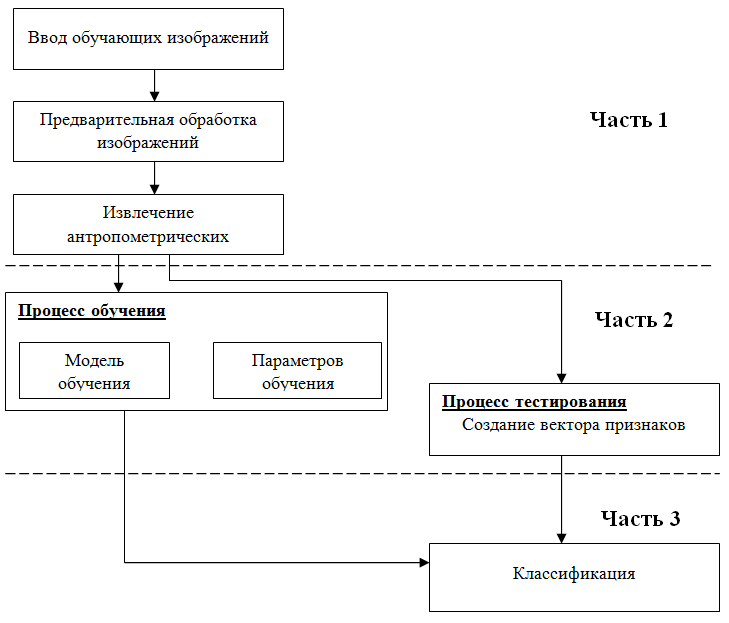
\includegraphics [scale=0.8] {images/h7.png}
\begin{center}
%\captionsetup{justification=justified, labelsep=period}
\caption{Блок-схема антропометрической системы} \label{img7}
\end{center}
\end{figure}
Система предназначена для использования в различных областях, таких как интернет-магазины для помощи пользователям в выборе размера одежды и фитнес-приложения.
%-------------------------
\section{Алгоритм извлечения антропометрических признаков из видео}

Процесс извлечения антропометрических признаков включает следующие этапы:

\begin{itemize}
	\item Предварительная обработка и нормализация изображения: на этом этапе необходимо выполнить фильтрацию шума и сглаживание изображения, применить морфологические операторы для улучшения качества контура объекта, для увеличения диапазона яркости изображений провести эквализацию их гистограмм (представлено в разделе \ref{part2.2.1});
	\item Использование алгоритма вычитания фона для обнаружения объектов: На этом шаге применяется два различных алгоритма: вычитание фона и на основе метода порогового значения. Применение для изображений и видео, полученных с камеры (представлено в разделе в \ref{part2.2.2});
	\item Использование алгоритма сегментации изображений и поиска ближайших точек границы чтобы найти местонахождение и контуры частей человеческого тела. На этом шаге применяется алгоритм разреза на графах для сегментации изображений и поиска частей человеческого тела, алгоритм обнаружения контура, итеративный алгоритм ближайших точек (Iterative Closest Point-$ICP$) для определения и корректировки точек признаков, которые ближе всего к их фактическим границам;
	\item Сравнительный анализ извлеченых признаков с реальными объектами для проверки точности методов и алгоритмов компьютерного зрения: на этом этапе будут сравниваться геометрические особенности частей человеческого тела с их настоящими частями, размеры которых были извлечены из реального тела, чтобы настроить соответствующие параметры.
\end{itemize}

В данной работе предложен метод извлечения антропометрических признаков из изображений и видео на основе алгоритмов компьютерного зрения предложенного подхода к задаче автоматического извлечения антропометрических признаков в режиме реального времени.


\input{part1/part1_2_1}
%-------------------------
\input{part1/part1_2_2}
%-------------------------
\input{part1/part1_2_3}
%-------------------------
\input{part1/part1_2_4}
%-------------------------
\input{part1/part1_2_5}
%-------------------------
%-------------------------
\section{Оценивание точности метода извлечения антропометрических признаков}
В этой части представлен результат извлечения антропометрических признаков на основе алгоритма компьютерного зрения из $50$ изображений. Извлечение ключевых точек (меток - опорных точек) состоит из $2$ главных этапов:

\begin{itemize}
	\item \textbf{Шаг 1:} Предварительная обработка изображения, преобразование исходного цветного изображения в изображение в оттенках серого, фильтрация шумов, разряжение пикселей, эквализация гистограммы для получения лучшего качества изображения;
	\item \textbf{Шаг 2: } Извлечение точек признаков с использованием алгоритма вычитания фона, обнаружения человеческого лица, сегментации изображения, поиска опорных точек для вычисления антророметрических признаков.
\end{itemize}

Для оценки эффективности процесса извлечения признаков применяются средняя абсолютная ошибка - $MAPE$:
\begin{equation}\label{eq26}
M=\frac{1}{n}\sum^n_{i=1}\left|\frac{A_t-F_t}{A_t}\right|,
\end{equation}
Где:

\begin{itemize}
	\item $A_t$: Результат измерений, рассчитанных вручную;
	\item $F_t$: Результат извлечения антропометрических признаков.
\end{itemize}
Эксперимент был использован для проверки погрешности размеров человеческих частей на основе извлечения количества признаков. На основании результатов для калибровки точности алгоритма.

\textbf{Случай 1}: Результат извлечения 24 опорных точек на контуре человеческого тела. Иллюстрация расположения опорных точек (рис. \ref{img15}): 
\begin{figure}[ht!]
\centering
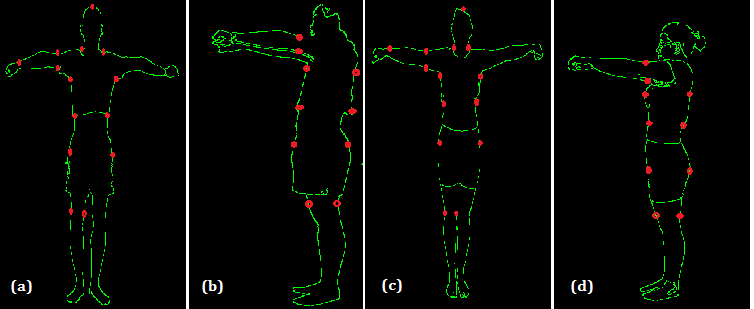
\includegraphics [scale=0.8] {images/h15.png}
\begin{center}
%\captionsetup{justification=justified, labelsep=period}
\caption{Результат расположения 24 опорных точек \cite{long1,long2}.} \label{img15}
\end{center}
\end{figure}

\begin{table}[b!]%
\begin{center}
\caption{Результат извлечения антропометрических признаков и погрешности системы компьютерного зрения \cite{long1,long2}.}\label{tab1}
  \begin{tabular}{|c|c|c|c|c|c|c|}
    \hline
    \multirow{2}{*}{Антропометрические} & {Ручной} & \multicolumn{3}{c}{Результаты системы} & {$\sum^n_{i=1}\left|\frac{A_t-F_t}{A_t}\right|$} &{$M$} \\
      признаки& метод &1 &2 &3& & \\
    \hline
Груди &95	&93.65	&94.11	&93.32	&0.04126	&0.01375\\
\hline
Талия               &79	&76.06	&78.80	&80.15	&0.05430	&0.01810\\
\hline
Бедра               &96.5	&93.07	&95.19	&95.78	&0.05658	&0.01886\\
\hline
Длина рук           &53	  &52.45	&54.32	&54.72	&0.06774	&0.02258\\
\hline
Обхват бицепса      &28	 &25.68	  &27.09	&27.60	&0.12964	&0.04321\\
\hline
Обхват шеи          &37	 &35.71	  &36.67	&36.79	&0.04946	&0.01649\\
\hline
Длина спины         &40	 &38.50	  &40.11	&40.01	&0.04050	&0.01350\\
\hline
Длина плеча       &36	 &35.86	  &36.19	&35.50	&0.02306	&0.00769\\
\hline
Ширина плеча         &14	 &13.91	  &13.56	&14.74	&0.09071	&0.03024\\
\hline
Высота груди        &18	 &17.78	  &17.60	&17.86	&0.04222	&0.01407\\
\hline
  \end{tabular}
\end{center}
\end{table}%\vspace{10mm}

\textbf{Случай 2:} Применение метода калибровки для улучшения точности извлечения признаков (рис. \ref{img152}).
\begin{figure}[ht!]
\centering
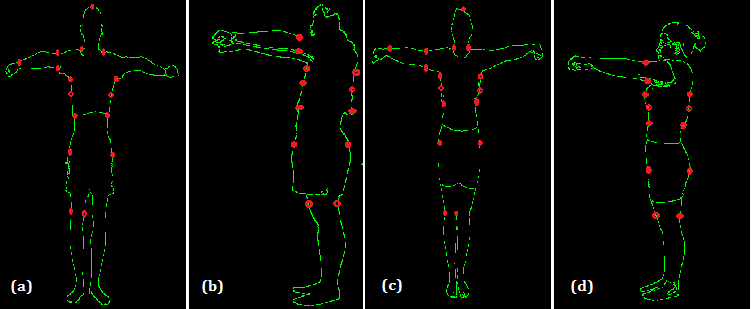
\includegraphics [scale=0.8] {images/h152.png}
\begin{center}
%\captionsetup{justification=justified, labelsep=period}
\caption{Результат расположения 28 опорных точек  \cite{long1,long2}.} \label{img152}
\end{center}
\end{figure}
\begin{table}[b!]%
\begin{center}
\caption{Результат извлечения антропометрических признаков и погрешности системы компьютерного зрения после применения калибровки извлеченных точек \cite{long1,long2}.}.\label{tab3}
  \begin{tabular}{|c|c|c|c|c|c|c|}
    \hline
    \multirow{2}{*}{Антропометрические} & {Ручной} & \multicolumn{3}{c}{Результаты системы} & {$\sum^n_{i=1}\left|\frac{A_t-F_t}{A_t}\right|$} &{$M$} \\
      признаки& метод  &1 &2 &3 & & \\
    \hline
Груди &95	&95.03	&95.00	&95.02	&0.00053	&0.00018 \\
\hline 
Талия             &79	&78.46	&79.05	&78.89	&0.00557	&0.00186\\

\hline
Бедра               &96.5	&97.29	&96.11	&96.4	&0.00010	&0.00003\\

\hline
Длина рук           &53	&52.93		&52.1	&52.93	&0.03531	&0.01177\\

\hline
Обхват бицепса      &28	&28.24	&28.03	&28.07	&0.01071	&0.00357\\

\hline
Обхват шеи         &37	&38.35	&38.13	&38.05	&0.09672	&0.03224\\

\hline
Длина спины         &40	&38.35	&39.96	&39.81	&0.04325	&0.01442\\

\hline
Длина плеча       &36	&36.01	&36.17	&36.1	&0.00971	&0.00324\\

\hline
Ширина плеча        &14	&13.97	&14.02	&14.02	&0.00071	&0.00024\\

\hline
Высота груди       &18	&18.05	&18.11	&18.01	&0.01500	&0.00500\\

\hline
  \end{tabular}
\end{center}
\end{table}%\vspace{10mm}

\begin{figure}[ht!]
\centering
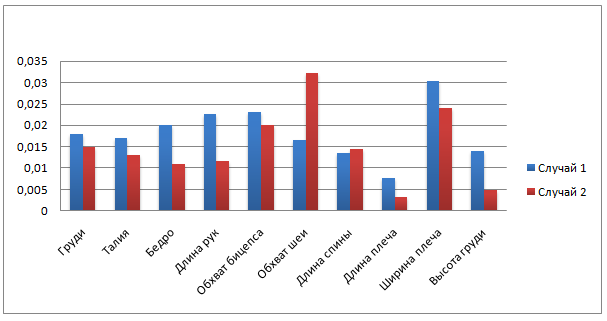
\includegraphics [scale=0.7] {images/h16.png}
\begin{center}
%\captionsetup{justification=justified, labelsep=period}
\caption{Погрешность в обоих случаях в извлечении антропометрических признаков.} \label{img16}
\end{center}
\end{figure}

\begin{figure}[ht!]
\centering
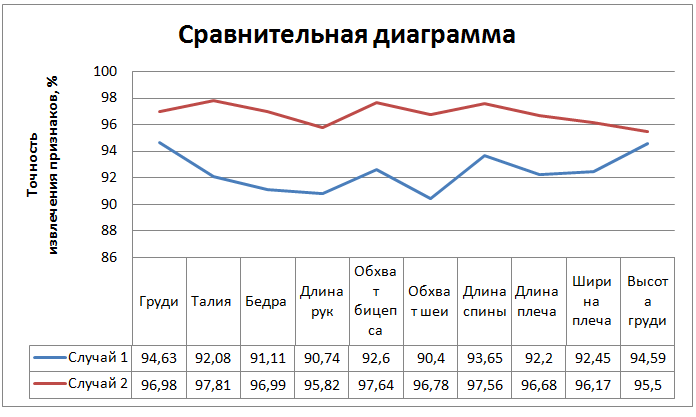
\includegraphics [scale=0.7] {images/h18.png}
\begin{center}
%\captionsetup{justification=justified, labelsep=period}
\caption{Процент правильной классификации (\%)  в обоих случаях в извлечении антропометрических признаков.} \label{img18}
\end{center}
\end{figure}

Для вычичления технической погрешности измерений при извлечении антропометрических признаков используется метод $TEM$(technical error of measurement)\cite{Stanley1999}. В данной работе выполняется извлечение антропометрических признаков 100 раз для одного человека.

С помощью метода $TEM$:

	\begin{equation}\label{eq50}
TEM=\sqrt{\left(\left(\sum_1^N\left(\left(\sum_1^K M^2\right)-\left(\left(\sum_1^K M\right)^2\right)\right)\right)/N\left(K-1\right)\right)}
\end{equation}
Где

\begin{itemize}
	\item $N$ - количество объектов;
	\item $K$ - количество выполнения;
	\item $M$ - измерение.
\end{itemize}

Получена гистограмма технической погрешности измерений (рис. \ref{img45}).

\begin{figure}[ht!]
\centering
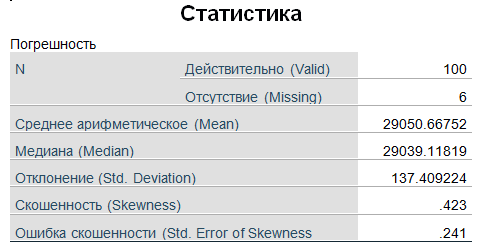
\includegraphics [scale=1] {images/h45.png}
\begin{center}
%\captionsetup{justification=justified, labelsep=period}
\caption{Результат анализа погрешности.} \label{img45}
\end{center}
\end{figure}

В (рис. \ref{img45}) показано, что среднее арифметичесное $mean = 29050.66752$, медиана $median = 29039.11819$ и скошенность $skewness= 0.423$. В этом распределении среднее арифметичесное и медиана приблизительны, скошенность $\in \left[-1;1\right]$. Поэтому это нормальное распределение (распределение Гаусса) (рис. \ref{img44}).

\begin{figure}[ht!]
\centering
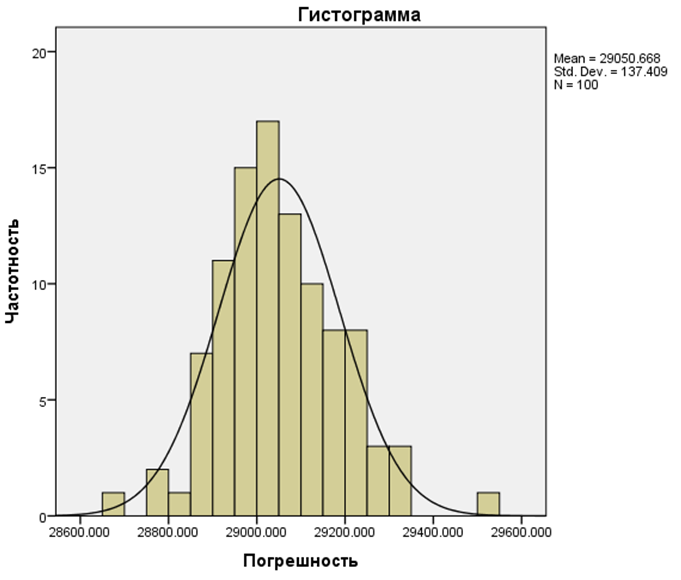
\includegraphics [scale=1] {images/h44.png}
\begin{center}
%\captionsetup{justification=justified, labelsep=period}
\caption{Гистограмма технической погрешности измерений.} \label{img44}
\end{center}
\end{figure}



  
%-------------------------
\section{Приложение алгоритма случайного леса для классификации антропометрических данных}
\subsection{Предложенная модель} В работе используется модель Wrapper \cite{Vladimir2000} с целевой функцией для оценки алгоритма случайного леса, показанная на рисунке (рис. \ref{img19}).
\begin{figure}[ht!]
\centering
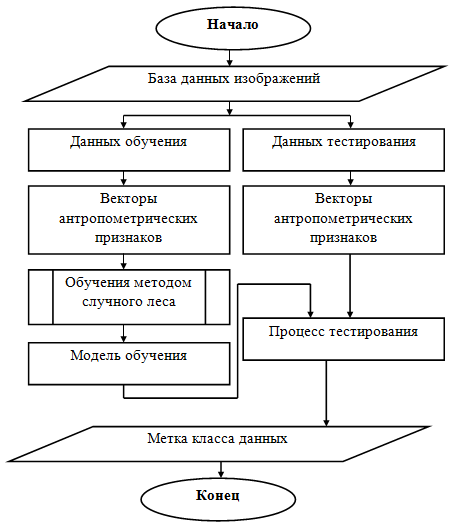
\includegraphics [scale=1] {images/h19.png}
\begin{center}
%\captionsetup{justification=justified, labelsep=period}
\caption{Предложенная модель} \label{img19}
\end{center}
\end{figure}
Архитектура системы состоит из двух основных частей. Часть $1$ используется, чтобы найти набор лучших атрибутов. Cистема генерирует наборы атрибутов, а затем использует алгоритм машинного обучения Random Forest для оценки таких наборов. Этот процесс повторяется до удовлетворения условий, чтобы остановить систему и получить набор оптимальных признаков. Часть $2$ используется, чтобы проверить подходит ли данная модель.
\subsection{Предложенный алгоритм}
В данной работе предлагается алгоритм случайного леса для классификации измерений для построения 3D модели на основе оценки и поиска набора антропометрических признаков из исходного набора признаков. Шаги выполнения алгоритма обозначается следующим образом:

\begin{itemize}
	\item \textbf{Шаг 1:} Создание $m$ наборов признаков из $n$ наборов первоначальных признаков. Каждый набор содержит $2 \frac{n}{m} $признаки. В том числе:
	
	\begin{itemize}
		\item  $\frac{n}{m}$ признаки равны;
		\item  $\frac{n}{m}$ случайные признаки.

	\end{itemize}
	
	\item \textbf{Шаг 2:} Использование Random Forest для того, чтобы вычислять оценку наборов признаков $\Rightarrow$ получение набора значений $f\left(i\right), i= \left(1,..., m\right)$;
	\item \textbf{Шаг 3:}взвешивание каждого признака $i$ рассчитывается по формуле:
	$w_j= \sum^m_{i=1}kf_i$;
	
	\begin{itemize}
		\item $k_{ij} = 0$, если признак $i$ не выбран в наборе признака $j$;
    \item $k_{ij}= 1$, если признак выбран в наборе признака $j$.
	\end{itemize}
	
	\item \textbf{Шаг 4:} Разработка нового признака включает в себя $р\%$ лучших признаков;
	\item \textbf{Шаг 5:} Повторение шага $1$ для удовлетворения одного из двух условий:
	
	\begin{itemize}
		\item Количество признаков < порога разрешено;
		\item Количество циклов определено.
	\end{itemize}
	
\end{itemize}

Изложенное выше направление рекомендуется для того, чтобы найти набор оптимальных маленьких признаков, таким образом, цель состоит в том, чтобы ограничить количество выходных признаков. Эти первоначальные признаки разделены для обеспечения всех выбранных признаков. Затем в сочетании с делением случайных признаков, создаются новые маленькие наборы признаков. Дальше алгоритм машинного обучения случайного леса используется для вычисления актуальности набора признаков. На основе значения расчетного уровня вычисления мы находим набор признаков, которые имеют меньшее количество свойств при сохранении целей работы.
\subsection{Формирование опорных точек с признаками объектной принадлежности}
В этом разделе представлен подход к реконструкции 3D-модели человека на основе антропометрических признаков, которые были извлечены и классифицированы из 2D-изображений. Мы используем набор данных  антропометрических признаков для построения 3D-модели точной и эффективной в соответствии с формой и фактическим размером объекта.

Процесс построения 3D-модели включает следующие шаги:

\begin{itemize}
	\item Шаг 1: Описание текстурных характеристик человеческого тела (кожа, волосы, лицо), а также текстуры одежды;
   \item Шаг 2: Разработка частей человеческого тела (голова, туловище, руки, ноги) с использованием ранее полученных антропометрических признаков;
\item Шаг 3: Комбинация текстуры и частей человеческого тела в блок;
\item Шаг 4: Экспорт антропометрических моделей человеческого тела в два файла: первый файл (*.mtl) описывает текстуры модели, второй файл (*.obj) содержает информацию каждой модели.
\end{itemize}

Алгоритм для соответствия 3D-модели с антропометрическими признаками:
\begin{figure}[ht!]
\centering
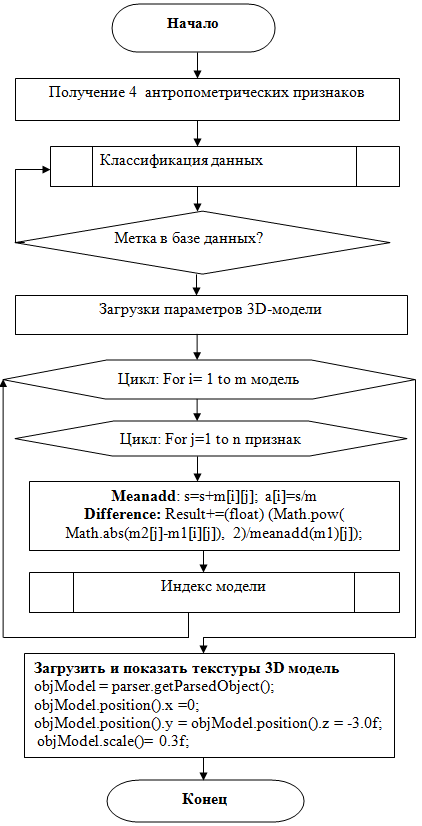
\includegraphics [scale=1] {images/h21.png}
\begin{center}
%\captionsetup{justification=justified, labelsep=period}
\caption{Алгоритм сопоставления 3D-формы с данными маркировки} \label{img21}
\end{center}
\end{figure}

\textbf{Результаты и анализ экспериментов на наборах антропометрических данных}

\textbf{Часть 1:} Обучение базового алгоритма случайного леса на наборах антропометрических данных выполнены $5$ раз с использоване библиотеки Weka \cite{Weka}. Каждый раз запуска будет диагонально выполнять проверки с количеством деревьев соответственно $100$, $200$, $300$, $400$, $500$ мы получим результат( в таблице \ref{tab5}):

\begin{table}[b!]%
\begin{center}
\caption{Результаты классификации на основе алгоритма случайного леса \cite{long1,long2}}\label{tab5}
  \begin{tabular}{|c|c|c|c|c|}
    \hline
 Количество  & Среднее   &   Стандартное   & Минимальное   & Максимальное \\
деревьев     & значение  &    отклонение   & значение      &значение      \\
\hline
100 &	0.03480	&0.025&	0.0139&	0.0606\\
\hline
200 &	0.02761	&0.0200	&0.0152	&0.0352\\
\hline
300	&0.02178	&0.0125	&0.0121	&0.0336\\
\hline
400	&0.01830	&0.0150	&0.0076	&0.0270\\
\hline
500	&0.01661	&0.0115	&0.0102	&0.0254\\
\hline

  \end{tabular}
\end{center}
\end{table}%\vspace{10mm}

\textbf{Часть 2:} Выбор набора оптимальных данных из наборов антропометрических данных мужчин первоначально предложенными методами выше. С начальным набором признаков, мы делим на m подразделение наборов признаков с использованием функции выборки <<$sample\left(, ,replace=True\right)$>> так что каждый набор содержит $\frac{n}{m}$ распределеные равномерные признаки и $\frac{n}{m}$ случайные признаки. Где $n$ - общее число признаков, $m$ - параметр распределения (в эксперименте выбрать $m=4$). В частности, файл результата <<ImportantFeature>> показывает новый набор, который включает в себя $4$ признака, расположенных соответственно в $12$ первоначальных признаках: $5,6,7,10$. С новым набором признаков, мы ещё раз выполняем часть $1$ представленную выше и получим результаты случайного леса при запуске пяти новых наборов признаков, показанных в таблице (\ref{tab6}).

\begin{table}[b!]%
\begin{center}
\caption{Результаты классификации на основе алгоритма случайного леса \cite{long1,long2}}\label{tab6}
  \begin{tabular}{|c|c|c|c|c|}
    \hline
  Количество  & Среднее   &   Стандартное   & Минимальное   & Максимальное \\
деревьев     & значение  &    отклонение   & значение      &значение      \\
\hline
100	&0.0116	&0.00833	&0.00463	&0.0202\\
\hline
200	&0.0092	&0.00667	&0.00516	&0.0117 \\
\hline
300	&0.02178	&0.00416	&0.0040	&0.0221\\
\hline
400	&0.00726	&0.0050	&0.0071	&0.009\\
\hline
500	&0.00553	&0.00383	&0.00513	&0.0085\\
\hline
  \end{tabular}
\end{center}
\end{table}%\vspace{10mm}

\subsubsection{Применение результатов классификации для построения 3D-моделей}
В работе \cite{grudinin2009} посвящена анализу антропометрических характеристик человеческого тела с целью определения границ изменения параметров и их взаимосвязи в рамках задачи параметрического моделирования компьютерных манекенов. В \cite{grudinin2014} предложен моделирование нестандартных параметризованных манекенов в рамках параметрического представления сложных геометрических объектов, удовлетворяющих заданным антропометрическим данным. Результаты исследований сосредоточены на построении частей человеческого тела: грудь и талию. Срок реализации 1-5 минут. В нашей работе используется результат классификации антропометрических данных, которые важные для построения антропологических моделей. При таком подходе, время работы программы быстрее и обеспечивает полную модель человеческого тела.

На основе выходных результатов процесса классификации - метка класса присваивается после процесса проверки. Основываясь на значении метки класса каждой записи, имеющееся $3D$-модель соответствует и подходит с параметрами каждой записи. $3D$-модели были построены при поддержке библиотек Min3D \cite{Min3D} и MakeHuman \cite{Make}. База данных включает в себя $100$ построенных моделей, в соответствии с размерами тела $XS$, $S$, $M$, $L$, $XL$. Каждый размер тела имеет $20$ моделей, построенных на основе каждого различного параметра тела.

На основе результата тестов, у нас имеется $5$ записей помеченых метками: $1$, $2$, $3$, $4$, $5$. Значит в очереди, записи имеют $3D$-модели соответствующие размерам $XS$, $S$, $M$, $L$, $XL$. Выбор наиболее подходящей модели для каждой записи будет основываться на $4$ признаках, которые выбраны из предлагаемого алгоритма: обхват груди $\left(B\right)$, обхват талии $\left(W\right)$, обхват бедер $\left(C\right)$, рост $\left(H\right)$. Мы создаем формулу для расчета следующим образом:
\begin{equation}\label{eq26}
Model = Min\left\{\sum^N_{i=1}\left(B-B_i\right)^2+\left(C-C_i\right)^2+\left(W-W_i\right)^2+\left(H-H_i\right)^2\right\}.
\end{equation}
Применение результатов алгоритма классификации случайного леса повышает точность результатов и уменьшает время вычисления в программе. График сравнения среднего времени при запуске случайного леса $5$ раз на новые наборы и начальные наборы антропометрических данных с количеством деревьев соответственно $100$, $200$,$300$, $400$, $500$ (рис. \ref{img20}).
\begin{figure}[ht!]
\centering
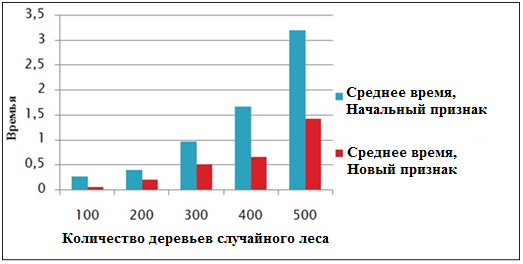
\includegraphics [scale=1] {images/h20.png}
\begin{center}
%\captionsetup{justification=justified, labelsep=period}
\caption{Время работы классификации для каждого набора данных.} \label{img20}
\end{center}
\end{figure}
%-------------------------
\section{Основные результаты и выводы по главе 2}

\begin{enumerate}
	\item Предложен метод извлечения антропометрических признаков на изображениях и видео на основе алгоритмов компьютерного зрения. Проведено улучшение качества изображения с помощью технической обработки изображений, обнаружение объектов с помощью алгоритма вычитания фона, сегментации изображения с помощью алгоритма разреза на графах, извлечения ключевых точек методом $ICP$;
 \item Предложен метод поправочного множителя с использованием комбинированного алгоритма $ICP$ для повышения точности извлечения антропометрических признаков на изображениях и видео.
\item Предложен метод классификации антропометрических данных с помощью алгоритма случайных лесов - Random Forest для классификации размеров и $3D$ моделей человеческого тела.
\item Предложена модель классификации Wrapper и алгоритм извлечения важных признаков для повышения точности и скорости алгоритма случайного леса.
\item Разработан алгоритм и схема его применения для извлечения и классификации антропометрических данных с помощью алгоритмов компьютерного зрения.
\item На основе численных экспериментов проведен сравнительный анализ применимости и сравнение возможности применения алгоритмов компьютерного зрения в антропометрии - обнаружение объектов с помощью алгоритма вычитания фона, сегментации изображения с помощью алгоритма разреза графов, извлечения ключевых точек методом $ICP$, классификации антропометрических данных с помощью алгоритма случайных лесов для решения проблемы в  антропометрии на статических изображениях в присутствии шума. 
\item Экспериментальные результаты представлены в таблицах (\ref{tab1}), (\ref{tab3}), (\ref{tab5}), (\ref{tab6}) показывают, что алгоритмы работают с высокой скоростью и точностью при извлечении и классификации антропометрических данных на изображениях и на видеопоследовательностях в присутствии шума и в реальном режиме времени. 

\end{enumerate}

%-------------------------


%%\chapter{Нелинейные интегральные уравнения Вольтерра I рода с кусочно-непрерывными ядрами} \label{chapt2}
%\chapter{Интегральные модели Вольтерра на основе нелинейных уравнений} \label{chapt2}
%\chapter{Интегральные модели развивающихся динамических систем на основе нелинейных уравнений Вольтерра I рода с разрывными ядрами} \label{chapt2}
%\section{Интегральные модели развивающихся динамических систем на основе нелинейных уравнений Вольтерра I рода с разрывными ядрами} \label{chapt2}


%\section{Постановка задачи} \label{sect2_1}
\chapter{Системный анализ и проектирование построения систем компьютерного зрения в антропометрии. Тестирование и разработка алгоритмов компьютерного зрения на изображении и видео}
В данной главе приводятся информация о анализе, проектировании и построении антропометрического пакета прикладных программ с помощью  объектно-ориентированного языка UML. При анализе результатов испытаний применяются алгоритмы компьютерного зрения в условиях шума, и в режиме реального времени.


\section{Анализ и проектирование системы компьютерного зрения в антропометрии}
Жизненный цикл программы в целом не может быть разделен на периоды. Он описывает процесс создания, тестирования и поддержания работы системы \ref{img33}.

\begin{figure}[ht!]
\centering
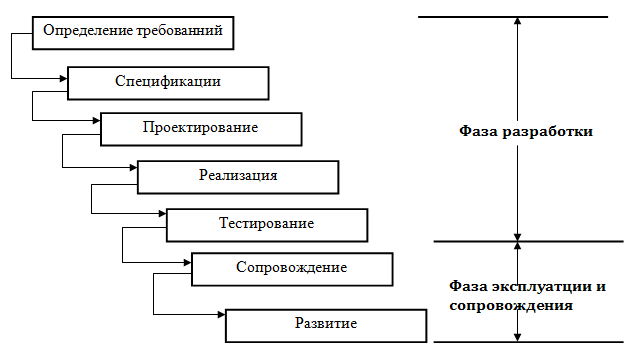
\includegraphics [scale=1] {images/h33.png}
\begin{center}
%\captionsetup{justification=justified, labelsep=period}
\caption{Общепринятая модель жизненного цикла программного обеспечения.} \label{img33}
\end{center}
\end{figure}

В данной работе подробно описан этап проектирования системы. Для этого было создано хранилище документов проекта, включающее в себя: теории и модели, методы и инструменты, используемые для создания и развития системы. Анализ и проектирование системы основаны на двух факторах: 

\begin{itemize}
	\item Понимание целей, структуры и процессов работы системы;
  \item Применение передовых методов и соответствующих алгоритмов для повышения эффективности работы и точности системы.

\end{itemize}
Особенностью анализа и объектно-ориентированного проектирования является система, включающая в себя совокупность объектов, взаимодействующих друг с другом для выполнения задачи с  достижением более высоких результатов. Для достижения этой цели мы должны использовать системные модели объектов со следующими основными характеристиками:

\begin{itemize}
	\item С высокой абстракцией;
  \item По состоянию упаковочной информации;
  \item Модуль;
  \item Наследование.

\end{itemize}
Сегодня UML является инструментом, обладающим  всеми характеристиками и условиями,о которых говорилось выше, для построения модели объекта. UML - графический язык для документирования, конструирования, описания параметров и визуализации абсолютно различных систем (программ в частности).
Графики моделирования объектов представлены в диссертации, в том числе:

\begin{itemize}
	\item \textbf{Диаграмма прецедентов} (Use Case diagram) - диаграмма, отражающая отношения между актёрами и прецедентами, являющаяся составной частью модели прецедентов, позволяющей описать систему на концептуальном уровне;
\item \textbf{Диаграмма классов} (Static Structure diagram) - диаграмма, демонстрирующая классы системы, их атрибуты, методы и взаимосвязи между ними. Входит в UML;
\item \textbf{Диаграмма последовательности} (sequence diagram): диаграмма, на которой для некоторого набора объектов на единой временной оси показан жизненный цикл (создание-деятельность-уничтожение) и взаимодействие (отправка запросов и получение ответов). Используется в языке UML.

\end{itemize}

Объектная модель описывает структуру объектов, их операции, атрибуты  и взаимосвязи с другими объектами. Объектная модель показывает понятия и реальные объекты, которые важны для разрабатываемой системы. Цель разработки объектной модели - выделение и описание объектов, составляющих проектируемую систему и выявление различных зависимостей между объектами.

Система компьютерного зрения в антропометрии включает в себя следующие основные вопросы:

\begin{itemize}
	\item Сбор и обработка данных с камеры;
	\item Извлечение антропометрических признаков;
	\item Классификация антропометрических данных;
	\item Разработка приложений для текстильной промышленности (E-Tailor) и фитнеса (E-фитнес) на основе результатов системы компьютерного зрения в антропометрии.
\end{itemize}

\begin{figure}[ht!]
\centering
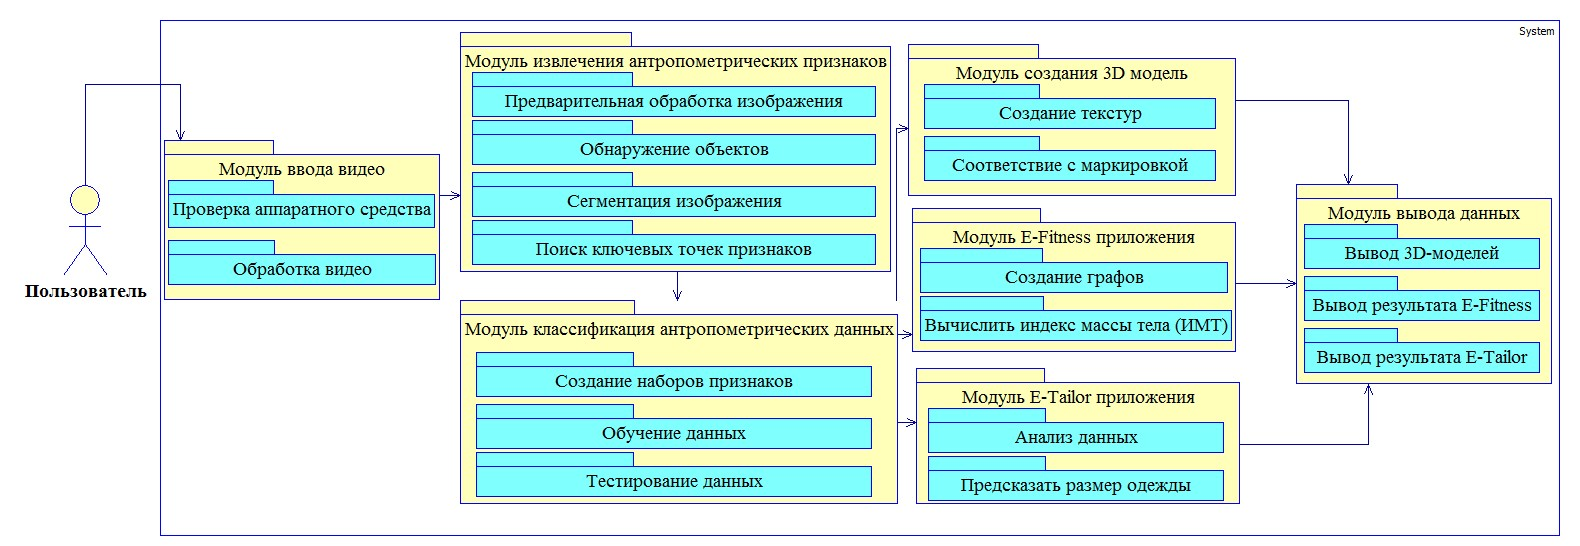
\includegraphics [scale=0.4] {images/h35.png}
\begin{center}
\caption{Структура ПО} \label{img35}
\end{center}
\end{figure}

\subsection{Анализ и проектирование системы компьютерного зрения в антропометрии для текстильной промышленности}

\textbf{Цель}: Описание работы программы автоматического измерения размеров человеческого тела, 3D моделирование тела мужчины / женщины, выбор размеров одежды на основе антропометрических признаков.

Система состоит из одного главного фактора: пользователи. Система имеет основные функции:

\begin{itemize}
	\item Сбор данных с камеры;
	\item Заполнение информации о росте, весе;
	\item 3D-моделирование человеческого тела;
	\item Классификация и предсказание размеров одежды;
	\item Контакты с командой разработчиков.

\end{itemize}
\begin{figure}[ht!]
\centering
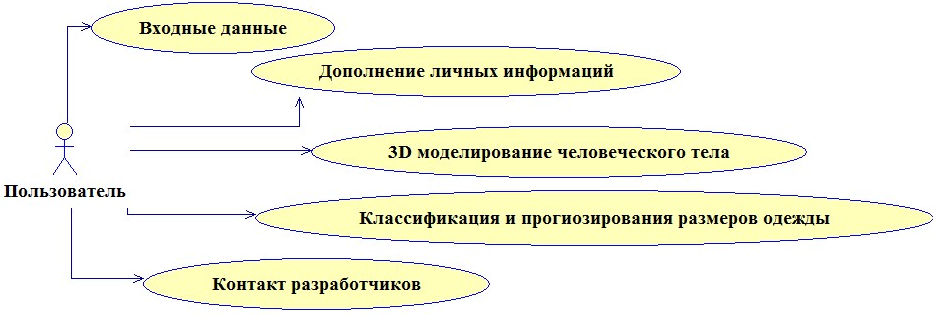
\includegraphics [scale=0.5] {images/h22.png}
\begin{center}
%\captionsetup{justification=justified, labelsep=period}
\caption{Диаграмма прецедентов - использование системы компьютерного зрения приложения E-Tailor.} \label{img22}
\end{center}
\end{figure}
\begin{figure}[ht!]
\centering
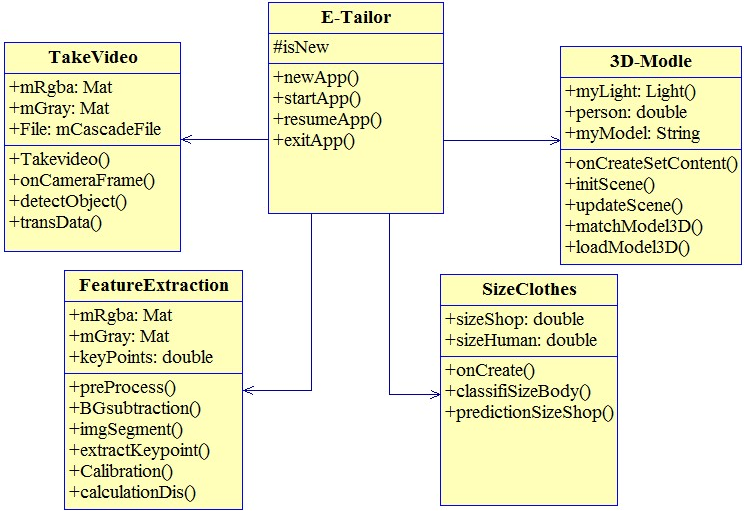
\includegraphics [scale=0.5] {images/h23.png}
\begin{center}
%\captionsetup{justification=justified, labelsep=period}
\caption{Диаграмма классов - система компьютерного зрения в антропометрии приложения E-Tailor.} \label{img23}
\end{center}
\end{figure}
\begin{figure}[ht!]
\centering
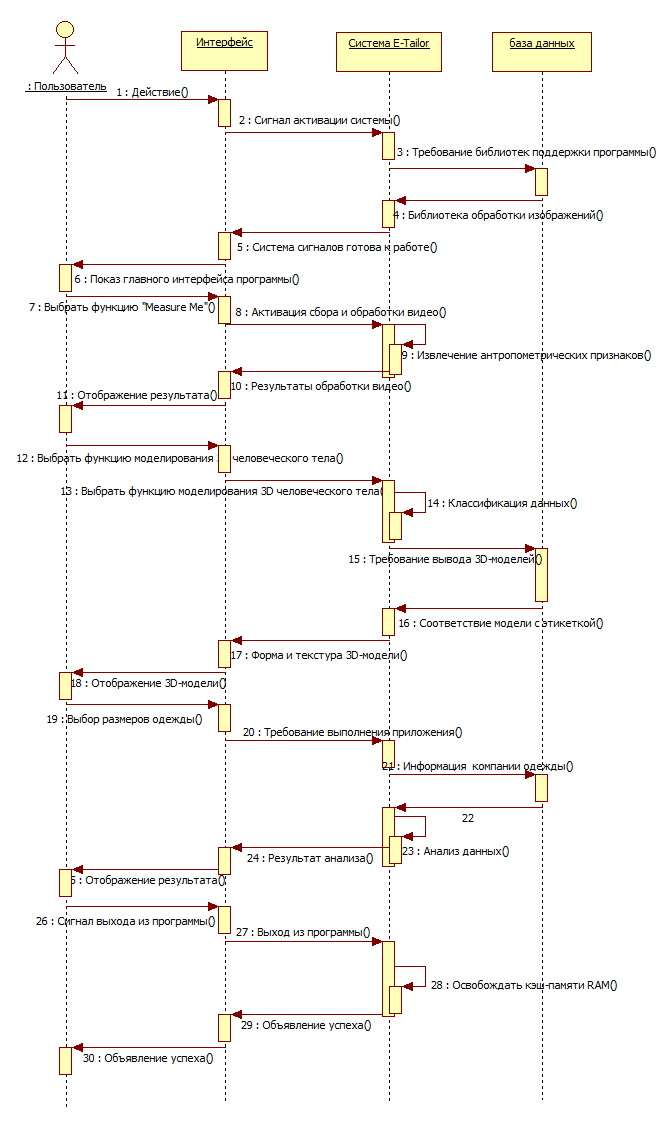
\includegraphics [scale=0.8] {images/h28.png}
\begin{center}
%\captionsetup{justification=justified, labelsep=period}
\caption{Диаграмма последовательности - система компьютерного зрения в антропометрии приложения E- Tailor.} \label{img28}
\end{center}
\end{figure}

\subsection{Анализ и проектирование системы компьютерного зрения в антропометрии для фитнеса}
\textbf{Цель}: Описание работы программы автоматического измерения размеров человеческого тела, 3D моделирование тела мужчины / женщины, автоматизация измерения индекса массы тела (ИМТ), анализ антропометрических признаков по стандартам фитнеса.

Система состоит из одного главного фактора: пользователи. Система имеет основные функции:

\begin{itemize}
	\item Сбор данных с камеры;
	\item Заполнение информации о росте, весе;
	\item 3D-моделирование человеческого тела;
	\item Анализ антропометрических признаков по стандартам фитнеса;
	\item Анализ ожирения в соответствии с индексом ИМТ;
	\item Тренажерные упражнения фитнеса в домашних условиях;
	\item Контакты с командой разработчиков.

\end{itemize}
\begin{figure}[ht!]
\centering
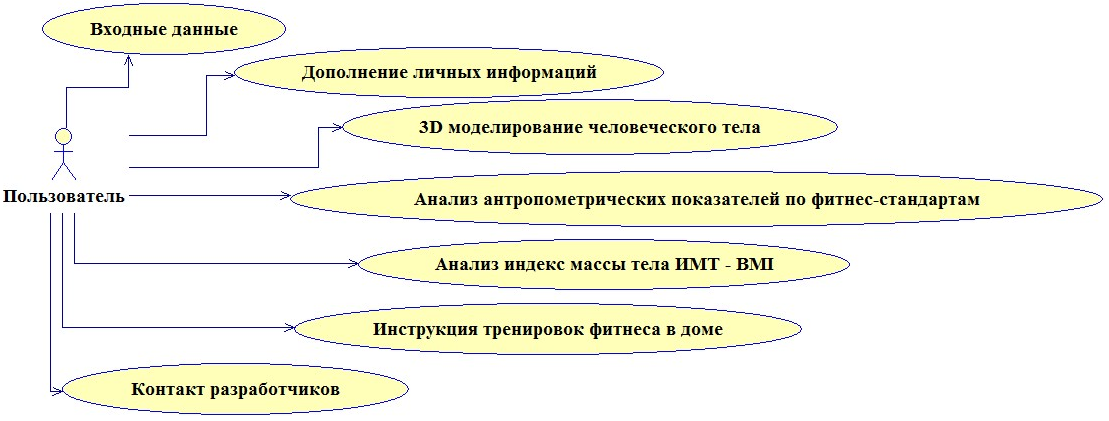
\includegraphics [scale=0.5] {images/h25.png}
\begin{center}
%\captionsetup{justification=justified, labelsep=period}
\caption{Диаграмма прецедентов - использование системы компьютерного зрения приложения E-Fitness.} \label{img25}
\end{center}
\end{figure}
\begin{figure}[ht!]
\centering
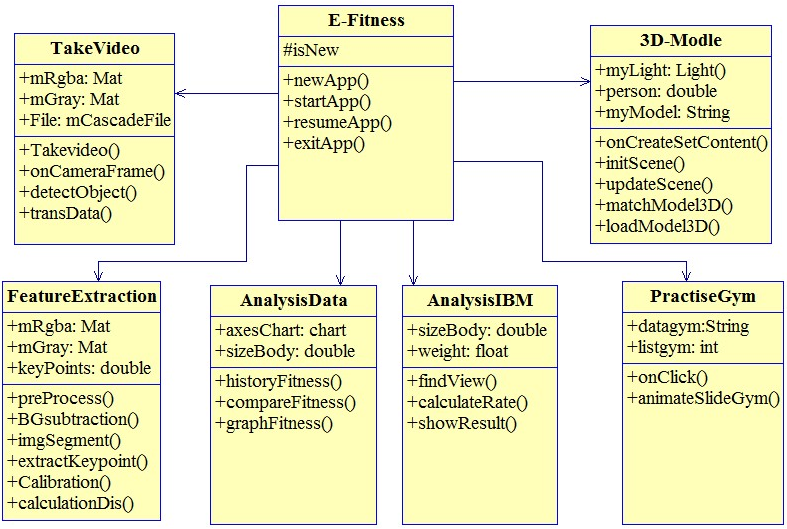
\includegraphics [scale=0.5] {images/h26.png}
\begin{center}
%\captionsetup{justification=justified, labelsep=period}
\caption{Диаграмма классов - система компьютерного зрения в антропометрии приложения E- Fitness.} \label{img26}
\end{center}
\end{figure}
\begin{figure}[ht!]
\centering
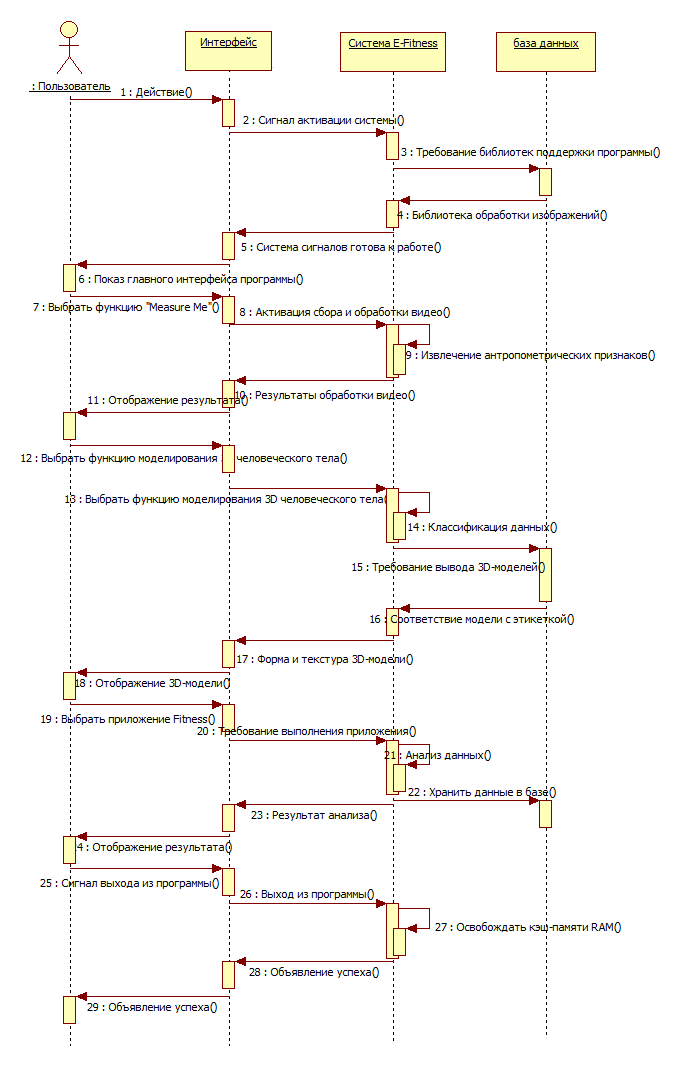
\includegraphics [scale=0.8] {images/h27.png}
\begin{center}
%\captionsetup{justification=justified, labelsep=period}
\caption{Диаграмма последовательности - система компьютерного зрения в антропометрии приложения E- Fitness.} \label{img27}
\end{center}
\end{figure}
%-------------------------
\section{Тестирование и разработка алгоритмов компьютерного зрения на изображении и видео}
\subsection{Эксперимент}
Цель эксперимента состояла в том, чтобы проверить эффективность работы алгоритмов, методов компьютерного зрения в антропометрии, проверить обоснованность конструкции системы, учитывая влияние внешних факторов на точность алгоритма.

Система компьютерного зрения в антропометрии состоит из 3 основных частей: извлечение антропометрических признаков, классификация антропометрических признаков и применения их на практике. 

Процесс извлечения  антропометрических признаков выполняется следующим образом. Во-первых, происходит обнаружение и распознавание объектов методами вычитания фона и обнаружения лица человека. Следующим шагом является сегментация и определение ключевых точек с помощью метода разреза на графах (Graph cuts) и итеративного алгоритма ближайших точек (Iterative Closest Point - ICP). Процесс классификации антропометрических признаков состоит из двух частей: обучение и тестирование. Важным шагом в этом процессе является  создание учебной модели для классификации новых данных с высокой точностью. 

В данной работе рассматривается построение приложения компьютерного зрения в антропометрии для двух областей: пошив одежды и фитнес-тестирование. В этом разделе рассматривается возможность создания 3D-моделей, классифиции размеров человеческого тела, способность анализировать антропометрические данные в соответствии со стандартом IBM, Fitness и т.д. Также, сравнивается наш метод и алгоритм построения системы компьютерного зрения антропометрии и другие алгоритмы, чтобы найти подходящий для успешной реализации.

\subsection{Тестирование разработанного ПО – извлечение и классификация антропометрических признаков на видео}
Эксперимент проводился на основе языка C ++ (Visual Studio 2010), Java, Matlab с использованием открытой библиотеки компьютерного зрения - OpenCV, библиотеки моделирования 3D для компьютеров и смартфонов - Min3D и библиотеки дизайн 3D моделей - Humanmaker. 

\textbf{Оборудование тестирования:}

\begin{itemize}
	\item Ноутбук с процессором Intel Core 2 Duo (2.3 ГГц), 3 Гб оперативной памяти, камера 1,3 мегапикселей, которая передает 30 кадров в секунду с разрешением  $320 * 240$ пикселей;
	\item Смартфон Самсунг с фронтальной камерой 5 мегапикселей.

\end{itemize}
Эксперимент проводился на основе данных, собранных с помощью личного устройства. На этапе сбора данных пользователь стоит перед фронтальной камерой телефона (расстояние такое, чтобы тело полностью было в кадре), выполняется серия движений, поворот на 90 градусов налево, направо и наоборот. Первоначально будут собираться данные с изображения. Приложение идентифицирует объект, который появляется в кадре и определяет, человек это или нет (на основе обнаружения лица). Затем программа автоматически собирает и выполняет вычитание фона изображения, сегментацию частей человеческого тела, определяет ключевые точки на теле. Происходит калибровка для расчета антропометрических признаков.

Для проверки правильности работы программы, эксперименты проводились несколько раз для одного и того же объекта, в разном времени и месте, в различных условиях шума и освещения, таких как, эксперименты \ref{img29}.

\begin{figure}[ht!]
\centering
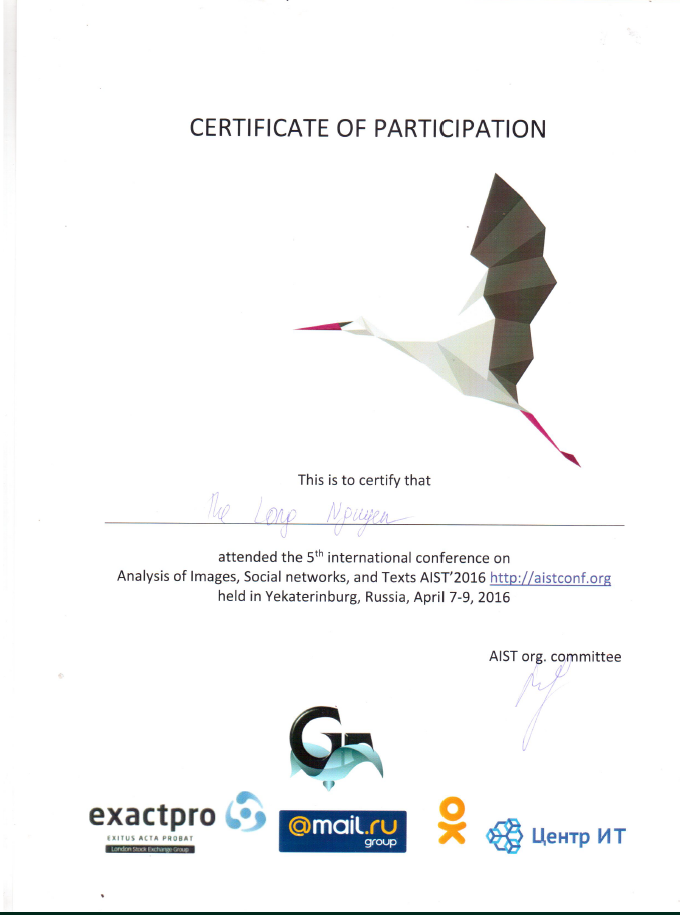
\includegraphics [scale=0.1] {images/h29.png}
\begin{center}
%\captionsetup{justification=justified, labelsep=period}
\caption{Пример данных эксперимента.} \label{img29}
\end{center}
\end{figure}

База данных для экспериментов на компьютере состоит из 6 видео. Эта база данных была создана, чтобы получить данные для тестирования и оценки эффективности работы методов и алгоритмов компьютерного зрения на видео. Создание этой базы необходимо, чтобы учитывать влияние различных факторов на производительность системы (\ref{img36}), (\ref{img37}).

\begin{figure}[ht!]
\centering
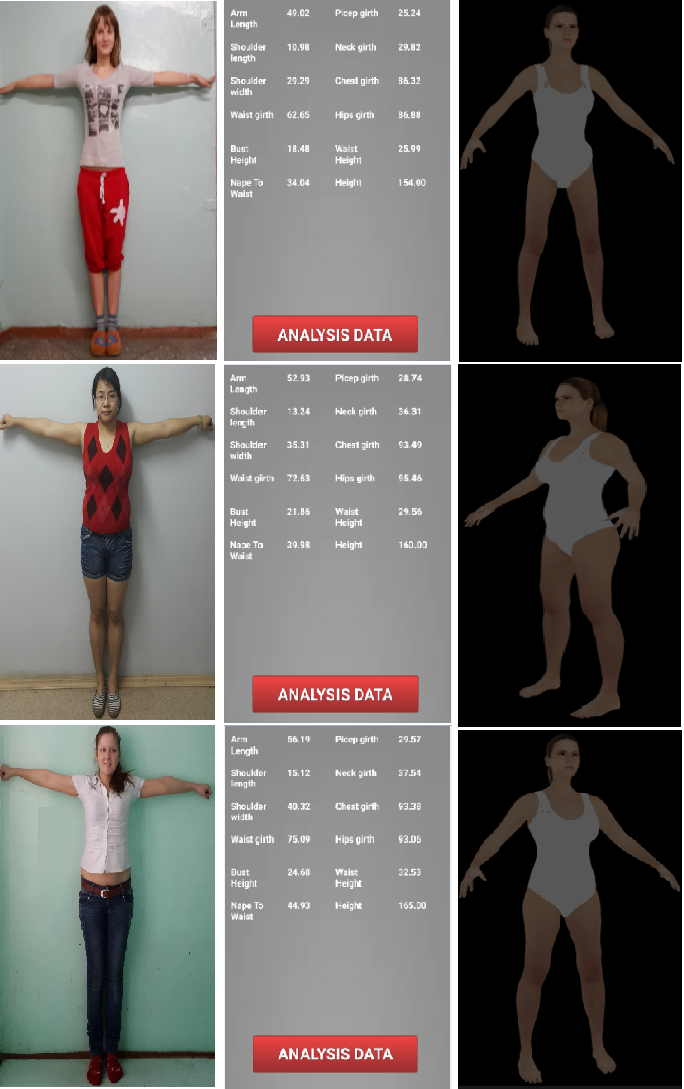
\includegraphics [scale=0.5] {images/h36.png}
\begin{center}
%\captionsetup{justification=justified, labelsep=period}
\caption{Результаты извлечения антропометрических признаков и 3D-моделей для женщин.} \label{img36}
\end{center}
\end{figure}
\begin{figure}[ht!]
\centering
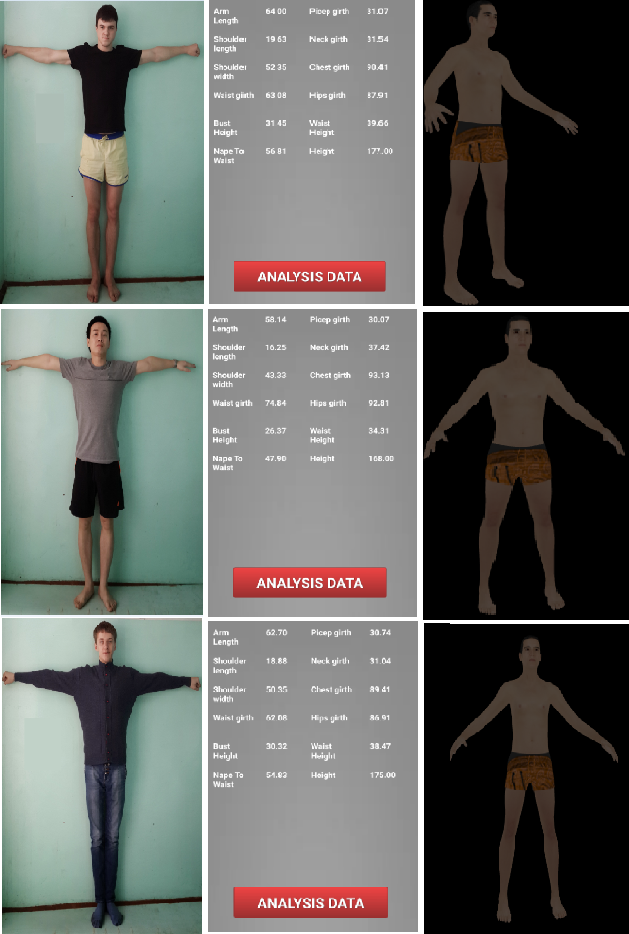
\includegraphics [scale=0.5] {images/h37.png}
\begin{center}
%\captionsetup{justification=justified, labelsep=period}
\caption{Результаты извлечения антропометрических признаков и 3D-моделей для мужчин.} \label{img37}
\end{center}
\end{figure}

В ходе эксперимента были использованы алгоритмы компьютерного зрения и извлечения антропометрических признаков. Для этого используются алгоритмы разреза на графах, а также итеративные алгоритмы ближайших точек двух видов: из 24 ключевых точек и 28 ключевых точек для сравнения результата алгоритма вычитания фона и метода выпуклой оболочки \ref{tab7} . В нашей работе \cite{long1} изложен метод измерения различных антропометрических признаков на основе анализа цифровых изображений. Для более эффективного измерения признаков предлагается использовать субпиксельную обработку и анализ выпуклой оболочки. В нашем подходе контур тела описывается выпуклостью дефектов треугольников. Тела представлены треугольниками. Такие треугольники имеют три координаты: выпуклый дефект старт, выпуклый дефект конец, и выпуклый дефект положения точек, соответственно помечены. Мы определили области интересов, которые содержат части тела. Таким образом, мы получили 5 выпуклых областей с соответствующими условиями.

\begin{table}[b!]%
\begin{center}
\caption{Результаты извлечения антропометрических признаков}\label{tab7}
\begin{tabular}{ |c|c|c|c| } 
\hline
  \multirow{3}{*}& Graph-cuts + ICP  & Graph-cuts + ICP  &Вычитание фона \\
								 & (28 ключевых - &(24 ключевых - & + выпуклая\\
	               & - точек)       & - точек)      & оболочка\\
\hline
\multirow{2}{*}{Груди} & \multicolumn{3}{|c|}{93}\\ 
                         & 92.85 & 90.75&85.0 \\ 
\hline
\multirow{2}{*}{Талия} & \multicolumn{3}{|c|}{75}\\ 
                         & 74.80 & 72.0 & 69.79 \\ 	
\hline
\multirow{2}{*}{Бедра} & \multicolumn{3}{|c|}{91}\\ 
                         & 91.3 & 89.65 & 88.65 \\ 
\hline
\multirow{2}{*}{Длина рук} & \multicolumn{3}{|c|}{50}\\ 
                         & 50.40 & 47.62 & 40.30 \\
\hline
\multirow{2}{*}{Обхват } & \multicolumn{3}{|c|}{29}\\ 
                бицепса  & 28.50 & 27.31 & 32.50\\
\hline
\multirow{2}{*}{Обхват } & \multicolumn{3}{|c|}{36}\\ 
                 шеи        & 36.21 & 35.70 & 38.95\\	
\hline
\multirow{2}{*}{Длина } & \multicolumn{3}{|c|}{40}\\ 
                 спины        & 40.10 & 38.75 & 56.50\\	
\hline
\multirow{2}{*}{Ширина } & \multicolumn{3}{|c|}{36}\\ 
                  плеча       & 36.25 & 34.30 & 31.90\\
\hline
\multirow{2}{*}{Длина } & \multicolumn{3}{|c|}{13}\\ 
                 плеча        & 13.10 & 12.83 & 15.56\\
\hline
\end{tabular}
\end{center}
\end{table}%\vspace{10mm}

В (рис. \ref{img24}) описан результат эксперимента проверки точности извлечения антропометрических признаков 3 методов (разреза на графах + ICP для 28 опорных точек, разреза на графах + ICP для 24 опорных точек, вычитание фона + выпуклая оболочка) с ручной метода для одного человека.

\begin{figure}[ht!]
\centering
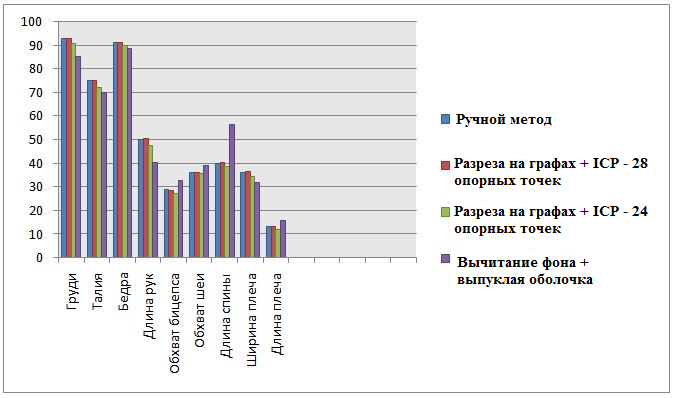
\includegraphics [scale=0.8] {images/h24.png}
\begin{center}
%\captionsetup{justification=justified, labelsep=period}
\caption{Сравнение результата эксперимента.} \label{img24} \label{img24}
\end{center}
\end{figure}

%-------------------------
\section{Основные результаты и выводы по главе 3}

\begin{enumerate}
	\item В этой главе описывается анализ проектирования систем компьютерного зрения в антропометрии для практических применений: пошив одежды и фитнес-тестирование с помощью аналитических методов объектно-ориентированного UML. Используются диаграммы прецедентов, диаграммы классов и диаграммы последовательности. Классы подробно анализируются, с указанием задач каждой компоненты в программе. Также обоснована целесообразность проектирования приложений компьютерного зрения;
	\item Описаны результаты тестирования алгоритмов компьютерного зрения, в том числе предварительной обработки изображений с помощью фильтра Гаусса, эквализация гистограммы, алгоритм вычитания фона изображения на основе фоновых модели, алгоритм сегментации изображений методом разреза на графах (graph cuts), итеративный алгоритм ближайших точек (Iterative Closest Point - ICP). Алгоритмы функционируют в режиме реального времени и в условиях наличия с шумов в видеопоследовательностях. Эксперименты доказали, что предложенные алгоритмы эффективно работают и включают в себя: извлечение и классификация антропометрических признаков;
	\item Проведен анализ практических результатов экспериментов извлечения антропометрических признаков. Проведено сравнение результатов предложенных методов с методом выпуклой оболочки и вычитания фона по точности. Доказывается преимущество приведенного алгоритма на основе метода разреза графа и итеративного алгоритма ближайших точек;
	\item Результаты экспериментов по классификации антропометрических данных на компьютере и смартфоне показали, что алгоритм случайного леса эффективно работает для решения задач классификации в видеопоследовательностях в режиме реального времени;
	\item Сравнение результатов классификации между алгоритмом случайного леса и алгоритмом Boosting, работающими с видео, показало, что по точности и времени выполнения, более результативный алгоритм случайного леса для системы компьютерного зрения в антропометрии. Алгоритм случайного леса полностью совместим с визуальной системой.
\end{enumerate}

%-------------------------
%%\chapter{Применение разработанных алгоритмов} \label{chapt3}
%\chapter{Дифференцирование зашумленных функций} \label{chapt3}
%\chapter{Применение интегральных уравнений для решения практических задач} \label{chapt3}
%\chapter{Приложение интегральных моделей в задаче составления графиков  аккумулирования и генерации электроэнергии} \label{chapt3}
\chapter{Приложение «Measure Me» - система компьютерного зрения в антропометрии на операционной системе Андроид для смартфона} \label{chapt3}
В этой главе представлены разработки приложений системы компьютерного зрения в антропометрии на практике. Приложение разработано для операционной системы Андроид. Также приведем описание библиотек и инструментов поддержки для разработки прикладного программного обеспечения «Measure Me».
\section{Средства поддержки для разработки программного обеспечения (ПО) на смартфоне}
\subsection{Среда разработки приложений – операционная система Андроид}
Android (Андроид) — операционная система для смартфонов, интернет-планшетов, электронных книг, цифровых проигрывателей, наручных часов, игровых приставок, нетбуков, смартбуков, очков Google, телевизоров и других устройств. В будущем планируется поддержка автомобилей и бытовых роботов. Основана на ядре Linux и собственной реализации виртуальной машины Java от Google. В 86\% смартфонов, проданных во втором квартале 2014 года, была установлена операционная система Android. При этом за 2014 год было продано более 1 миллиарда Android-устройств \cite{android}.

\textbf{Преимущества операционной системы Android:}

\begin{itemize}
	\item Операционная система с открытым исходным кодом обладает большими преимуществами в возможностях настройках, и имеет возможность дополнительно редактировать код без вмешательства или ограничений от Google;
	\item Большинство мобильных компаний выбирают  Android для своих продукций, руководствуясь разумной ценой;
	\item Android включает в себя большой онлайн-магазин приложений Google Play; 
	\item Удобный и простой в использовании;
	\item Возможность работать в многозадачном режиме.

\end{itemize}

\textbf{Недостатки операционной системы Android:}

\begin{itemize}
	\item Легкое заражение вредоносными программами и вирусами. Из-за того, что программное обеспечение с открытым исходным кодом качество операционной системы не контролируется и имеются небезопасные приложения в Google Play;
	\item Большая фрагментация. От высококачественных Android устройств, таких как Galaxy S6, Galaxy Note 4, Xperia Z4 и т.д., до некачественных;
\item Обновления появляются не для всех устройств. Когда выпускается новая версия операционной системы, не все продукты находятся в актуальном состоянии, если мы хотим испытать новую версию ОС, то надо купить новое оборудование.

\end{itemize}
Также: открытый исходный код и возможность изменения Android делают возможным появление на других электронных устройствах, таких как ноутбуки и нетбуки, смартбуки, смарт-телевизоры и фотоаппараты. Кроме того, операционная система Android также применяется в смарт-очках (Project Glass), часах, наушниках, портативных музыкальных плеерах, настольных телефонах и игровых машинах.
\subsection{Среда программирования для Android}
Официальный язык программирования Android - Java. Хотя приложения для Android были разработаны на основе платформы Java, они не поддерживают J2ME и J2SE (два популярных языка программирования для мобильных устройств).

Android SDK включает в себя отдельные инструменты, такие как отладчик, библиотеки, эмулятор телефона Android, документы поддержки и примеры кода. Android в настоящее время предлагает инструменты для нескольких операционных систем (Windows, Linux, Mac и прочие), в виде пакета средств разработки Java (JDK), Apache Ant и Python 2.2 старше.

Основной средой программирования (IDE) для Android является Eclipse (начиная с версии 3.2) с поддержкой Plugin Android Development Tools (ADT). Тем не менее, программисты могут использовать любой IDE или текстовый редактор для написания Java-код, а затем скомпилировать XML и собрать приложение с помощью инструментов командной строки.

Android приложения упаковываются в .apk файл и хранятся в папке  /data/app  ОС Android. Некоторые типичные инструменты поддержки программирования на Android: SQLite Manager, DroidDraw, Balsamiq Mockups и AdobeFireworks, StarUML.

\textbf{Основные компоненты проекта Android на Eclipse:}


\begin{itemize}
  \item app/build/ - директория для хранения результатов сборки;
	\item app/libs/ – библиотеки;
	\item app/src/ – исходный код проекта;
	\item app/src/main/java – Java-классы;
	\item app/src/ – исходный код проекта;
	\item app/src/main/res – ресурсы ;
	\item app/src/main/AndroidManifest.xml – файл Android Manifest.
\end{itemize}

\begin{figure}[ht!]
\centering
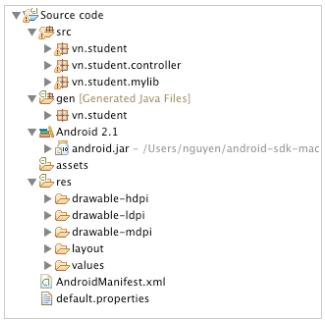
\includegraphics [scale=1] {images/h30.png}
\begin{center}
%\captionsetup{justification=justified, labelsep=period}
\caption{Структура директории и файлов проекта ПО Андроид на Eclipse} \label{img30}
\end{center}
\end{figure}
\textbf{Файл AndroidManifest.xml:}

Этот файл является основой всех Android-приложений, AndroidManifest.xml файл помещается в папке Root и показывает компоненты, которые включены в приложении (activities, services) и как компоненты прикреплены вместе.

При создании файла manifest, необходимо обеспечить свойства пакета, то есть имя пакета Java, используемого в качестве основы для нашего приложения. После ввода имени пакета и, в случае необходимости, в файле manifest, мы можем сократить, например, с классом "com.yourapp.android.search. Someclass", просто пишется: ".Someclass".
\begin{figure}[ht!]
\centering
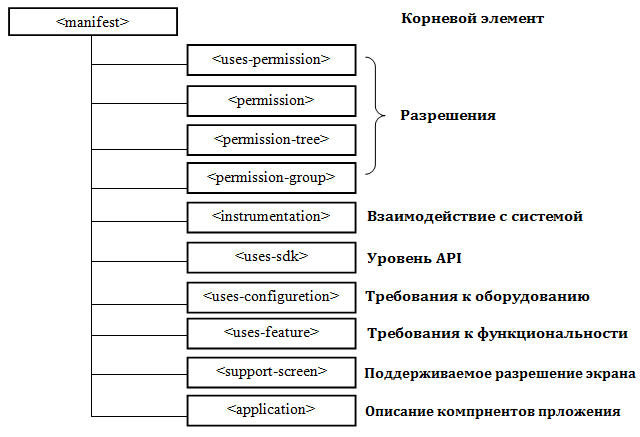
\includegraphics [scale=1] {images/h34.png}
\begin{center}
%\captionsetup{justification=justified, labelsep=period}
\caption{Структура файла Manifest.} \label{img34}
\end{center}
\end{figure}

\subsection{Библиотеки поддержки для разработки приложений}
\textbf{Библиотека обработки изображений для Android – OpenCV}

OpenCV (Open Computer Vision Library) - библиотека компьютерного зрения, которая распространяется в виде открытого исходного кода. Изначально OpenCV была написана для программ на языке C, но теперь работает на других языках, таких как C ++, Java, Android, IOS. А так же время поддерживает много ОС: Windows, Linux, Android, Mac OS, Cube.

В настоящее время в библиотеке OpenCV существует более 2500 алгоритмов, которые включают в себя совокупность всех алгоритмов компьютерного зрения и машинного обучения. Эти алгоритмы могут быть использованы для обнаружения и распознавания лиц, распознавания объектов и классификации человеческих действий в видео, отслеживать перемещение объектов, извлекать 3D модели объектов, нахождения похожих изображений из базы данных изображений, удаления эффекта красных глаз из изображений, снятых с использованием вспышки, отслеживания движения глаз и т.д.

Структура OpenCV включает в себя 4 основных компонента:
\begin{figure}[ht!]
\centering
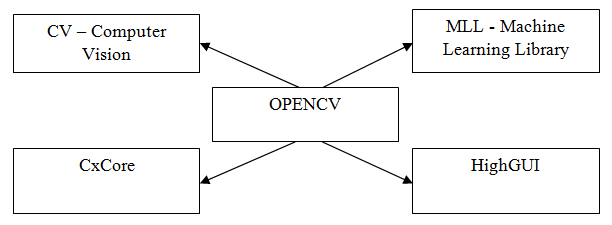
\includegraphics [scale=1] {images/h31.png}
\begin{center}
%\captionsetup{justification=justified, labelsep=period}
\caption{Структура OpenCV} \label{img31}
\end{center}
\end{figure}


\begin{itemize}
	\item \textbf{CxCore}: Содержит основную структуру, такие как точки, линии, блоки, руки, матриц, и связанные с ними манипуляции низкого уровня;
	\item \textbf{MLL} (Machine Learning Library) является библиотекой машинного обучения, эта библиотека включает в себя много классов статистики и инструментов обработки;
	\item \textbf{CV} (Computer Vision – компьютерное зрение): Содержит множество операций, связанных с обработкой изображений низкого уровня, таких как фильтрация изображений, обнаружение контура, преобразование Фурье и прочее;
	\item \textbf{HighGUI}: Работа с файлами изображений и видео, такие как загрузка изображения, отображения изображений, преобразование форматов.
\end{itemize}
\textbf{Open CV имеет следующие основные модули}:

\begin{itemize}
	\item Opencv core: основная функциональность. Включает в себя базовые структуры, вычисления, ввод и вывод для XML и т.д;
	\item Opencv imgproc: обработка изображений;
	\item Opencv highgui: модуль для создания пользовательского интерфейса;
	\item Opencv feature2d: распознавание и описание плоских примитивов (SURF, FASR и др.);
	\item Opencv video:анализ движения и отслеживание объектов;
	\item Opencv objdetect: обнаружение объектов на изображении;
	\item Opencv ml:модели машинного обучения.	
\end{itemize}

\textbf{Библиотека моделирования 3D – MakeHuman}

MakeHuman - программное обеспечение с открытым исходным кодом, является бесплатным, служит для создания 3D модели человека. MakeHuman прост в использовании и имеет интуитивно понятные параметры, в том числе:

\begin{itemize}
	\item Возраст, пол, рост, вес;
	\item Пропорция тела, форма лица;
	\item Глаза, нос, рот, подбородок, уши, шея ...
	\item Руки, ноги

\end{itemize}

Это приложение разработано с использованием 3D-технологий. Создание начинается с формы человека, а затем преобразуется во множество различных персонажей, в том числе мужчин и женщин. Кроме того, мы можем преобразовать 3D модели из формы ребенка в юношу, взрослого и пожилого человека. Начиная с первой версии, MakeHuman использовало уникальные сетки.  

\textbf{Библиотека поддержки моделирования min3D}
\begin{figure}[ht!]
\centering
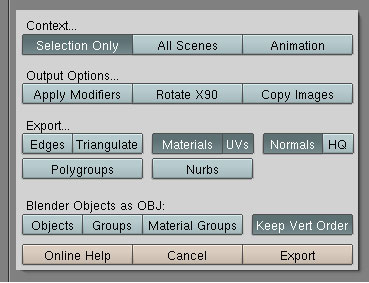
\includegraphics [scale=1] {images/h32.png}
\begin{center}
%\captionsetup{justification=justified, labelsep=period}
\caption{Структура библиотеки моделирования min3D} \label{img32}
\end{center}
\end{figure}

Библиотека Min3D имеет открытый исходный код, разработанный для операционной системы Android для отображения 3D-моделей. Она использует инструмент поддержки OpenGL версий 1.0/1.1. Min3D совместим с OpenGL API, предоставляет удобную и полезную библиотеку для приложений моделирования. Библиотека Min3D легко восстановит 3D-модели объекта. Min3D работает на следующих файлах: Wavefront OBJ, 3DS, MD2.

В данной работе используется сочетание двух библиотек MakeHuman и Min3D для создания шаблонов 3D-моделей человеческого тела. Эти шаблоны описаны в двух файлах с расширениями *.mtl и *.obj. Эти файлы хранятся в папке Андроида (project/res/raw). 


\begin{itemize}
	\item Файлы *.obj содержат данные, описывающие 3D-модели в формате текста, а также другую информацию об объекте. Файлы *.obj просты в использовании и полезны для хранения и отображения 3D-модели любого объекта;
	\item Файлы *.mtl содержат информацию текстур объектов. 
\end{itemize}
Оба файла * .obj и * .mtl являются конечным результатом конструкции 3D-модели человека на основе результата извлечения антропометрических признаков системы компьютерного зрения, предложены библиотека MakeHuman и входные данные для отображения на устройствах Android сгенерированные с помощью библиотеки min3D.





%-------------------------
\section{Программное обеспечение системы компьютерного зрения в антропометрии}
Приложение создано для обработки видео на смартфонах, оно основано на алгоритмах компьютерного зрения в антропометрии с использованием поддержки среды Android и библиотек OpenCV, Min3D, MakeHuman. В данной диссертации применяется система компьютерного зрения в антропометрии для создания приложений в областях пошива одежды (E-Tailor) и фитнеса (E-Fitness). Приложения загружены на онлайн-магазин GooglePlay и их можно скачать бесплатно. Системные требования: версия Android от 4.4.2, передняя камера с разрешением 2.0 мп или выше.

После загрузки и установки, система автоматически загрузит и установит библиотеку OpenCV для телефона.

\input{part3/part3_2_1}
%-------------------------
\input{part3/part3_2_2}
%-------------------------
%-------------------------
\subsection{Основные результаты и выводы по главе 4}

\begin{enumerate}
	\item Описание среды разработки приложения Android, библиотек поддержки алгоритмов компьютерного зрения OpenCV, поддержки построения 3D-моделей человеческого тела MakeHuman и библиотеки поддержки 3D для Android – Min3D;
	\item Описание и инструкция для скачивания программы. Инструкция конфигурации библиотеки OpenCV с Android.
	\item Разработка приложения компьютерного зрения в антропометрии для пошива одежды (E-Tailor). Главные функции: автоматизация извлечения антропометрических признаков и классификация размеров одежды;
	\item Разработка приложения компьютерного зрения в антропометрии для фитнеса (E-Fitness). Главные функции: автоматизация извлечения антропометрических признаков, построение 3D-моделей человеческого тела, анализ и сравнение признаков по телосложению, индексу массы тела (ИМТ);
	\item Приложения разработаны на ОС Android для смартфонов и на основе методов и алгоритмов компьютерного зрения для извлечения и классификации антропометрических признаков. Программный модуль имеет простой, удобный и интуитивно понятный интерфейс.
\end{enumerate}

%-------------------------

\clearpage    % Введение
%\chapter{Примеры применения интегральных уравнений в энергетике} \label{chapt1_intro}
%\chapter{Применения интегральных уравнений в энергетике} \label{chapt1_intro}
\chapter{Аналитический обзор применения методов компьютерного зрения в решении задач антропометрии} \label{chapt1_intro}

В данной главе представлен аналитический обзор алгоритмов и методов компьютерного зрения в антропометрии на основе анализа статических изображениях и видео в режиме, бликом к реальному времени. Приведены их преимущества и недостатки. Рассматривается возможности использования методов и алгоритмов компьютерного зрения для извлечения признаков.

% \section{Пример из моделирования развивающихся динамических систем} \label{sect3_2}
\todo[inline,color=cyan]{Вставить абзац связи АНТРОПОМЕТРИИ с МЗ. Иначе не понятно, что это вы тут распинаетесь по поводу МЗ. Пусть этот абзац будет пропедевтическим.}

\section{Задачи и развитие систем машинного зрения} \label{chapter1.1}

\mrk{МЗ и его краткая история}\emph{Машинное зрение}(МЗ) -- это междисциплинария область\cEA{А нормальное определение есть?}, получившая в настоящее время широкое развитие. Концепция обработки изображений и МЗ является важным разделом компьютерного зрения и основана на комбинации многих дисциплин. Прогресс в области компьютерного зрения определяется развитием математической теории\cEA{Теорией чего?}, численных методов, а также развитием вычислительных ресурсов, в частности, аппаратного обеспечения\cEA{?смартфонов?}. Долгое время теоретические исследования в области МЗ опережали вычислительные возможности ЭВМ, что затрудняло их использование для решения практических задач. В \cite{Paragios2008} условно выделен ряд этапов развития средств зрения МЗ и отмечено, что только с 1970-х годов XX века появилась возможность обрабатывать большие наборы данных. С тех пор концепции и методы МЗ привлекают все большее внимание.

\mrk{Структура МЗ.}
Системы МЗ включают\cEA{Можно добавить картинку-архитектуру} в себя следующие основные компоненты \cite{Rosenfeld2000}:
\begin{itemize}
	\item Подсистему формирования изображений, которая сама, как правило, включает разные компоненты, например, оптическую систему, осветщение и ПЗС- или КМОП-матрицу;
	\item Вычислитель;
	\item Алгоритмы анализа изображений, которые могут реализовываться программно на процессорах общего назначения, аппаратно в структуре вычислителя и даже аппаратно в рамках подсистемы формирования изображений.
\end{itemize}

\mrk{МЗ - важнейший источник информации для ИИ. Приложения.}
МЗ предоставляет важнейшую информацию для создания систем искусственного интеллекта. Такие системы могут получать информацию как из полученных  изображений так и из наборов многомерных данных различной природы \cite{Fan2013}. Сочетание машинного зрения с другими областями, такими как: информационные технологии, связь, электроника, автоматическое управление и т.д. дает нам множество применений в области науки, безопасности, военной , медицины, промышленных роботов и т.д.

\mrk{Применение МЗ -- повторение}
В последние годы проводятся научно-исследовательские работы в различных областях обработки и распознавания изображений. Машинное зрение стало самостоятельной дисциплиной \cite{Huang1991, Kevin1991}. В настоящее время методы машинного зрения реализованы во множестве устройств, применяются технологии обработки и управления, на основе изображения. Приведем краткий обзор приложений систем машинного зрения в робототехнике.

\subsection{Машинное зрение в робототехнике}

\mrk{Структура МЗ роботов и решаемые задачи.}
Система МЗ роботов является интегрированной системой, включающей одну или несколько камер \cite{Abebe2016}. В зависимости от назначения, система должна обнаруживать положение объектов в поле зрения камеры (ROI, Region of Interest). На основе этой системы, робот решает задачи определения местоположения и направления движения объектов. Для достижения высокой эффективности\cEA{Критерии эффективности? Или ж речь идет о режиме реального времени} работы необходимо обеспечивать эффективную совместную работу системы, включая аппаратные средства и программное обеспечение \cite{Zhu2004, Vayda1991}.

\mrk{Применение МЗ в промышленности.}
В современной промышленности системы компьютерного зрения роботов применяется в различных областях, таких как:
\begin{itemize}
	\item автомобильная промышленность с автоматизированными системами сборки и обработки двигателей, автомобильных кузовов;
	\item пищевая промышленность, например, система контроля автоматического закрывания пакета, закрывания контейнера  обнаружения посторонних предметов в пище при упаковке;
	\item фармацевтическая промышленность: контроль упаковки и партии, обнаружение дефектов;
	\item военно-силовые структуры: обнаружение целей беспилотными летательными аппаратами, анализ багажа, анализ поведения групп людей в общественных местах.
	\item обеспечение безопасности, предупреждение преступности в том числе \cEA{Распознавание чего делается? -- много неопределенности}на основе антропометрических признаков;
	\item индустрии развлечений и спорта: системы автоматического управления камерой слежения за объектами в футбольном матче, гонках и т.д.
\end{itemize}

\mrk{Классы задач МЗ в робототехнике.}
Таким образом, современная робототехника требует решения многих сложных задач МЗ, в том числе следующих:
\begin{itemize}
	\item ориентация во пространстве и определение расстояний до объектов;
	\item распознавание и классификации различных объектов, интерпретации сцен, навигация;
	\item обнаружение людей, распознавание их лиц и анализ эмоций;
	\item восстановление изображений и подавление шумов, повышение разрешнения изображений, в том числе получение изображений со сверхразрешением.
\end{itemize}

\subsection{Машинное обучение и информационный поиск}

\todo[inline]{Связь МЗ и машинного обучения}

\mrk{Машинное обучение и интернет-проекты}
На сегодняшний день машинное обучение используется в бесчисленном множестве интернет-проектов. У многих известных IT-компаний (к примеру, Яндекс, Google, Facebook, Microsoft) на нём базируются многие ключевые технологии \cite{Cormier2016}.

\mrk{Поиск, сравнение и классификация изображений в Интернет}
Задачи поиска изображений по содержанию также разнообразны. Они включают в себя следующие шаги \cite{Meer2000}. Сравнение содержимого изображения для обнаружения и распознавания на изображениях объектов классов\cEA{Не слищком абстрактно?} разной степени общности. Такие алгоритмы очень полезны для создания приложений, таких как: классификация данных (изображения, видео и т.д.), поиск товаров на основе изображений для интернет-магазинов, для извлечения изображений в геоинформационных системах, для систем биометрической идентификации, для специализированного поиска изображений в социальных сетях (например, для поиска лиц людей, привлекательных для пользователя) \cite{Findface} и т.д., вплоть до поиска изображений в интернете.

\mrk{МЗ-задачи решаются методами машинного обучения. -- хороший кандидат на первый абзац раздела.}
Методами машинного обучения при разработке систем компьютерного зрения решаются проблемы распознавания объектов. Разработка алгоритмов классификации является одной из важнейших областей машинного обучения \cite{Murino2000}. Методы глубокого обучения (deep learning) требуют огромных вычислительных ресурсов, и даже для обучения распознаванию ограниченного класса объектов могут требоваться несколько дней работы на вычислительном кластере. При этом в будущем могут быть разработаны еще более мощные, но требующие еще больших вычислительных ресурсов методы.  Отметим, что использование специфики решаемой задачи позволяет существенно сократить вычислительную сложность, однако требует более глубокого понимания сути решаемой задачи.

\todo[inline,color=cyan]{Ну и какая СОДЕРЖАТЕЛЬНО ПРЕДСТАВЛЕННАЯ связь М-обучения с МЗ и приложениями на производстве и робототехнике, кроме специфики задачи???}

\subsection{Мобильные приложения машинного зрения}

\mrk{МЗ на моб.устройствах. Фичи мобил}
Задачи компьютерного зрения все шире используются в приложениях для персональных мобильных устройств, таких как смартфоны, планшеты и прочее. В частности, число смартфонов неуклонно растет и уже практически превысило по численности население земли \cite{Battiato2012}. Часть задач по обработке изображений для мобильных устройств с камерами совпадает с задачами для цифровых фотоаппаратов. Основное отличие заключается в качестве объективов и в условиях съемки. В спектре аппаратного обеспечения, доступного для решения задач отметим модули с доступом к интернет, наличия интернета, GPS и конечно мощного процессора и большой памяти. Именно с этим связано появление такого термина, как <<smart phone>> \cite{Hannuksela2007}.

\mrk{???? + МЗ+Дополненная реальность....???}
В этой связи решение, казалось бы, идентичных задач для разных устройств может различаться, что делает эти решения высоко востребованными на рынке. Приложения для смартфонов выходят на рынок, наблюдается огромный интерес к компьютерному зрению и приложений дополненной реальности в мобильных устройствах \cite{Shubina2010}.

\mrk{Примеры задач МЗ на мобилах}
В настоящее время существует много приложений, использующих обработку изображений, для мобильных устройств. Например, программа автоматической коррекции лицевых дефектов (таких, как морщины, угри, веснушки) в соответствии с заданным стилем (натуральный, классический, контраст и т.д.). Это такие приложения, как camera360, Perfect Selfie. Приложения по обработке изображений на видео позволяют пользователям создавать тематические видео из фотографий, анимации и т.д. -- MiniMovie, Imovie-editing и Маскарад, которые преобразует видео в стиль картин художника Ван Гога и мультипликации.

\mrk{Задачи ориентации, распознавание кепоинтов. ДОПИСАТЬ ПРИМЕРЫ.}
Более сложные задачи, связанные с сопоставлением (отождествлением сопряженных точек) на изображениях, оценкой трехмерной структуры сцены, определением изменения ориентации камеры, распознавание объектов, а также анализа лиц людей, также находят свои приложения в\ldots{}\cEA{Привезти примеры.}. Повышение качества решения перечисленных задач требует совершенствования и разработки нового математического и программного обеспечения, и адаптации его к вычислительным возможностям мобильных устройств, а также к их периферии.

\mrk{Резюме - МЗ на мобилах - это круто.}
Перечисленные примеры и задачи показывают, что класс приложений МЗ на мобильных устройствах крайне широк и любое продвижение в развитии и исследовании методов обработки изображений является актуальным.
\todo[inline,color=cyan]{Какая связь СОДЕРЖАНИЯ РАЗДЕЛА с АТРОПОМЕТРИЕЙ?}

%%% Local Variables:
%%% mode: latex
%%% TeX-master: "../dissertation"
%%% End:

%-------------------------
\section{Анализ алгоритмов и методов компьютерного зрения для извлечения признаков в антропометрии}

Использование современных методов компьютерного зрения позволяет разрабатывать новые подходы к автоматизации различных адач антропометрии. Компьютерное зрение предоставяляет большой арсенал методов для решения задач антропометрии. Условно такие задачи можно разбить на следующие этапы: калибровка, регистрация изображения (или видео), обнаружение объекта (человека), сегментация и выделение признаков (антропометрических измерений). Дополнительно может понадобиться классификация признаков и  построение 3D модели человека (это будет рассмотрено ниже) \cite{Rebak2016}.

\subsection{Антропометрические признаки}

Изображение представлено матрицей пикселей. Изображение содержит различные функции, это зависит от содержания каждого изображения. Исходя из нашей цели необходимо реализовать алгоритмы извлечения признаков, чтобы достичь наилучшей точности, устойчивости и скорости антропометрии.

Итак, первая задача состоит в использовании и преобразовании изображения в вектор признаков. По сути это представление информации в более сжатом виде в зависимости от решаемой задачи. 

Признак (feature)  $f$  объекта $a$ – отображение $f:A\rightarrow D_f$  где $D_f$ – множество допустимых значений признака \cite{Mecte2002}.  Если имеется набор признаков $f_1,…,f_n$, то вектор $x= \left(f_1\left(a\right), ..., f_n\left(a\right)\right)$ называется признаковым описанием объекта $a\in A$. Признаковые описания с определенными ограничениями допустимо отождествлять с самими объектами. При этом множество $A=\left(D_{f_1}\times ... \times D_{f_n}\right)$ называют признаковым пространством (feature space, пространство признаков). Задаче извлечения признаков объектов, как правило, предшедствуют этапы обнаружения и сегментации объектов. 
Антропометрические признаки выражены в форме и размерах частей человеческого тела (рис. \ref{img1}).
\begin{figure}[htb]
\centering
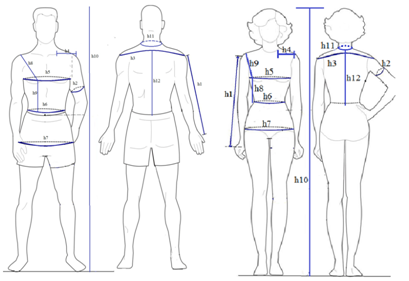
\includegraphics [scale=0.8] {images/h1.png}
\begin{center}
%\captionsetup{justification=justified, labelsep=period}
\caption{Описание антропометрических признаков.} \label{img1}
\end{center}
\end{figure}

Признаки формы. Форма объекта или области является важной характеристикой при обнаружении и классификации изображений в распознавании образов \cite{Jones2002}, \cite{Dubinskiy2003}. Основная цель анализа формы состоит в измерении геометрических свойств объекта, используемых в классификации, сравнения и распознавания объектов \cite{Kpalma2006}. Так, в области антропометрии, антрометрической характеристикой является размер частей человеческого тела. Он состоит из следующих величин \cite{urlclothes2015}: рост, длина рук, длина ног, окружность талии, окружность грудной клетки, окружность бедер и т.д. Современные антропометрические измерения могут служить основой для 3D моделей человеческого тела\cite{Toldo2009}, \cite{Ponce1989}, \cite{Zhang2001}.

Использование цвета кожи в ввиде признаков. Цвет является отличительной особенностью и используется для алгоритма обнаружения кожи \cite{Fink2006}. Каждый пиксель (информация о цвете) может быть представлен в виде трехмерной точки в определенном цветовом пространстве \cite{Albio2001}, \cite{Shin2002}. Общие цветовые пространства: RGB, Munsell, CIE, HSV \cite{Jones2002}.

\subsection{Извлечение антропометрических признаков}

Приведем краткий обзор исследований, посвященных применению методов компьютерного зрения к решению задач антропометрии, анализу положений человека и создания 3D-моделей. Для статических изображений было сделано несколько научно-исследовательских работ для того, чтобы обнаружить человеческое тело, используя описание фона и модели человеческого тела \cite{Mori2002}. В \cite{Belongie2002} представлен алгоритм сегментации частей тела на основе силуэта. Данный подход делит тело на основе использования контура каждой области на теле человека. Авторы отмечают, что их алгоритм выполняется плохо, когда части тела, особенно руки, держатся близко к телу. Авторы \cite{Mittal2003} продемонстрировали, что использование искусственно сгенерированных данных обучения помогает произвести сегментацию человеческого контура, взятого из шумных изображений реального силуэта. Авторы утверждают, что такая сегментация должна хорошо работать, несмотря на шум в исходных данных.

Извлечение антропометрических признаков выбирается на основе 2D-изображений. Оно предоставляет данные для многих приложений. Например: бесконтактное измерение размеров человеческого тела \cite{Lin2008}, построение 3D моделей \cite{Lin2010}, \cite{Lin2012}, распознавание человеческих действий \cite{Ikizler2008}. 
В работе \cite{Gopal} предложена методика сочетания наборов данных (PCD) для синтеза антропометрических баз данных на основе легкодоступной информации о значениях измерения различных областей человеческого тела. Авторы собрали такие данные для улучшения анализа перемены населения. Метод состоит из трех этапов: сбор описательной статистики о антропометрии, подгонка антропометрических моделей к этой информации, а также формирование антропометрической модели для генерации необходимых данных. Применение этой процедуры продемонстрировано на двух базах данных: военных США в конце 1980-х и японской молодежи в начале 1990-х годов. Методика является простой, легко применимой и точной. В данной статье \cite{Adams} представлен количественный анализ качества данных, собранных в ходе опроса населения волонтерами.  В результате обследования населения были получены данные артериального давления и антропометрии. На протяжении всего исследования собраны антропометрические данные и кровяное давление, которые были в пределах допуска для ошибок, установленных в начале исследования. В статье \cite{Jiang2012} предлагается подход для автоматического обнаружения ключевых точек контура человеческого тела. Этот метод применяется к изображениям, в которых имеется две раличные  позы (стоя в профиль и анфас). Реализуется он следующим образом: во-первых, используется эффективный подход к обнаружению формы тела - метод на основе обнаружения края \cite{Canny1986} и 8-связного цепного кода Фримэна \cite{Freeman1961}. Затем определяются взаимосвязанные регионы. Ряд характерных точек извлекается на основании указанных правил путем измерения разности между областями сегментов. В общей сложности 101 характерная точка с четкими геометрическими свойствами извлекаются автоматически, в том числе 27 точек, соответствующих определений ориентиров об измерениях швейной индустрии. Наконец, предлагаемый подход был протестирован на человеческих субъектах, и целых 101 характерных точек с конкретными геометрическими характеристиками были правильно извлечены, что свидетельствует об эффективной и надежной работы (рис. \ref{img2}).

\begin{figure}[ht!]
\centering
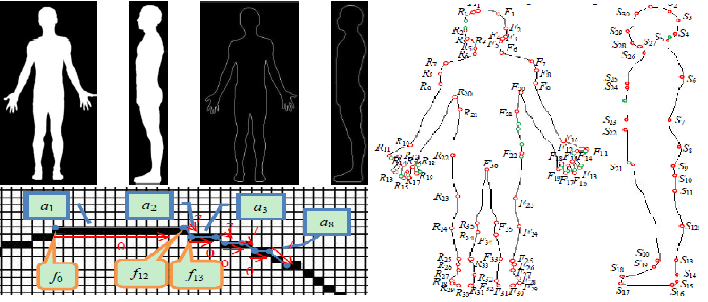
\includegraphics [scale=0.8] {images/h2.png}
\begin{center}
%\captionsetup{justification=justified, labelsep=period}
\caption{Маркировка контура в методе извлечения антропометрических признаков на основе ключевых точек \cite{Lin2008}.} \label{img2}
\end{center}
\end{figure}

В работе \cite{Nevatia2009} предложен метод обнаружения объектов в случае их частичной видимости в поле зрения. Метод апробирован на видеопотоке уличных сцен. Основной вклад этого метода включает:

\begin{itemize}
	\item Проектирование иерархии для процесса обучения путем деления признаков;
	\item Метод сегментации объектов на основе  классификатора AdaBoost.
\end{itemize}

Ioffe и Forsyth \cite{Ioffe2001} предложили методы автоматизации антропометрии, основанные на обнаружении частей тела человека. Их система подразумевает, что человек одет в специальную одежду. Определения сегментов для определения ключевых точек тела, необходимых для правильного измерения длины сегментов тела встречаются в \cite{Leva1996}. 

\begin{figure}[ht!]
\centering
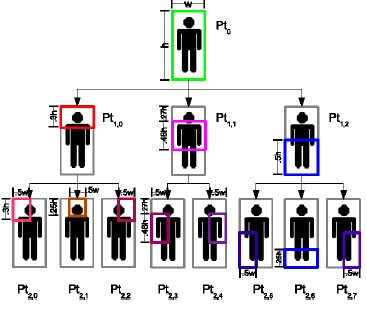
\includegraphics [scale=0.8] {images/h3.png}
\begin{center}
%\captionsetup{justification=justified, labelsep=period}
\caption{Описание системы обнаружения объекта на основе обнаружения каждой его части \cite{Nevatia2009}.} \label{img3}
\end{center}
\end{figure}

На (рис. \ref{img3}) представлена часть обнаружения тела человека на основе каскадных признаков и метода классификации на основе boosting. Программа включает в себя 3 этапа: 1) обнаружение человека, 2) обнаружение верхней части тела, средней и нижней частей тела, 3) соотнесение различных частей человеческого тела. Используется следующая классификация : верхняя часть тела (голова, правая, левая часть лица), средняя часть тела (правая рука, левая рука), нижняя часть тела (правая нога, левая нога, ноги). 

Кроме того, улучшен метод, использующий математические модели формы (3D-сканирование) для извлечения антропометрических признаков. В \cite{Baek2012} авторы предложили построение модели, которая состоит из трех основных этапов: построение базы данных, статистического анализа и генерации модели. База данных была собрана из 250 3D-сканов всего тела. Данные обрабатываются, чтобы сделать ввод данных для статистического анализа (рис. \ref{img4}). Используется соотношение частей человеческого тела для построения 3D модели. Система определяет местоположение и форму каждой части тела и вычисляет её размер. По сравнению с другими параметрическими методами моделирования человека \cite{Siebert2000}, \cite{Seo2001}, их метод вносит свой вклад путем введения нового способа соотношения формы и размеров тела путем создания усовершенствованной техники оптимизации параметров для генерации математической модели тела человека.

\begin{figure}[ht!]
\centering
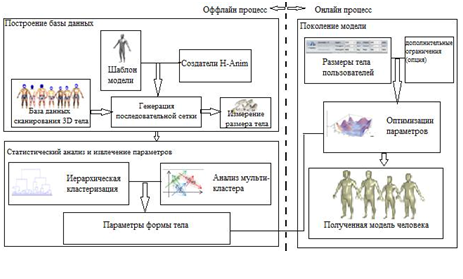
\includegraphics [scale=0.8] {images/h4.png}
\begin{center}
%\captionsetup{justification=justified, labelsep=period}
\caption{Описание метода извлечения антропометрических признаков на основе сканирования тела \cite{Baek2012}} \label{img4}
\end{center}
\end{figure}

Авторы в работе \cite{Blanz1999} также предложили метод математического моделирования формы человеческого тела. Система собирает данные путем 3D сканирования человеческого лица. Система анализирует полученные данные на основе основного метода главных компонент - PCA. Используя эту специальную базу данных, можно проанализировать и извлечь доминирующие переменные, определяющие форму лица. Используя идеи статьи \cite{Blanz1999}, Allen \cite{Allen2003} установил набор 3D данных сканирования тела. Был разработан новый способ генерации последовательной структуры сетки путем аппроксимации на основе шаблонов. В \cite{Seo2003}, \cite{Seo2004} авторы предложили использовать нейросетвой подход в этой задаче. Этот подход показал высокую эффективность для соотнесения размера фактического человеческого тела с размером тела базы данных. Критическую роль в этом подходе играет процесс обучения. Была обнаружена зависимость между формой и размерами человеческого тела. На основе этих отношений, система синтезирует новую модель с размером тела путем сопоставления формы в базе данных. Стандартные сканеры обычно используют бинарные модели, состоящие из черных и белых полос.  Этот подход подвержен ошибкам из-за зависит от разрешения и шума \cite{Rocchini2001}. Кроме того, это также зависит от расстояния между объектом и устройством. Это влияет на результаты восстановления изображения на основе данных, которые получены со сканера. Система работает эффективно даже в условиях низкой освещенности. Другой подход, основанный на компьютерном зрении изложен в работе \cite{Taeyoung2015}. Система состоит из четырех основных этапов: обработки изображений на основе вычитания фона и распознавания маркера, обработки инфракрасных изображений для надежного обнаружения маркера, для проектирования ортопедических стелек с учетом индивидуальных особенностей (рис. \ref{img5}).

\begin{figure}[ht!]
\centering
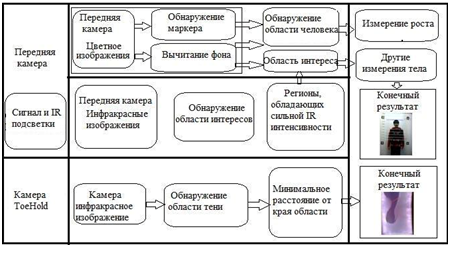
\includegraphics [scale=0.8] {images/h5.png}
\begin{center}
%\captionsetup{justification=justified, labelsep=period}
\caption{Описание системы извлечения антропометрических признаков в остеопатии\cite{Taeyoung2015}.} \label{img5}
\end{center}
\end{figure}

Эта тема получила развитие в работах \cite{McCulloch1988} и \cite{Lee2000}.

%-------------------------
\section{Анализ методов машинного обучения для классификации признаков}

В настоящее время существует множество методов и алгоритмов компьютерного зрения, предложеных и развитых для классификации данных.

Особенности систем машинного зрения позволяют вырабатывать требования для разработки методов и алгоритмов классификации. Кроме того, тип данных является решающим фактором адекватности и точности классификации \cite{segi1998}, \cite{sophi2000}. Было много исследований в которых успешно применяются алгоритмы и методы компьютерного зрения для классификации данных, таких как распознавание жестов \cite{Phan2013}, распознавание лиц \cite{Phakhi2013, Goldstein1991}, идентификация деятельности человека \cite{Kang2006, Saaidi2008}. Адаптивные методы распознавания объектов и классификации основаны на автоматической подстройке к свойствам обрабатываемых данных, что позволяет разработать распознающую систему с приемлемыми характеристиками \cite{anwef2011}. Ко второй категории относятся методы, характеризующиеся сокращением размерности данных \cite{Belhumeur1997}, \cite{Hallinan1999}. Ниже изложим наиболее популярные методы классификации.

\subsection{Алгоритм AdaBoost}

Алгоритм AdaBoost был разработан Йоавом Фройндом (Yoav Freund) и Робертом Шапиром (Robert Schapire) в 1996 году \cite{Freund1997}, \cite{Freund1996}. Этот алгоритм <<адаптивность и усиление>> используется для создания классификатора. Как известно, классификатор на входе принимает набор данных для обучения и пытается предсказать или классифицировать новые образцы данных, которые относятся к определенному классу \cite{Sochman2004} (рис. \ref{img6}). Алгоритм AdaBoost построен на основе алгоритмов обучения (например, деревья решений) и объединения их. Цель состоит в том, чтобы создать один сильный классификатор на основе нескольких слабых классификаторов. Алгоритм AdaBoost успешен в поиске личной информации на статических изображениях \cite{Su2005}. Сайты постоянно поддерживают поиск информации на основе изображений используя AdaBoost.

Система поиска лица на основе алгоритма <<Viola-Jones>> \cite{Viola2001}, \cite{Violaj2001} также использует AdaBoost. Эти системы работают с высокой точностью, например в цифровых фотокамерах и смартфонах. Вейвлет Хаара \cite{Viola2004} являются одним из простых признаков, которые обычно используется на практике. Но размер такого вектора-признака довольно большой (162,336). Таким образом, нужно применять метод главных компонентов (англ. principal component analysis, PCA) \cite{Masoud2005} для увеличения или уменьшения размера и выбора новых функций. После этого полученные данные классифицируются алгоритмом AdaBoost.


\begin{figure}[ht!]
\centering
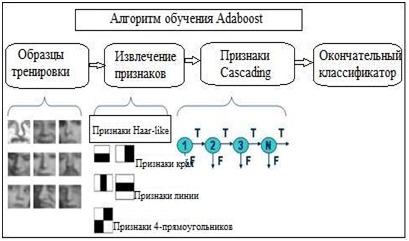
\includegraphics [scale=0.8] {images/h6.png}
\begin{center}
%\captionsetup{justification=justified, labelsep=period}
\caption{Описание алгоритма AdaBoost \cite{Sochman2004}.} \label{img6}
\end{center}
\end{figure}

Этот алгоритм прост и удобен а также, имеет очень высокую скорость обучения.  Алгоритм AdaBoost гибкий и универсальный, может быть объединен с любым алгоритмом машинного обучения, и может работать с большим количеством различных данных.

\subsection{Искусственные нейронные сети}

Нейронная сеть была успешно использована для решения задач классификации объекта \cite{Hinton2012}. С точки зрения машинного обучения, искусственные нейронные сети (ИНС) являются вычислительными моделями, которые способны решать задачи распознавания образов \cite{Sergios2006}, \cite{Dunne2007}. Нейронную сетевую архитектуру можно разделить на две основные группы: сети прямой связи \cite{Colin2000} и обратного распространения сети \cite{Kamruzzaman2006}. При решении задачи классификации возраста и пола человека применяется большое количество нейронных сетей различных архитектур \cite{Rowley1998}, в частности: вероятностные нейронные сети (probabilistic decision-based neural networks) \cite{Lin1997}, многослойные персептроны \cite{Juell1996} и т.д. Нейронные сеть - ИНС являются одним из приоритетных направлений исследований в области машинного обучения.

Действительно, искуственные нейронные сети способны решить различные проблемы: классификация образов, аппроксимации функций, оптимизация и квантование вектора пространства данных, в то время как традиционные методы не могут эффективно решить вышеуказанные проблемы.

\subsection{Метод опорных векторов}

Метод опорных векторов (Support Vector Machines, МОВ)  используется для решения задач классификации и регрессионного анализа. Этот метод был предложен В. Вапником и А. Червоненкисом в 1995 году \cite{Vapnik1995}. Особые свойства МОВ – это непрерывное уменьшение эмпирической ошибки классификации. Использование МОВ и мешка признаков (Bag-of-Features) оказалось эффективным в задачах обнаружения и распознавания жестов на видеопоследовательности \cite{Nasser2011, Dardas2010}, а также при решении других задач \cite{Jiang2007, Lazebnik2006}. Метод опорных векторов (МОВ) позволил классифицировать нормальные и ненормальные поведения человека \cite{Yogameena2010}. В работе \cite{Nguyen2015} авторы представили предлагаемый подход к классификации пола и размера одежды с помощью метода опорных векторов. Алгоритм работал с антропометрическими данными для классификации по двум классам: мужчины / женщины.

Метод опорных векторов, как и методы на основе деревьев решений даёт высокую точность для наборов данных с непрерывными типами данных (непрерывное значение). Они являются двумя методами, которые обычно используются для классификации данных. Тем не менее, не существует универсального метода классификации. Результат всегда зависит от цели системы и типов данных. Кроме того, выбор ядра и других параметров является  слабостю МОВ.

\subsection{Алгоритм случайного леса (Random Forest)}

Random Forest (случайный лес) \cite{Breiman2002, Breiman2001} является развитием семейства алгоритмов, разработанных Лео Брейман в университете Калифорнии, Беркли. На самом деле, Random Forest использует методы, называемые мешки (bagging). Эта методика позволяет выбрать подмножество атрибутов в каждом узле дерева классификатора, чтобы разделить его на следующий уровень. Таким образом, Random Forest имеет возможность разделить очень большое пространство поиска на меньшие пространства поиска. Таким образом, алгоритм может выполнять сортировки быстро и легко.

В случайном лесе, разработка набора деревьев значительно улучшила точность классификации, каждое дерево в наборе будет <<голосовать>> за самый популярный класс. Для развития наборов деревьев, как обычно, создаются случайные векторы. Такие векторы будут регулировать развитие каждого дерева в вышеупомянутом наборе. Для дерева $K$ в наборе, случайный вектор $\theta_k$  генерируется, независимый с генерированными векторами ранее $\theta_1, \theta_2, ..., \theta_{k-1}$, но распределение таких векторов одинаково. 

Дерево было разработано на основе обучающего множества и вектора $\theta_k$. Получается результат: подкласс $h\left(x, \theta_k \right)$ где $х$ - входной вектор. После создания большого количества деревьев, проводится голосование <<голосовать>> за самый популярный класс.

Случайный лес определяется следующим образом \cite{Biggio2011}: подкласс случайного леса, состоящий из наборов слоистой структуры дерева $\left\{h\left(x,\theta_k\right), k=1, ...,n\right\}$ где $\left\{\theta_k\right\}$- независимые векторы, также случайным образом распределенные, и каждое дерево даёт один голос для наиболее популярного класса в входном векторе $х$.

Основная идея алгоритма случайного леса:

\begin{itemize}
	\item В каждом подразделении деревьев, случайный набор m атрибутов взят из m таких атрибутов, которые участвуют в распределении деревьев;
	\item -	Первый шаг в оценке важности переменной в тренировочном наборе – тренировка случайного леса в этом наборе. Во время процесса построения модели для каждого элемента тренировочного набора считаются так называемой <<out-of-bag>> ошибкой. Затем для каждой сущности такая ошибка усредняется по всему случайному лесу.
\end{itemize}

По алгоритмам Random Forest (случайного леса) отметили, что случайный лес является хорошим методом классификации, потому что: 1) в методе Random Forest, ошибки были сведены к минимуму в результате случайного леса, синтезированию через обучения (learner), 2) случайный выбор на каждом этапе в Random Forest снизит корреляцию между учащимися в синтезе результатов. Кроме того, мы также обнаружили, что общая ошибка из слоистых лесных деревьев зависит от их индивидуальных ошибок в лесных деревьях, а также корреляции между деревьями.
%-------------------------
\section{Приложение компьютерного зрения в антропометрии}

Применение методов компьютерного зрения в антропометрии должны соответствовать следующим требованиям: быстрая скорость обработки, высокая точность, возможность создать базу данных для создания приложений на практике. Для приложений безопасности, например, используется программное обеспечение распознавания объектов на основе антропометрических признаков лиц \cite{Graham1997}, 3D моделирование \cite{Zouhour2006} для областях тестильной промышленности, здоровья. Сканеры тела все чаще используются для оценки состояния здоровья и антропометрии, напримеры Caesar project \cite{Robinette2006}, SizeUK \cite{Uk2013} and SizeUSA \cite{Usa2013}. В будущем такие системы будет развиваться для решения различных задач антропометрии.

BreuckmannBodySCAN \cite{Hexagon2016} - это система для проведения антропометрических измерений. По сравнению с ручным измерением, антропометрическое измерение демонстрирует незначительную погрешность. Однако это показывает, что автоматические антропометрические измерения, сравнимо лучше традиционного метода - вручную. Для проверки ошибок авторы используют систему на основе так называемого соотношения значительного/границы (significant/borderline). Если коэффициент > 0.9, то результат измерения является приемлемым. Преимущество этой системы состоит в том, что она не зависит от движения объекта или отсутствия движения объекта, не подверженных внешним факторам, таких как шум и т.д.

3DscannerData \cite{Sobota2009} является приложением, в котором система компьютерного зрения используется в области медицины. Система анализирует форму человеческого тела. Система позволяет проводить ряд антропометрических измерений на основе данных со сканера человеческого тела. Система позволяет анализировать и прогнозировать жир в организме человека. Системы, основанные на размере тела, по сравнению со стандартным размером, чтобы выяснить разницу. Недостатком этой системы является то, что нельзя определить точное местоположение ключевых точке на теле человека для проведения антропометрических измерений. Для повышения точности системы, авторы улучшили алгоритм обнаружения позиций учета каждой части тела. Преимущества вычислительной системы заключается в быстрой работе и не нуждается во вмешательстве  пользователя.

Некоторые интеллектуальные системы на основе компьютерного зрения были применены в текстильной промышленности. Среди них, уже существующих систем были использованы непосредственно для изготовления одежды на заказ. Поэтому, в рамках диссертации предлагается система, которая, например, может помочь портному (или сотруднику фитнес-центра) измерить размеры тела клиента автоматически. Эта система использует способ и систему, основанную на  компьютерном зрении, обеспечивая комфорт и конфиденциальность для клиентов и в целях экономии средств и удобств для заказчика такого антропометрического измерения. С помощью экспериментов, система доказала, что имеет возможность измерить размеры частей человеческого тела быстро и качественно, даже при наличии шума в исходных данных. Таким образом, система автоматического измерения человеческого тела на основе компьютерного зрения представяляет интерес в различных областях, включая швейную промышленность.

Кроме того, эта система может применяться в области фитнеса. Система помогает пользователям часто проводить антропометрическое измерение, проверкять индекс ожирения, выдавая в результате. Таким образом, работы состоит в том, чтобы на основе методов компьютерного зрения создать приложение для смартфонов для решения задач антропометрии.
%-------------------------
\section{Цель и задачи исследования}

Система компьютерного зрения в антропометрии для смартфонов включает следующие три основных этапа:
\begin{itemize}
	\item Первый этап: извлечение антропометрических признаков и создание векторов антропометрических признаков;
	\item Второй этап: классификация данных антропометрических признаков на основе данных из векторов признаков;
	\item Третий этап: Создание приложений для смартфонов на базе результатов классификации.
\end{itemize}

В данной работе осуществляется разработка алгоритмов, методов компьютерного зрения для извлечения признаков и классификации данных в статических изображениях и видео в режиме реального времени. Она актуальна из-за необходимости создания систем компьютерного зрения, которые имеют лучшую эффективность, высокую скорость обработки данных для смартфонов. Система должна соответствовать условиям работы в среде шумов и в реальном времени. Развитие этого направления может быть использовано для создания интеллектуальных приложений в областях моды, красоты, фитнеса, анализа биомедицинских изображений.

Целью диссертации является разработка алгоритмов, методов компьютерного зрения в извлечении признаков и классификации антропометрических данных для построения зрительной системы для смартфонов. Эта система используется в условиях шумов и обработки данных статических изображений и видеокадров в реальном времени.

Для достижения этих целей необходимо решить следующие задачи:

\begin{itemize}
	\item Выполнять анализ подходов с использованием алгоритмов, методов компьютерного зрения для извлечения антропометрических признаков с изображений и видеопоследовательностей и предложить наиболее подходящий подход для решения данной задачи;
	\item Исследование и применение методов калибровки для повышения точности сегментации и местонахождения, измерять размеры частей человеческого тела на изображениях и видеопоследовательностях;
	\item Разработка и реализация алгоритмов, программы извлечения и классификации антропометрических данных на основе алгоритмов, методов предложенного компьютерного зрения;
	\item Оценка и редактирование точности результата системы компьютерного зрения в антропометрии;
	\item Разработка приложений компьютерного зрения в антропологии для пошива промышленности и здоровья, фитнеса. Система работает со статическими изображениями и видео в режиме реального времени;
	\item Сравнение результатов зрительной системы в антропометрии с полученными результатами других авторов.
\end{itemize}
%-------------------------
\section{Основные результаты и выводы по главе 1}

\begin{enumerate}
	\item В этой главе анализируются алгоритмический подход, методы компьютерного зрения в извлечении антропометрических признаков со статических изображений и видеопоследовательностей:
	
	\begin{itemize}
		\item Построение признаков ключевых точек из 2D-изображений, видеокадров;
		\item Использование 3D-сканирования моделей и сопоставление точек человеческого тела в построенных моделях.
	\end{itemize}
	
	\item В данной главе анализируется алгоритмический подход, методы компьютерного зрения в классификации антропометрических данных признаков в изображениях и видеопоследовательностях. Включая:
	
	\begin{itemize}
		\item Алгоритм Adaboost;
		\item Нейронные сети;
		\item Опорных векторов (SVM).
	\end{itemize}
\item Также здесь рассматриваются возможности использования алгоритмов ICP и разреза графов (Graph-сuts) для извлечения антропометрических признаков и алгоритм случайного леса для классификации антропометрических данных в изображениях и видеопоследовательностях.
\item На основе проведенного анализа принято решение о адекватности и точности использования комбинированных алгоритмов ICP, разреза графов (Graph-cuts) для извлечения антропометрических признаков с использованием метода случайного леса (Random Forest) для классификации антропометрических данных в статических изображениях, видео в присутствии шума и в режиме реального времени. Такой подход позволяет построить систему компьютерного зрения в антропометрии с высокой точностью и скоростью обработки.
\end{enumerate}

%-------------------------

%%% Local Variables:
%%% mode: latex
%%% TeX-master: "../dissertation"
%%% End:
	% Введение, обзор.
%\chapter{Линейные интегральные уравнения Вольтерра I рода с кусочно-непрерывными ядрами} \label{chapt1}
%\chapter{Интегральные модели Вольтерра на основе линейных уравнений} \label{chapt1}
%\chapter{Интегральные модели развивающихся динамических систем на основе линейных уравнений Вольтерра I рода с разрывными ядрами} \label{chapt1}
\chapter{Развитие методов и алгоритмов компьютерного зрения в антропометрии} \label{chapt1}

В этой главе излагаются принципы решения проблем приложения компьютерного зрения в задаче антропометрии использую статические изображения или видеопоследовательностях в режиме реального времени. Приводится подробное описание алгоритмов и методов, используемых для обнаружения и классификации объектов, извлечения признаков на изображениях и видеопоследовательностях.


\section{Обоснование исследования и приложения алгоритмов компьютерного зрения в антропометрии}

В задаче математического моделирования тела человека на основе бесконтактных антропометрических измерений важнейшую роль играет синтез различных подходов, включая алгоритмы обнаружения объекта, алгоритмы извлечения признаков, алгоритмы классификации объектов. Разработка систем компьютерного зрения в антропометрии является целью данного диссертационного исследования.


Алгоритмы и методы компьютерного зрения являются не только необходимыми для создания системы программного обеспечения, но и для дальнейшего изучения преимуществ каждого алгоритма и метода, составляя теоретическую важность развития данного направления научных исследований. Для достижения высокой эффективности и скорости обработки видеоданных необходимо сочетание с другими алгоритмами. Условием выбора простого алгоритма является быстрая скорость обработки, которая удовлетворяет реальные потребности системы и сохраняет при этом ее точность.

Исследование алгоритмов и методов в области компьютерного зрения требует процесса анализа и оценки преимуществ и недостатков каждого алгоритма и метода. Необходимо четкое понимание структур системных операций, эффективность и точность каждого этапа всей системы. Нужно четко проанализировать систему, чтобы правильно выбрать алгоритм.

Автоматизация процесса извлечения антропометрических признаков (расположение и размер каждой части человеческого тела, как описано на (рис. \ref{img1})) является важным элементом эффективной работы всей системы. Результатом извлечения антропометрических признаков являются входные данные для классификации объектов и создания приложений для смартфонов.

Данные со статических изображений и видео, факторы окружающей среды (ограничения по разрешению камеры и шуму условия регистрации, включая освещение, траекторию и скорость движения камеры и пр.) будут влиять на этапы обработки, поэтому следует выбрать алгоритм, чтобы уменьшить влияние объективных факторов и сосредоточиться на объекте, подлежащем обработке. Надо подробно описывать важные части объекта для более точной и эффективной работы системы. 

Целью работы была разработка автоматизированной измерительной системы, основанной на изображениях и видео на смартфоне. Эта система использует методы и алгоритмы обработки изображений и машинного обучения компьютерного зрения.

Наша система состоит из трех основных частей: извлечение антропометрических признаков, процессы обучения и тестирования, классификация новых данных (рис. \ref{img7}). Новизна нашего подхода заключаются в следующих пунктах:

\begin{itemize}
	\item Классификация антропометрических признаков на основе алгоритмов машинного обучения;
	\item Разработка программного комплекса бесконтактной антропометрии для смартфона;
	\item Создание 3D-модели человеческого тела на основе полученных антропометрических признаков.
\end{itemize}
\begin{figure}[ht!]
\centering
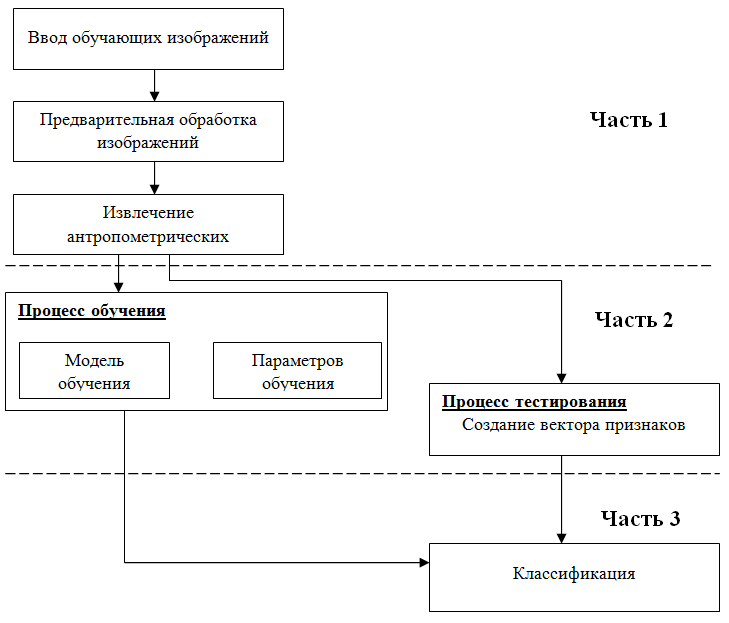
\includegraphics [scale=0.8] {images/h7.png}
\begin{center}
%\captionsetup{justification=justified, labelsep=period}
\caption{Блок-схема антропометрической системы} \label{img7}
\end{center}
\end{figure}
Система предназначена для использования в различных областях, таких как интернет-магазины для помощи пользователям в выборе размера одежды и фитнес-приложения.
%-------------------------
\section{Алгоритм извлечения антропометрических признаков из видео}

Процесс извлечения антропометрических признаков включает следующие этапы:

\begin{itemize}
	\item Предварительная обработка и нормализация изображения: на этом этапе необходимо выполнить фильтрацию шума и сглаживание изображения, применить морфологические операторы для улучшения качества контура объекта, для увеличения диапазона яркости изображений провести эквализацию их гистограмм (представлено в разделе \ref{part2.2.1});
	\item Использование алгоритма вычитания фона для обнаружения объектов: На этом шаге применяется два различных алгоритма: вычитание фона и на основе метода порогового значения. Применение для изображений и видео, полученных с камеры (представлено в разделе в \ref{part2.2.2});
	\item Использование алгоритма сегментации изображений и поиска ближайших точек границы чтобы найти местонахождение и контуры частей человеческого тела. На этом шаге применяется алгоритм разреза на графах для сегментации изображений и поиска частей человеческого тела, алгоритм обнаружения контура, итеративный алгоритм ближайших точек (Iterative Closest Point-$ICP$) для определения и корректировки точек признаков, которые ближе всего к их фактическим границам;
	\item Сравнительный анализ извлеченых признаков с реальными объектами для проверки точности методов и алгоритмов компьютерного зрения: на этом этапе будут сравниваться геометрические особенности частей человеческого тела с их настоящими частями, размеры которых были извлечены из реального тела, чтобы настроить соответствующие параметры.
\end{itemize}

В данной работе предложен метод извлечения антропометрических признаков из изображений и видео на основе алгоритмов компьютерного зрения предложенного подхода к задаче автоматического извлечения антропометрических признаков в режиме реального времени.


\subsection{Предварительная обработка изображения} \label{part2.2.1}
\subsubsection{Фильтрация изображений с помощью гауссового фильтра}
Шум является неотъемлемой частью любого устройства регистрации изображений и видео. Условно можно выделить следующие виды шума:

\begin{itemize}
	\item Шум  устройств захвата изображения;
	\item Смаз изображения, связанный с условиями регистрации, включая скорость и траекторию движения камеры;
	\item Независимый случайный шум;
	\item Отдельно отметим вмешательство наблюдения объектов.
\end{itemize}

В основе математической теории обработки изображений, включая фильтрацию, лежит понятие свертки (convolution) c определенным ядром (kernel, маска фильтра). Для того, чтобы выполнить преобразование была проведена «свертка» входного изображения с соответствующим (заранее выбранным) ядром. Со всеми пикселями в изображении проводятся свертка с ядром свертки (\ref{eq1}) (центр окна свертки будет размещен в позиции пикселя, вычисляется свертка), изменение исходных значений пикселей.
\begin{equation}\label{eq1}
Y\left(m,n\right)=X\left(m,n\right)\ast H\left(k,l\right)=\sum^r_{k=-r}\sum^r_{l=-r}X\left(m-k,n-l\right)H\left(k,l\right),
\end{equation}

\begin{itemize}
	\item $X\left(m,n\right)$ - исходная матрица размера изображения $m\ast n$;
	\item $H\left(k,l\right)$ - матрица ядра свертки, также известная как маска;
	\item $Y\left(m,n\right)$ - выходная матрица свертки между $X$ и $H$.
\end{itemize}

В данной работе использован фильтр Гаусса для удаления шума. Сущность этого преобразования состоит в реализации свертки оригинального изображения с ядром симметричной формы в виде 2-D функции Гаусса. Эта непрерывная функция определяется следующим образом:
\begin{equation}\label{eq2}
f\left(x,y\right)=\frac{1}{2\pi\sigma^2}exp\left(-\frac{x^2+y^2}{2\sigma^2}\right).
\end{equation}

Теория линейной и нелинейной фильтрации изображений является областью проведения активных научных исследований \cite{Sizikov2011,Sizikov260,Sizikov2012}.
\subsubsection{Метод бинарной морфологии}
В настоящее время методы цифровой обработки изображений привлекли внимание многих исследователей и разработчиков. Отдельно отметим метод морфологической обработки изображений.

Морфологическая обработка изображений дает количественное описание структуры и геометрии объектов в изображении, основанной на математической теории, таких как теории множеств, топологии, теории вероятности и т.д.

В приложениях компьютерного зрения морфологическая обработка используется для идентификации объектов, повышении качества изображения, сегментации изображения и проверки ошибок на изображении. Операции морфологической обработки выполняются в основном на бинарном изображении.

\textbf{Структурные элементы} \cite{Burger2009}.  В бинарном изображении, Структурный элемент представляет собой небольшое изображение, состоящий из двух значений $0$ и $1$, при этом $0$ значения игнорируются в процессе вычисления, $H\left(i,j\right)$ является структурные элементы бинарного изображения и выражается следующим образом: $H\left(i,j\right) \in \left\{0,1\right\}$.

Некоторые формы структурных элементов, обычно используемые в бинарном изображении: горизонтальные и вертикальные линии, квадраты, эллипсы и пр.

\begin{figure}[ht!]
\centering
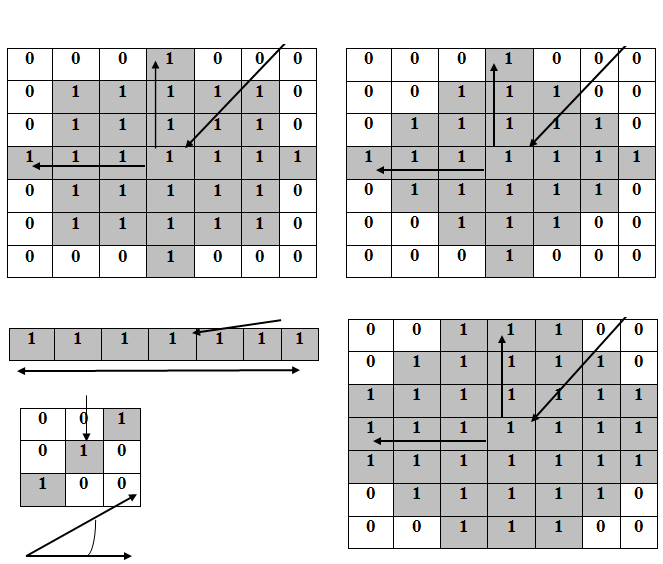
\includegraphics [scale=0.8] {images/h8.png}
\begin{center}
%\captionsetup{justification=justified, labelsep=period}
\caption{Описание формы структурных элементов.} \label{img8}
\end{center}
\end{figure}
Цель метода морфологической обработки - найти связанные компоненты контура объекта для получения идеального контура.

Операции дилатации, эрозии, открытия и закрытия могут быть применены для серого изображения. Эта концепция аналогична для бинарных морфологических операций.
\begin{equation}\label{eq3}
 g=\left(f\oplus b \right)-\left(f\ominus b\right),
\end{equation}
Где:

\begin{itemize}
	\item $f\oplus b$ является преобразованием расширения растяжением $f$ по структурным элементам b в положении $\left(x,y\right)$ по формуле:
	\begin{equation}\label{eq4}
\left[f\oplus b\right]\left(x,y\right)=max_{\left(s,t\right)\in b}\left\{f\left(x-t,y-t\right)\right\}.
\end{equation}
\item $f \ominus b$ является преобразованием эрозии растяжением $f$ по структурным элементам b в положении $\left(x,y\right)$ по формуле:
	\begin{equation}\label{eq5}
\left[f \ominus b\right]\left(x,y\right)=max_{\left(s,t\right)\in b}\left\{f\left(x+t,y+t\right)\right\}.
\end{equation}
\end{itemize}
Набор пикселей, которые соединяются с другими называется компонентой связности \cite{Solomon2011}. Пиксели соединены друг с другом, которые отличаются от других групп пикселей назначенной им меткой. Эти метки представляют собой целые числа, где фон имеет значение $0$, область изображения $/$ группа взаимосвязанных пикселя помечена $1$.
\begin{figure}[ht!]
\centering
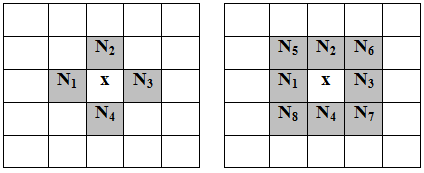
\includegraphics [scale=0.8] {images/h9.png}
\begin{center}
%\captionsetup{justification=justified, labelsep=period}
\caption{Форма 4 соседей (N4) и 8 соседей (N8).} \label{img9}
\end{center}
\end{figure}
В данной работе используются алгоритмы для обозначения 8-связных компонент (рис.\ref{img9}). Алгоритм включает в себя следующие этапы:

\begin{itemize}
	\item Шаг 1: Сканирование входных изображений последовательно по строкам сверху-внизу, чтобы встретить любую точку $p$ $\left(p=1,если бинарное изображен\right)$ в изображении;
	\item Шаг 2: Проверка соседей $p$. На основе этой информации, метка будет осуществляться следующим образом:
	
	\begin{itemize}
		\item Если все соседи со значением равным нулю, то $p$ присваивается новая, ранее не использовавшаяся метка.
		\item Если имеется только один соседний пиксел $р$ со значением $1$, присваиваем эту метку пикселу $р$;
		\item Если имеется больше чем один соседний пиксел $р$ со значением $1$, присваиваем метку любого из уже пронумерованных пикселов.
	\end{itemize}
	
\end{itemize}
После завершения процесса сканирования, соответствующие пары метки располагаются в соответствующие группы, и каждой группе будет присвоена только одна метка.
\subsubsection{Метод выравнивания гистограммы}
При регистрации изображений и видео при помощи всегда происходит дисбаланса света. Эта проблема может быть легко решена путем воздействия на источник света в случае лабораторных условиях регистрации.

Настоящая работа направлена на создание практических приложений для смартфонов, которые могут работать в реальных условиях освещения. Таким образом, автоматический баланс яркости является необходимым требованием для разрабатываемого комплекса программ. Используется метод эквализации гистограммы для решения задачи.

Эквализация гистограммы является простой теорией и часто используется при обработке изображений. Цель эквализации гистограммы, как уже отмечалось выше, заключается в увеличении диапазона яркости изображения.

Эквализация гистограммы изображения g определяется следующим образом:
\begin{equation}\label{eq6}
g_{i,j}=floor\left(\left(L-1\right)\sum^{f_{i,j}}_{n=0}p_n\right),
\end{equation}
Где:

\begin{itemize}
	\item $f$ - исходное изображение;
	\item $n=0,1,…,L-1;L \in \left[0 ; 255\right]$;
	\item $p_n$:Количество пикселей по интенсивности  n / Количество пикселей;
	\item $floor()$ округляется до ближайшего целого числа. Это эквивалентно преобразованию интенсивности пикселей, $k$, $f$ с помощью функции:
	\begin{equation}\label{eq7}
T\left(K\right)=floor\left(\left(L-1\right)\sum^k_{n=0}p_n\right).
\end{equation}
\end{itemize}
Этот метод имеет преимущество простоты, легкости применения, без каких-либо серьезных расчетов, он используется в случаях, когда необходимо привести изображение в его <<нормальное>> состояние.

%-------------------------
\subsection{Алгоритмы вычитания фона изображения для обнаружения объектов в видео} \label{part2.2.2}
Вычитание фона является одним из наиболее популярных используемых алгоритмов в области компьютерного зрения. Алгоритм используется для определения пикселей движущихся объектов в видео, также известных как передний план (FG - foreground), в то время как неподвижный объект называется фоном (BG - background). Алгоритм вычитания фона используется на этапе предварительной обработки в многих задачах компьютерного зрения, результаты этого шага могут существенно повлиять на исход следующих шагов (идентификация, отслеживание, и т.д.).

В данной работе представлены решения для задачи вычитания фона, такие как построение модели на основе гауссовой смешанной модели.

Эта модель используется чтобы обнаружить движущиеся объекты в текущем кадре. Проведено много исследований по методу построения моделирования фона, например в \cite{Mittal2004} авторы использовали адаптивную плотность оценки (adaptive kernel density estimation) и получили хорошие результаты, однако, существует недостатки: требуется большой объем дискового пространства, вычислительная сложность, скорость работы не соответствует реальному времени. В работе \cite{Stauffer2009} Стауффер использовал гауссову смесь (Mixture of Gaussian) в построении модели фона для обнаружения движения. 

Основная идея алгоритма вычитания фона следующая. Пиксель в положении $x$ в изображении принадлежит объекту, если она удовлетворяет неравенству:

	\begin{equation}\label{eq8}
\left|I_n\left(x\right)-B_n\left(x\right)\right| \geq T_n\left(x\right),
\end{equation}

Где:

\begin{itemize}
	\item $I_n\left(x\right) \in \left[0,255\right]$  - значение интенсивности серого в позиции пикселя $x$ принадлежит $n$-му изображению или видеофрагменту;
	\item $B_n \left(x\right)$  - значение интенсивности фона в местоположении пикселя $x$;
	\item $T_n \left(x\right)$  - пороговое значение задается для каждого изображения. 
\end{itemize}
Модель базового фона постоянно обновляется из исходных изображений или видео. На месте расположения пикселей на изображении, разные кадры будут давать разные значения. Например, значение пикселя в позиции х на изображении фона отличается от значения пикселя в позиции х на изображении переднего плана.
\begin{equation}\label{eq9}
B_{n+1}\left(x\right)= \left\{\begin{array}{l} \alpha B_n\left(x\right)+\left(1-\alpha\right)I_n\left(x\right),x\in BG,\\
\beta B_n\left(x\right)+\left(1-\beta\right)I_n\left(x\right),x\in FG,
\end{array}\right.
\end{equation}
где BG - соответствует фону, а FG - переднему плану. Пороговое значение пикселя в позиции $x$ является:
\begin{equation}\label{eq10}
T_{n+1}\left(x\right)= \left\{\begin{array}{l} \alpha T_n \left(x\right)+\left(1-\alpha\right) \left(\left|I_n\left(x\right)-B_n\left(x\right)\right|\right), x \in BG,\\
T_n\left(x\right), x\in FG,
\end{array}\right.
\end{equation}

Параметры $\alpha$, $\beta$ выбираются из интервала $\left[0,1\right]$ для обеспечения обновления фона в изображении и видео. Блок схема алгоритма вычитания фона на основе пороговых значений представлена на (рис. \ref{img10}), а алгоритм обновления фона - на (рис. \ref{img11}).

\begin{figure}[ht!]
\centering
\begin{center}
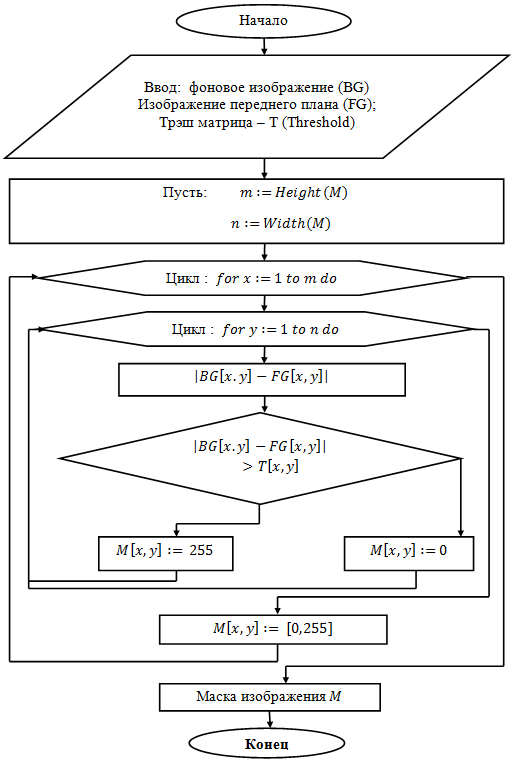
\includegraphics [scale=1] {images/h10.png}
%\captionsetup{justification=justified, labelsep=period}
\caption{Блок-схема алгоритма вычитания фона.} \label{img10}
\end{center}
\end{figure}

\begin{figure}[ht!]
\centering
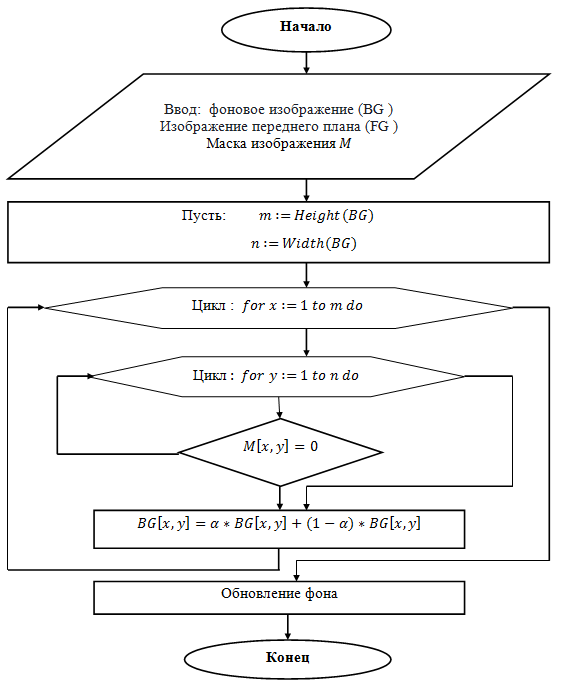
\includegraphics [scale=1] {images/h11.png}
\begin{center}
%\captionsetup{justification=justified, labelsep=period}
\caption{Блок-схема алгоритма обновления фона.} \label{img11}
\end{center}
\end{figure}

Каждый пиксель моделируется как случайный вектор. Значение пикселя $x$ в момент времени $t : x^{\left(t\right)}$. Значения пикселей на основе распределения гауссово смеси:

\begin{equation}\label{eq11}
P\left(0|\theta\right)=\sum^K_{k=1}\pi_kN\left(x|\mu_k,\beta_k\right).
\end{equation}

Для обновления фона в видео, модель фона должна постоянно обновляться, с помощью случайной выборки $X=\left\{x^{\left(t\right)},..., x^{\left(t-T\right)}\right\}$для оценки параметров модели. Метод максимального распределения (Maximize Posteriori) используется для оценки подходящих параметров в гауссовой модели по формуле:
\begin{equation}\label{eq12}
\hat{\theta} = argmax_\theta \left\{\ln p\left(X|\theta\left(K\right)\right)+\ln p\left(\theta\left(K\right)\right)\right\},
\end{equation}
Где:

\begin{itemize}
	\item $K$ параметр модели;
	\item $P\left(\theta\left(K\right)\right)$Функция распределения параметра $\pi\left(K\right)\equiv\left\{\pi_1, ..., \pi_K\right\}$.
\end{itemize}

Согласно \cite{Bishop2006}
\begin{equation}\label{eq13}
\frac{\partial}{\partial\theta}\left\{\ln P\left(X|\theta\left(K\right)\right)+\ln P\left(\theta\left(K\right)\right)+\gamma\left(\sum^K_{k=1}\pi_k-1\right)\right\},
\end{equation}
\begin{equation}\label{eq14}
\longleftrightarrow \frac{\partial}{\partial\theta}\left\{\sum^t_{n=1}ln\left\{\sum^N_{k=1}\pi_kN\left(x^{\left(n\right)}|\mu_k,\beta_k\right)\right\}-\frac{c}{2}\sum^N_{k=1}ln \pi_k + \gamma\left(\sum^K_{k=1}\pi_k-1\right\}\right) = 0,
\end{equation}
Где:
 $c=\frac{N}{2}$, $N$ - каличество параметров для каждой модели компонента \cite{Figueiredo2002}.
\begin{equation}\label{eq15}
\hat{\pi}^{\left(t\right)}_k = \frac{\hat{\pi}^{\left(t\right)}_k\frac{c}{t}}{1-K\frac{c}{t}},
\end{equation}
\begin{equation}\label{eq16}
\mu^{\left(t\right)}_k = \frac{1}{N_k}\sum^t_{n=1}\gamma^{\left(t\right)}\left(z^{\left(n\right)}_k\right)x^{\left(n\right)},
\end{equation}
\begin{equation}\label{eq17}
\beta^{\left(t\right)}_k =\frac{1}{N_k}\sum^t_{n=1}\gamma^{\left(t\right)}\left(z^{\left(n\right)}_k\right)\left(x^{\left(n\right)}-\mu^{\left(n\right)}_k\right)\left(x^{\left(n\right)}-\mu^{\left(n\right)}_k\right)^T.
\end{equation}
Для построения алгоритма обновления фона, необходимо использовать наблюдаемое значение и поэтому предыдущий результат построения обновляется. Уравнение обновления модели описывается следующим образом:
\begin{equation}\label{eq18}
\hat{\pi}^{\left(t+1\right)}_k=\hat{\pi}^{\left(t\right)}_k + \left(t-1\right)^{-1} \left(\frac{\gamma z^{\left(t\right)}_k}{1-K\frac{c}{T}} - \hat{\pi}^{\left(t\right)}_k\right) - \left(1-t\right)^{-1} \frac{\frac{c}{T}}{1-K\frac{c}{T}},
\end{equation}
\begin{equation}\label{eq19}
\hat{\mu}^{\left(t+1\right)}_k = \hat{\mu}^{\left(t\right)}_k + \left(t+1\right)^{-1} \frac{\gamma^{\left(t\right)}z^{\left(t+1\right)}_k}{\hat{\pi}^{\left(t\right)}_k}\left(x^{\left(t+1\right)}-\hat{\mu}^{\left(t\right)}_k\right),
\end{equation}
\begin{equation}\label{eq20}
\hat{\beta}^{\left(t+1\right)}_k = \hat{\beta}^{\left(t\right)}_k + \left(t+1\right)^{-1} \frac{\gamma^{\left(t\right)}z^{\left(t+1\right)}_k}{\hat{\pi}^{\left(t\right)}_k} \left(x^{\left(t+1\right)}-\hat{\mu}^{\left(t\right)}_k\right)\left(x^{\left(t+1\right)}-\hat{\mu}^{\left(t\right)}_k\right)^T - \hat{\beta}^{\left(t\right)}_k.
\end{equation}

Уравнение (\ref{eq18}) строится из (\ref{eq15}) с $\frac{c}{t}=\frac{c}{T}$  с применением гауссовой модели, чтобы обновить модели фона, помочь алгоритму вычитания фона работать быстрее в режиме реального времени и хорошей точности.



%-------------------------
\subsection{Сегментация изображений при помощи разрезов на графах}
Сегментация изображений является одним из важных шагов в процессе компьютерного зрения. Сегментация изображений играет большую роль в анализе изображений и в получении важной информации из изображений.

На практике сегментация изображений имеет две сложные проблемы: слабые границы и структуры. Первая проблема состоит в нахождении слабых границ, когда они являются частью соответствующей границы. Вторая проблемма заключается в разделении сложных структур в изображении \cite{Sagiv2006, Raviv2007}. На самом деле, такие ситуации часто возникают в практике. В этом случае сегментация становится неясной без добавления априорной информации пользователей. Поэтому, использование методов сегментации изображений с учителем широко используется.

В настоящее время существует много алгоритмов предлагаемых для решения задач сегментации изображений. Существует три типа алгоритмов сегментации обучения с учителем, основанных на исходной информации от пользователей:

\begin{itemize}
	\item Первый тип является результатом сегментации на основании желательных границ, например Intelligent Scissors \cite{Mortensen1995};
	\item Второй тип является  результатом сегментации на основании исходных границ, которые находятся близко с желательными границами, например Active Contour \cite{Lankton} и Set Level \cite{Lie2006};
	\item Третий тип является результатом сегментации на основании маркировки пикселей, которые задаются пользователами.
\end{itemize}
Одним из популярных подходов является метод разреза на графах, которые основаны на функции энергии. В этом методе изображение представляется как взвешенный неориентированный граф. Обычно пиксель или группа пикселей ассоциируется вершиной, а веса рёбер определяют (не)похожесть соседних пикселей. Затем граф (изображение) разрезается согласно критерию, созданному для получения «хороших» кластеров. Каждая часть вершин (пикселей), получаемая этими алгоритмами, считается объектом на изображении.

\textbf{Проблема о максимальном потоке} (maximum flow problem): найти поток $f$ такой, что величина потока максимальна. 
\[
f: \sum_u f\left(u\rightarrow v\right)=\sum_wf\left(v\rightarrow w\right). 
\]

Величина потока (value of flow) — сумма потоков из источника.
\[
\left|f\right|:= \sum_w f \left(s\rightarrow w\right) - \sum_u f\left(u\rightarrow s\right).
\]

\textbf{Минимальный разрез} — разрез с минимальной пропускной способностью. 
$C_{min} \left(A,B\right)=\sum_{u\in S, v \in T} W_{uv}$.

Разрез (s-t cut) — разбиение множества всех вершин V на два подмножества $A$ и $B$ таких, что $s\in A $, $t\in B$, причем пересечение $A$ и $B$ равно пустому множеству. Если рассматривать весовые коэффициенты, связанные с каждым узлом в качестве емкости потока, можно показать, что максимальное количество энергии потока от источника равно емкости минимального разреза. Поэтому проблема минимального разреза также известна как проблема максимального потока. Нужно выбрать необходимый поток и необходимый разрез $\left(S, T\right)$, а затем следить неравенством \cite{Boykov12001}:
\begin{equation}\label{eq21}
\left|f\right| = \sum_w f\left(s\rightarrow w\right) - \sum_u f \left(u\rightarrow s\right),
\end{equation}
\[
=\sum_{v\in S}\left(\sum_w f \left(v \rightarrow w \right) - \sum_u f\left( u \rightarrow v \right) \right),
\]
\[
= \sum_{v \in S} \left(\sum_{w \in T} f \left( v \rightarrow w\right) - \sum_{u \in T} f \left( u \rightarrow v \right)\right),
\]
\[
\leq \sum_{v \in S}\sum_{w \in T} f \left( v \rightarrow w \right) после  f \left(u \rightarrow v\right) \geq 0,
\]
\[
\leq \sum_{v \in S}\sum_{w \in T} c \left(v\rightarrow w \right)  после f \left(u \rightarrow v \right) \leq c \left( v \rightarrow w\right),
\]
\[
=\left\|S, T\right\|.
\]

Грань между пиксельной $i$ и $j$ будем обозначать $W^I_{ij}$ и терминал весов между пиксельной $i$ и источником $\left(s\right)$ и мойкой $\left(t\right)$. $W^s_i$ и $W^t_i$ соответственно задаются \cite{Parvathy}:
\begin{equation}\label{eq22}
W^i_{ij} = e^{\left(-\frac{r\left(i,j\right)}{\sigma R}\right)}e^{\left(-\frac{\left\|w\left(i\right)-w\left(j\right)\right\|^2}{\sigma W}\right)},
\end{equation}
\begin{equation}\label{eq23}
W^s_i = \frac{p\left(w\left(i\right)| i \in s\right)}{p \left(w \left(i\right)\right)|i \in s + p \left(w\left(i\right)|i \in t\right)},
\end{equation}
\begin{equation}\label{eq24}
W^t_i = \frac{p\left(w\left(i\right) | i \in t\right)}{p \left(w \left(i\right)\right)|i \in s + p \left(w\left(i\right)|i \in t\right)}.
\end{equation}
Где:

\begin{itemize}
	\item $r\left(i,j\right)$ расстояние между пиксельной $i$ и $j$;
	\item $\left\|.\right\|$ обозначает евклидову норму;
	\item $\sigma R$ и $\sigma W$ настраивают параметры, взвешивая различные значения;
	\item $W^I_{ij}$ содержит сходство между пикселями;
	\item $W^s_i$, $W^t_i$ описывает пиксель фона и переднего плана соответственно.
\end{itemize}
В сегментации изображений обычно имеется задача разбиения на $2$ области : объект foreground и фон. Данный метод стал основой большинства современных наилучших методов интерактивной сегментации, так что остановимся на этом алгоритме подробнее.

На входе данный алгоритм разреза графов получает исходные данные изображений и добавление информаций от пользователей: количество пикселей объекта, области вокруг объекта, приблизительную границу объекта \cite{Boykov2001}. Чтобы ограничить ошибки в сегментации изображения для решения требований практических задачи, пользователь обеспечит необходимые данные каждому случаю. Дан граф $G\left(V,E\right)$ с пропускной способностью $c\left(u,v\right)$ и потоком $f\left(u,v\right)=0$ для ребер из $u$ в $v$. Необходимо найти максимальный поток (Max – flow) из источника $s$  (source) в сток $t$ (sink). На каждом шаге алгоритма действуют те же условия, что и для всех потоков \cite{Cormen2001}:

\begin{itemize}
	\item $f\left(u,v\right) \leq c\left(u,v\right)$ - Это поток из u в v не превосходит пропускной способности;
	\item $f\left(u,v\right) =-f\left(v,u\right)$;
	\item $\sum_vf\left(u,v\right)=0 \leftrightarrow f_{in}\left(u\right) =f_{out}\left(v\right)$ для всех узлов $u$, кроме $s$ и $t$;
	\item Остаточная сеть $G_f\left(V,E_f\right)$ - сеть с  пропускной способностью $c_f\left(u,v\right)=c\left(u,v\right)-f\left(u,v\right)$ и без потока Ford – Fulkerson (1956) \cite{Ford1956}. Максимальный поток на основе алгоритма (\ref{img12}).
\end{itemize}

\begin{figure}[ht!]
\centering
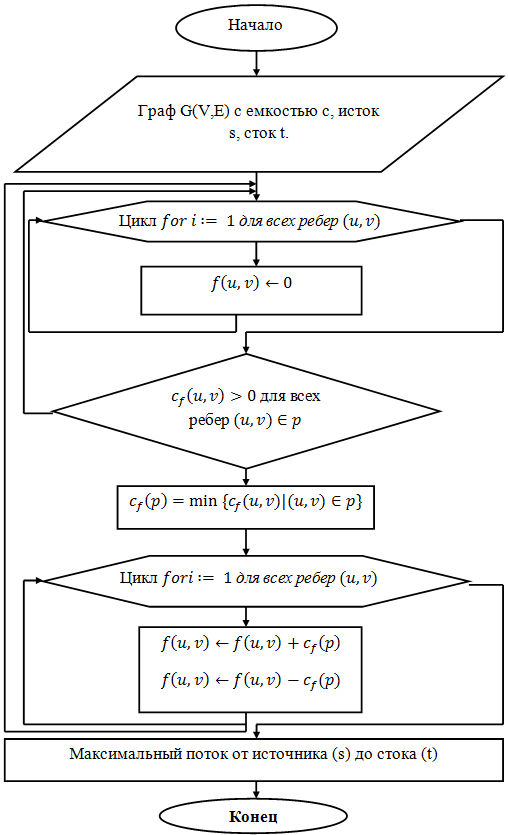
\includegraphics [scale=1] {images/h12.png}
\begin{center}
%\captionsetup{justification=justified, labelsep=period}
\caption{Блок-схема алгоритма разреза на графах.} \label{img12}
\end{center}
\end{figure}

Метод разреза графов находит сильные локальные минимумы энергетической функции. Метод достаточно мощный, чтобы решать множество полезных задач, и он может быть применен к решению проблемы графика min-среза. 
\begin{equation}\label{eq25}
E\left(f\right) = \sum_{p \in P}D_p\left(f_p\right)+\sum_{p,q \in N}V_{p,q}\left(f_p,f_q\right).
\end{equation}
Найти маркировки $f:P\rightarrow L$ , что сводит к минимуму $E\left(f\right)$ из множеств пикселей $P$, набор этикеток $L,N \in P$ является система соседства по пикселям. $D_p\left(f_p\right)$ является функцией, которая получена из данных наблюдений, и которая измеряет стоимость присвоения метки $f_p$ на пиксель $p$. $V_{\left(p,q\right)} \left(f_p,f_q\right)$ , и измеряет стоимость присвоения метки $f_p$,$f_q$ на соседние пиксели $p$, $q$. Используется для улучшения пространственного сглаживания \cite{Boykovv2001, Boykov2004}.

На каждом шаге алгоритм выполняет каждый поток, который соединяет от $s$ к $t$. Сложность алгоритма зависит от числа ребер, осуществляется по индукции всех потоков. Движение потока увеличивается, по меньшей мере один раз на каждом шаге алгоритма. Поэтому, сложность алгоритма не превосходит $O\left(f\right)$, где  $f$ - максимальный поток в графе.  $E$ - это число ребер графа, так что сложность будет $О\left(E\ast f\right)$.

После этого в полученном графе находится минимальный разрез, который делит граф на $2$ части. Вес ребер между метками обеспечивает выполнение заданных пользователем ограничений: маркировки объекта будут отнесены к объекту, маркировки фона - к фону.

%-------------------------
\subsection{Итеративный алгоритм ближайших точек}
Итеративный алгоритм ближайших точек Paul J. Besl и Neil D. Mackay представили в научном журнале IEEE впервые в феврале 1992 года \cite{Besl1992}. Итеративный алгоритм ближайших точек  используется для минимизации расстояния между двумя заданными точками. Алгоритм широко используется в построения на основе изображения 3D \cite{Gelfan2003, Rusinkiewicz2001}. Для сокращения времени вычислений и улучшить сходимость итерационных ближайшей точки (ICP) в ключевых точках экстракции. В каждой итерации $ICP$, то RANSAC \cite{Hast2013} вкладывается, чтобы удалить выбросы и сходимость $ICP$ гарантируется.  Алгоритм $RANSAC$ часто используется в компьютерном зрении. Преимуществом алгоритма $RANSAC$ является его способность дать надёжную оценку параметров модели, то есть возможность оценить параметры модели с высокой точностью, даже если в исходном наборе данных присутствует значительное количество выбросов.
В данной работе алгоритм $ICP$ используется чтобы уменьшить отклонение конкретных точек на контуре человеческой части. Созданный набор признаков используется для сравнения с множеством точек, извлечённых с объекта. Для простого сравнения потребуется время и ресурсы системы. Результаты получаются не такие, как ожидались. Форма движения и шум будут влиять на результаты работы программы. Таким образом, чтобы преодолеть эту проблему используется алгоритм $ICP$, чтобы уменьшить различия между этими двумя наборами точек.

Полученным результатом является набор признаков объекта, находящегося близко к контуру 2D тела человека на фотографии. Мы провели уточнения контура пикселей на объекте с помощью алгоритма $ICP$ (рис \ref{img13}).
\begin{figure}[ht!]
\centering
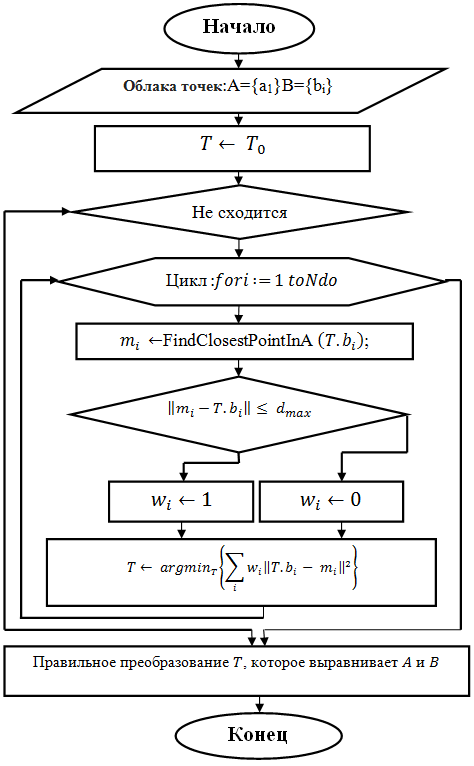
\includegraphics [scale=1] {images/h13.png}
\begin{center}
%\captionsetup{justification=justified, labelsep=period}
\caption{Блок-схема алгоритма $ICP$} \label{img13}
\end{center}
\end{figure}
В набор точек признаков, найденных на объекте, $29$ точек имеют признаки, извлеченные с атрибутами характерной геометрии: выпуклые, вогнутые кривые, соответствующие важным позициям, связанными с измерением размеров частей тела. Алгоритм включает в себя основные шаги:

\begin{itemize}
	\item \textbf{Шаг 1:} Вычислим соответствия между двумя сканированиями;
	\item \textbf{Шаг 2:} Выполним преобразование, которое сводит к минимуму расстояние между соответствующими точками.
\end{itemize}
Используем соответствующее максимальное пороговое значение $d_{max}$. Здесь $d_{max}$ представляет собой баланс между сходимостью и точностью.

Алгоритм $ICP$ повторяет действия, чтобы минимизировать среднеквадратичную ошибку пикселов, соответствующих ближайшей точке.
\begin{equation}\label{eq26}
T\leftarrow argmin_t\left\{\sum_i\left\|T.b_i - m_i\right\|^2\right\}.
\end{equation}
Где:

\begin{itemize}
	\item $T$ - правильное преобразование;
	\item $b_i$: $B=\left\{b_i\right\}$ - Облака точек;
	\item $m_i$ - множество точек, которые будут преобразованы из $B$ - $A$ ( $A=\left\{a_i\right\}$ - Облака точек);
\end{itemize}

Набор новых точек будет найден, если он удовлетворяет двум условиям:

\begin{itemize}
	\item Расположен на границе или наиболее близко к границам объекта;
	\item Расстояние между двумя наборами точек является наименьшим.
\end{itemize}
Таким образом, получен набор новых признаков для описания точного контура объекта.

Этапы алгоритма ICP выполнются последовательно. Алгоритм остановится только, если имеет место сходимость (наименьшая ошибка и стабильность). Алгоритм $ICP$ с такими операциями всегда монотонно сходится на интервале области определения функции. Тем не менее параметры алгоритма зависят от настройки. Таким образом, алгоритм $ICP$ будет сходиться на всей области определения функции. В то же время, новые точки признаков абсолютно совпадают с точками признаков в базе данных.
%-------------------------
\subsection{Извлечение антропометрических признаков из видео}
Для решения задачи извлечения антропометрических признаков с изображения и видео предложен алгоритм, основанный на  комбинации новейших методов - технике предварительной обработки изображений, алгоритме вычитания фона, алгоритме сегментации изображений на основе разреза графов, алгоритме итеративных ближайших точек.

Процесс извлечения антропометрических признаков объектов на изображении и видео на основе алгоритма компьютерного зрения включает в себя следующие этапы (рис \ref{img14}):
\begin{itemize}
	\item \textbf{Шаг 1:} Предварительная обработка изображения;
	
	\begin{itemize}
		\item Фильтр шума с гауссовым фильтром с матрицей фильтра окна $\left[5 5\right]$;
		\item Используем морфологические операторы - дилатации, чтобы улучшить качество точек изображения со структурами элементов $se=strel\left(line,11,90\right)$;
		\item Эквализация гистограммы.
	\end{itemize}
	\item \textbf{Шаг 2:} Обнаружение объекта и человеческого лица. Важную роль на этом шаге играет алгоритм вычитания фона. Расчетные значения пикселей на разных кадрах получаем по формуле (\ref{eq9});
	
	Метод Виола-Джонса \cite{Violaj2001, Viola2004} используется для обнаружения человеческого лица с изображения. Метод состоит из трех основных этапов: интегральном представлении изображения, метод построения классификатора на основе алгоритма адаптивного бустинга (AdaBoost) и метод комбинирования классификаторов в каскадную структуру.
	\item \textbf{Шаг 3:} Сегментация изображения методом разреза на графах. Поиск области изображения, содержащего части тела человека на основе формулы (\ref{eq25});
	\item \textbf{Шаг 4:} Обнаружение контура и поиск ключевых точек признаков – алгоритм $ICP$. Расчет евклидова расстояния: $d\left(A,B\right) = \sqrt{\left(x_B - x_A\right)^2 + \left(y_B - y_A\right)^2}$;
	\item \textbf{Шаг 5:} Создание антропометрического вектора признаков.
\end{itemize}

\begin{figure}[ht!]
\centering
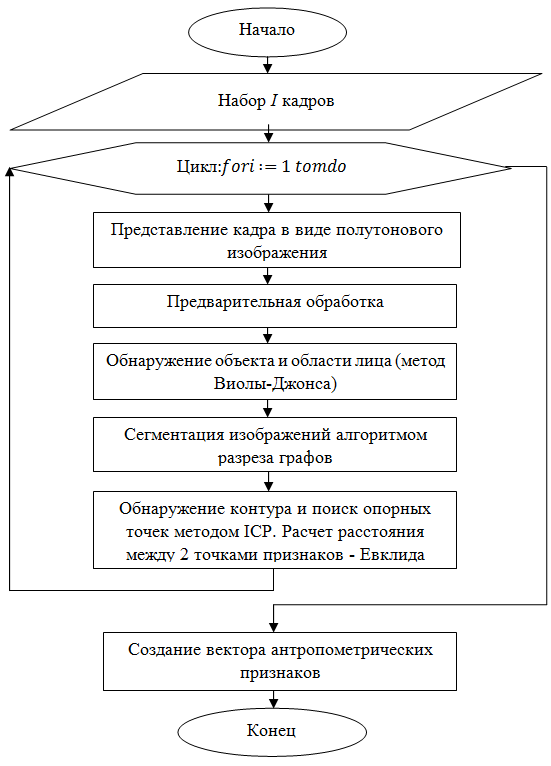
\includegraphics [scale=1.05] {images/h14.png}
\begin{center}
%\captionsetup{justification=justified, labelsep=period}
\caption{Блок-схема алгоритма извлечения антропометрических признаков из видеопоследовательности.} \label{img14}
\end{center}
\end{figure}
%-------------------------
%-------------------------
\section{Оценивание точности метода извлечения антропометрических признаков}
В этой части представлен результат извлечения антропометрических признаков на основе алгоритма компьютерного зрения из $50$ изображений. Извлечение ключевых точек (меток - опорных точек) состоит из $2$ главных этапов:

\begin{itemize}
	\item \textbf{Шаг 1:} Предварительная обработка изображения, преобразование исходного цветного изображения в изображение в оттенках серого, фильтрация шумов, разряжение пикселей, эквализация гистограммы для получения лучшего качества изображения;
	\item \textbf{Шаг 2: } Извлечение точек признаков с использованием алгоритма вычитания фона, обнаружения человеческого лица, сегментации изображения, поиска опорных точек для вычисления антророметрических признаков.
\end{itemize}

Для оценки эффективности процесса извлечения признаков применяются средняя абсолютная ошибка - $MAPE$:
\begin{equation}\label{eq26}
M=\frac{1}{n}\sum^n_{i=1}\left|\frac{A_t-F_t}{A_t}\right|,
\end{equation}
Где:

\begin{itemize}
	\item $A_t$: Результат измерений, рассчитанных вручную;
	\item $F_t$: Результат извлечения антропометрических признаков.
\end{itemize}
Эксперимент был использован для проверки погрешности размеров человеческих частей на основе извлечения количества признаков. На основании результатов для калибровки точности алгоритма.

\textbf{Случай 1}: Результат извлечения 24 опорных точек на контуре человеческого тела. Иллюстрация расположения опорных точек (рис. \ref{img15}): 
\begin{figure}[ht!]
\centering
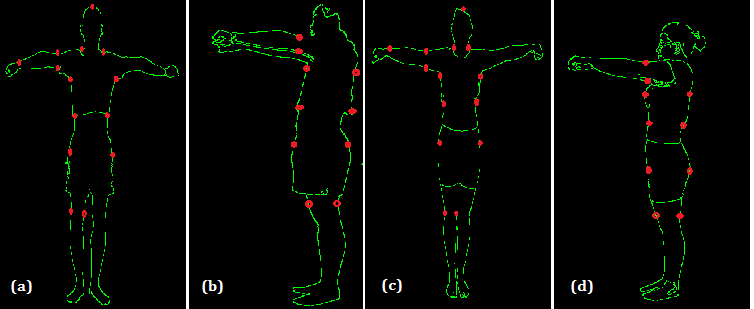
\includegraphics [scale=0.8] {images/h15.png}
\begin{center}
%\captionsetup{justification=justified, labelsep=period}
\caption{Результат расположения 24 опорных точек \cite{long1,long2}.} \label{img15}
\end{center}
\end{figure}

\begin{table}[b!]%
\begin{center}
\caption{Результат извлечения антропометрических признаков и погрешности системы компьютерного зрения \cite{long1,long2}.}\label{tab1}
  \begin{tabular}{|c|c|c|c|c|c|c|}
    \hline
    \multirow{2}{*}{Антропометрические} & {Ручной} & \multicolumn{3}{c}{Результаты системы} & {$\sum^n_{i=1}\left|\frac{A_t-F_t}{A_t}\right|$} &{$M$} \\
      признаки& метод &1 &2 &3& & \\
    \hline
Груди &95	&93.65	&94.11	&93.32	&0.04126	&0.01375\\
\hline
Талия               &79	&76.06	&78.80	&80.15	&0.05430	&0.01810\\
\hline
Бедра               &96.5	&93.07	&95.19	&95.78	&0.05658	&0.01886\\
\hline
Длина рук           &53	  &52.45	&54.32	&54.72	&0.06774	&0.02258\\
\hline
Обхват бицепса      &28	 &25.68	  &27.09	&27.60	&0.12964	&0.04321\\
\hline
Обхват шеи          &37	 &35.71	  &36.67	&36.79	&0.04946	&0.01649\\
\hline
Длина спины         &40	 &38.50	  &40.11	&40.01	&0.04050	&0.01350\\
\hline
Длина плеча       &36	 &35.86	  &36.19	&35.50	&0.02306	&0.00769\\
\hline
Ширина плеча         &14	 &13.91	  &13.56	&14.74	&0.09071	&0.03024\\
\hline
Высота груди        &18	 &17.78	  &17.60	&17.86	&0.04222	&0.01407\\
\hline
  \end{tabular}
\end{center}
\end{table}%\vspace{10mm}

\textbf{Случай 2:} Применение метода калибровки для улучшения точности извлечения признаков (рис. \ref{img152}).
\begin{figure}[ht!]
\centering
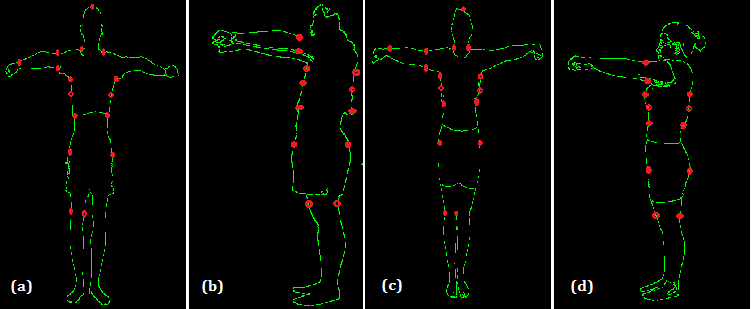
\includegraphics [scale=0.8] {images/h152.png}
\begin{center}
%\captionsetup{justification=justified, labelsep=period}
\caption{Результат расположения 28 опорных точек  \cite{long1,long2}.} \label{img152}
\end{center}
\end{figure}
\begin{table}[b!]%
\begin{center}
\caption{Результат извлечения антропометрических признаков и погрешности системы компьютерного зрения после применения калибровки извлеченных точек \cite{long1,long2}.}.\label{tab3}
  \begin{tabular}{|c|c|c|c|c|c|c|}
    \hline
    \multirow{2}{*}{Антропометрические} & {Ручной} & \multicolumn{3}{c}{Результаты системы} & {$\sum^n_{i=1}\left|\frac{A_t-F_t}{A_t}\right|$} &{$M$} \\
      признаки& метод  &1 &2 &3 & & \\
    \hline
Груди &95	&95.03	&95.00	&95.02	&0.00053	&0.00018 \\
\hline 
Талия             &79	&78.46	&79.05	&78.89	&0.00557	&0.00186\\

\hline
Бедра               &96.5	&97.29	&96.11	&96.4	&0.00010	&0.00003\\

\hline
Длина рук           &53	&52.93		&52.1	&52.93	&0.03531	&0.01177\\

\hline
Обхват бицепса      &28	&28.24	&28.03	&28.07	&0.01071	&0.00357\\

\hline
Обхват шеи         &37	&38.35	&38.13	&38.05	&0.09672	&0.03224\\

\hline
Длина спины         &40	&38.35	&39.96	&39.81	&0.04325	&0.01442\\

\hline
Длина плеча       &36	&36.01	&36.17	&36.1	&0.00971	&0.00324\\

\hline
Ширина плеча        &14	&13.97	&14.02	&14.02	&0.00071	&0.00024\\

\hline
Высота груди       &18	&18.05	&18.11	&18.01	&0.01500	&0.00500\\

\hline
  \end{tabular}
\end{center}
\end{table}%\vspace{10mm}

\begin{figure}[ht!]
\centering
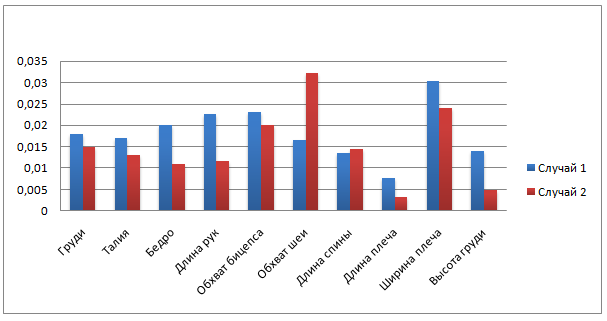
\includegraphics [scale=0.7] {images/h16.png}
\begin{center}
%\captionsetup{justification=justified, labelsep=period}
\caption{Погрешность в обоих случаях в извлечении антропометрических признаков.} \label{img16}
\end{center}
\end{figure}

\begin{figure}[ht!]
\centering
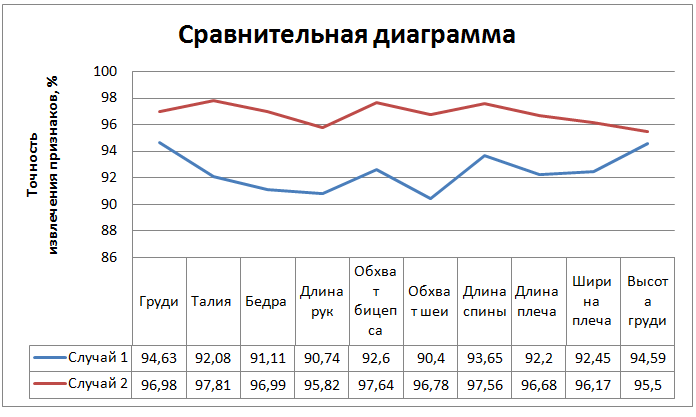
\includegraphics [scale=0.7] {images/h18.png}
\begin{center}
%\captionsetup{justification=justified, labelsep=period}
\caption{Процент правильной классификации (\%)  в обоих случаях в извлечении антропометрических признаков.} \label{img18}
\end{center}
\end{figure}

Для вычичления технической погрешности измерений при извлечении антропометрических признаков используется метод $TEM$(technical error of measurement)\cite{Stanley1999}. В данной работе выполняется извлечение антропометрических признаков 100 раз для одного человека.

С помощью метода $TEM$:

	\begin{equation}\label{eq50}
TEM=\sqrt{\left(\left(\sum_1^N\left(\left(\sum_1^K M^2\right)-\left(\left(\sum_1^K M\right)^2\right)\right)\right)/N\left(K-1\right)\right)}
\end{equation}
Где

\begin{itemize}
	\item $N$ - количество объектов;
	\item $K$ - количество выполнения;
	\item $M$ - измерение.
\end{itemize}

Получена гистограмма технической погрешности измерений (рис. \ref{img45}).

\begin{figure}[ht!]
\centering
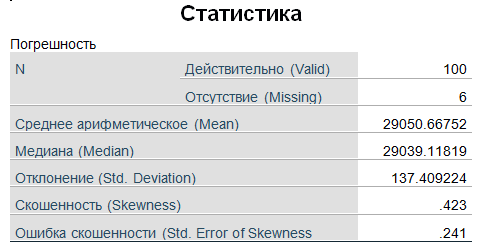
\includegraphics [scale=1] {images/h45.png}
\begin{center}
%\captionsetup{justification=justified, labelsep=period}
\caption{Результат анализа погрешности.} \label{img45}
\end{center}
\end{figure}

В (рис. \ref{img45}) показано, что среднее арифметичесное $mean = 29050.66752$, медиана $median = 29039.11819$ и скошенность $skewness= 0.423$. В этом распределении среднее арифметичесное и медиана приблизительны, скошенность $\in \left[-1;1\right]$. Поэтому это нормальное распределение (распределение Гаусса) (рис. \ref{img44}).

\begin{figure}[ht!]
\centering
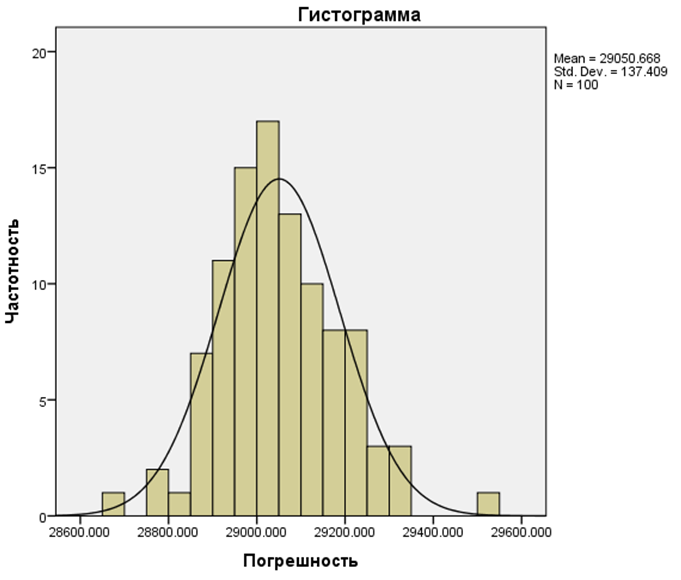
\includegraphics [scale=1] {images/h44.png}
\begin{center}
%\captionsetup{justification=justified, labelsep=period}
\caption{Гистограмма технической погрешности измерений.} \label{img44}
\end{center}
\end{figure}



  
%-------------------------
\section{Приложение алгоритма случайного леса для классификации антропометрических данных}
\subsection{Предложенная модель} В работе используется модель Wrapper \cite{Vladimir2000} с целевой функцией для оценки алгоритма случайного леса, показанная на рисунке (рис. \ref{img19}).
\begin{figure}[ht!]
\centering
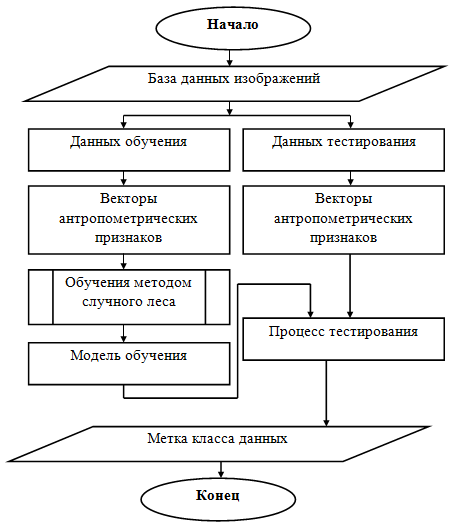
\includegraphics [scale=1] {images/h19.png}
\begin{center}
%\captionsetup{justification=justified, labelsep=period}
\caption{Предложенная модель} \label{img19}
\end{center}
\end{figure}
Архитектура системы состоит из двух основных частей. Часть $1$ используется, чтобы найти набор лучших атрибутов. Cистема генерирует наборы атрибутов, а затем использует алгоритм машинного обучения Random Forest для оценки таких наборов. Этот процесс повторяется до удовлетворения условий, чтобы остановить систему и получить набор оптимальных признаков. Часть $2$ используется, чтобы проверить подходит ли данная модель.
\subsection{Предложенный алгоритм}
В данной работе предлагается алгоритм случайного леса для классификации измерений для построения 3D модели на основе оценки и поиска набора антропометрических признаков из исходного набора признаков. Шаги выполнения алгоритма обозначается следующим образом:

\begin{itemize}
	\item \textbf{Шаг 1:} Создание $m$ наборов признаков из $n$ наборов первоначальных признаков. Каждый набор содержит $2 \frac{n}{m} $признаки. В том числе:
	
	\begin{itemize}
		\item  $\frac{n}{m}$ признаки равны;
		\item  $\frac{n}{m}$ случайные признаки.

	\end{itemize}
	
	\item \textbf{Шаг 2:} Использование Random Forest для того, чтобы вычислять оценку наборов признаков $\Rightarrow$ получение набора значений $f\left(i\right), i= \left(1,..., m\right)$;
	\item \textbf{Шаг 3:}взвешивание каждого признака $i$ рассчитывается по формуле:
	$w_j= \sum^m_{i=1}kf_i$;
	
	\begin{itemize}
		\item $k_{ij} = 0$, если признак $i$ не выбран в наборе признака $j$;
    \item $k_{ij}= 1$, если признак выбран в наборе признака $j$.
	\end{itemize}
	
	\item \textbf{Шаг 4:} Разработка нового признака включает в себя $р\%$ лучших признаков;
	\item \textbf{Шаг 5:} Повторение шага $1$ для удовлетворения одного из двух условий:
	
	\begin{itemize}
		\item Количество признаков < порога разрешено;
		\item Количество циклов определено.
	\end{itemize}
	
\end{itemize}

Изложенное выше направление рекомендуется для того, чтобы найти набор оптимальных маленьких признаков, таким образом, цель состоит в том, чтобы ограничить количество выходных признаков. Эти первоначальные признаки разделены для обеспечения всех выбранных признаков. Затем в сочетании с делением случайных признаков, создаются новые маленькие наборы признаков. Дальше алгоритм машинного обучения случайного леса используется для вычисления актуальности набора признаков. На основе значения расчетного уровня вычисления мы находим набор признаков, которые имеют меньшее количество свойств при сохранении целей работы.
\subsection{Формирование опорных точек с признаками объектной принадлежности}
В этом разделе представлен подход к реконструкции 3D-модели человека на основе антропометрических признаков, которые были извлечены и классифицированы из 2D-изображений. Мы используем набор данных  антропометрических признаков для построения 3D-модели точной и эффективной в соответствии с формой и фактическим размером объекта.

Процесс построения 3D-модели включает следующие шаги:

\begin{itemize}
	\item Шаг 1: Описание текстурных характеристик человеческого тела (кожа, волосы, лицо), а также текстуры одежды;
   \item Шаг 2: Разработка частей человеческого тела (голова, туловище, руки, ноги) с использованием ранее полученных антропометрических признаков;
\item Шаг 3: Комбинация текстуры и частей человеческого тела в блок;
\item Шаг 4: Экспорт антропометрических моделей человеческого тела в два файла: первый файл (*.mtl) описывает текстуры модели, второй файл (*.obj) содержает информацию каждой модели.
\end{itemize}

Алгоритм для соответствия 3D-модели с антропометрическими признаками:
\begin{figure}[ht!]
\centering
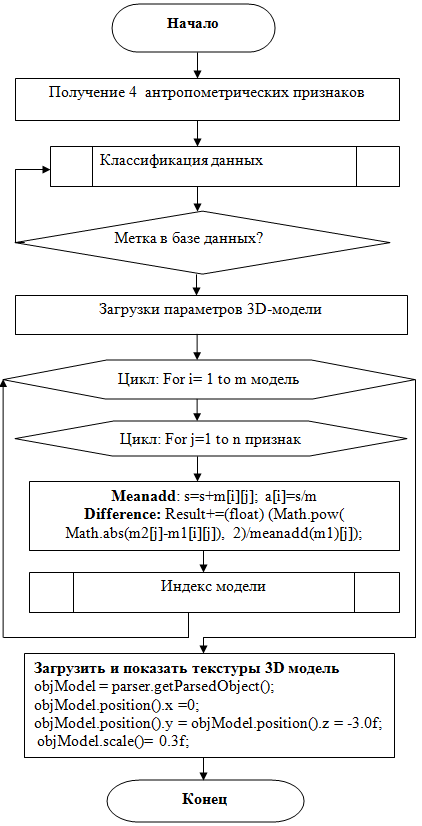
\includegraphics [scale=1] {images/h21.png}
\begin{center}
%\captionsetup{justification=justified, labelsep=period}
\caption{Алгоритм сопоставления 3D-формы с данными маркировки} \label{img21}
\end{center}
\end{figure}

\textbf{Результаты и анализ экспериментов на наборах антропометрических данных}

\textbf{Часть 1:} Обучение базового алгоритма случайного леса на наборах антропометрических данных выполнены $5$ раз с использоване библиотеки Weka \cite{Weka}. Каждый раз запуска будет диагонально выполнять проверки с количеством деревьев соответственно $100$, $200$, $300$, $400$, $500$ мы получим результат( в таблице \ref{tab5}):

\begin{table}[b!]%
\begin{center}
\caption{Результаты классификации на основе алгоритма случайного леса \cite{long1,long2}}\label{tab5}
  \begin{tabular}{|c|c|c|c|c|}
    \hline
 Количество  & Среднее   &   Стандартное   & Минимальное   & Максимальное \\
деревьев     & значение  &    отклонение   & значение      &значение      \\
\hline
100 &	0.03480	&0.025&	0.0139&	0.0606\\
\hline
200 &	0.02761	&0.0200	&0.0152	&0.0352\\
\hline
300	&0.02178	&0.0125	&0.0121	&0.0336\\
\hline
400	&0.01830	&0.0150	&0.0076	&0.0270\\
\hline
500	&0.01661	&0.0115	&0.0102	&0.0254\\
\hline

  \end{tabular}
\end{center}
\end{table}%\vspace{10mm}

\textbf{Часть 2:} Выбор набора оптимальных данных из наборов антропометрических данных мужчин первоначально предложенными методами выше. С начальным набором признаков, мы делим на m подразделение наборов признаков с использованием функции выборки <<$sample\left(, ,replace=True\right)$>> так что каждый набор содержит $\frac{n}{m}$ распределеные равномерные признаки и $\frac{n}{m}$ случайные признаки. Где $n$ - общее число признаков, $m$ - параметр распределения (в эксперименте выбрать $m=4$). В частности, файл результата <<ImportantFeature>> показывает новый набор, который включает в себя $4$ признака, расположенных соответственно в $12$ первоначальных признаках: $5,6,7,10$. С новым набором признаков, мы ещё раз выполняем часть $1$ представленную выше и получим результаты случайного леса при запуске пяти новых наборов признаков, показанных в таблице (\ref{tab6}).

\begin{table}[b!]%
\begin{center}
\caption{Результаты классификации на основе алгоритма случайного леса \cite{long1,long2}}\label{tab6}
  \begin{tabular}{|c|c|c|c|c|}
    \hline
  Количество  & Среднее   &   Стандартное   & Минимальное   & Максимальное \\
деревьев     & значение  &    отклонение   & значение      &значение      \\
\hline
100	&0.0116	&0.00833	&0.00463	&0.0202\\
\hline
200	&0.0092	&0.00667	&0.00516	&0.0117 \\
\hline
300	&0.02178	&0.00416	&0.0040	&0.0221\\
\hline
400	&0.00726	&0.0050	&0.0071	&0.009\\
\hline
500	&0.00553	&0.00383	&0.00513	&0.0085\\
\hline
  \end{tabular}
\end{center}
\end{table}%\vspace{10mm}

\subsubsection{Применение результатов классификации для построения 3D-моделей}
В работе \cite{grudinin2009} посвящена анализу антропометрических характеристик человеческого тела с целью определения границ изменения параметров и их взаимосвязи в рамках задачи параметрического моделирования компьютерных манекенов. В \cite{grudinin2014} предложен моделирование нестандартных параметризованных манекенов в рамках параметрического представления сложных геометрических объектов, удовлетворяющих заданным антропометрическим данным. Результаты исследований сосредоточены на построении частей человеческого тела: грудь и талию. Срок реализации 1-5 минут. В нашей работе используется результат классификации антропометрических данных, которые важные для построения антропологических моделей. При таком подходе, время работы программы быстрее и обеспечивает полную модель человеческого тела.

На основе выходных результатов процесса классификации - метка класса присваивается после процесса проверки. Основываясь на значении метки класса каждой записи, имеющееся $3D$-модель соответствует и подходит с параметрами каждой записи. $3D$-модели были построены при поддержке библиотек Min3D \cite{Min3D} и MakeHuman \cite{Make}. База данных включает в себя $100$ построенных моделей, в соответствии с размерами тела $XS$, $S$, $M$, $L$, $XL$. Каждый размер тела имеет $20$ моделей, построенных на основе каждого различного параметра тела.

На основе результата тестов, у нас имеется $5$ записей помеченых метками: $1$, $2$, $3$, $4$, $5$. Значит в очереди, записи имеют $3D$-модели соответствующие размерам $XS$, $S$, $M$, $L$, $XL$. Выбор наиболее подходящей модели для каждой записи будет основываться на $4$ признаках, которые выбраны из предлагаемого алгоритма: обхват груди $\left(B\right)$, обхват талии $\left(W\right)$, обхват бедер $\left(C\right)$, рост $\left(H\right)$. Мы создаем формулу для расчета следующим образом:
\begin{equation}\label{eq26}
Model = Min\left\{\sum^N_{i=1}\left(B-B_i\right)^2+\left(C-C_i\right)^2+\left(W-W_i\right)^2+\left(H-H_i\right)^2\right\}.
\end{equation}
Применение результатов алгоритма классификации случайного леса повышает точность результатов и уменьшает время вычисления в программе. График сравнения среднего времени при запуске случайного леса $5$ раз на новые наборы и начальные наборы антропометрических данных с количеством деревьев соответственно $100$, $200$,$300$, $400$, $500$ (рис. \ref{img20}).
\begin{figure}[ht!]
\centering
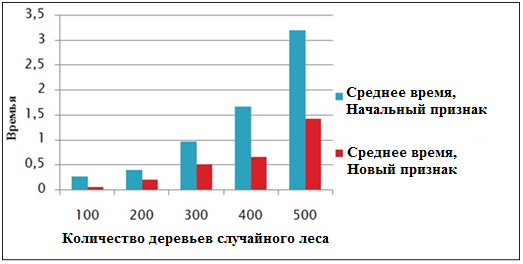
\includegraphics [scale=1] {images/h20.png}
\begin{center}
%\captionsetup{justification=justified, labelsep=period}
\caption{Время работы классификации для каждого набора данных.} \label{img20}
\end{center}
\end{figure}
%-------------------------
\section{Основные результаты и выводы по главе 2}

\begin{enumerate}
	\item Предложен метод извлечения антропометрических признаков на изображениях и видео на основе алгоритмов компьютерного зрения. Проведено улучшение качества изображения с помощью технической обработки изображений, обнаружение объектов с помощью алгоритма вычитания фона, сегментации изображения с помощью алгоритма разреза на графах, извлечения ключевых точек методом $ICP$;
 \item Предложен метод поправочного множителя с использованием комбинированного алгоритма $ICP$ для повышения точности извлечения антропометрических признаков на изображениях и видео.
\item Предложен метод классификации антропометрических данных с помощью алгоритма случайных лесов - Random Forest для классификации размеров и $3D$ моделей человеческого тела.
\item Предложена модель классификации Wrapper и алгоритм извлечения важных признаков для повышения точности и скорости алгоритма случайного леса.
\item Разработан алгоритм и схема его применения для извлечения и классификации антропометрических данных с помощью алгоритмов компьютерного зрения.
\item На основе численных экспериментов проведен сравнительный анализ применимости и сравнение возможности применения алгоритмов компьютерного зрения в антропометрии - обнаружение объектов с помощью алгоритма вычитания фона, сегментации изображения с помощью алгоритма разреза графов, извлечения ключевых точек методом $ICP$, классификации антропометрических данных с помощью алгоритма случайных лесов для решения проблемы в  антропометрии на статических изображениях в присутствии шума. 
\item Экспериментальные результаты представлены в таблицах (\ref{tab1}), (\ref{tab3}), (\ref{tab5}), (\ref{tab6}) показывают, что алгоритмы работают с высокой скоростью и точностью при извлечении и классификации антропометрических данных на изображениях и на видеопоследовательностях в присутствии шума и в реальном режиме времени. 

\end{enumerate}

%-------------------------

           % Глава 1
%\chapter{Нелинейные интегральные уравнения Вольтерра I рода с кусочно-непрерывными ядрами} \label{chapt2}
%\chapter{Интегральные модели Вольтерра на основе нелинейных уравнений} \label{chapt2}
%\chapter{Интегральные модели развивающихся динамических систем на основе нелинейных уравнений Вольтерра I рода с разрывными ядрами} \label{chapt2}
%\section{Интегральные модели развивающихся динамических систем на основе нелинейных уравнений Вольтерра I рода с разрывными ядрами} \label{chapt2}


%\section{Постановка задачи} \label{sect2_1}
\chapter{Системный анализ и проектирование построения систем компьютерного зрения в антропометрии. Тестирование и разработка алгоритмов компьютерного зрения на изображении и видео}
В данной главе приводятся информация о анализе, проектировании и построении антропометрического пакета прикладных программ с помощью  объектно-ориентированного языка UML. При анализе результатов испытаний применяются алгоритмы компьютерного зрения в условиях шума, и в режиме реального времени.


\section{Анализ и проектирование системы компьютерного зрения в антропометрии}
Жизненный цикл программы в целом не может быть разделен на периоды. Он описывает процесс создания, тестирования и поддержания работы системы \ref{img33}.

\begin{figure}[ht!]
\centering
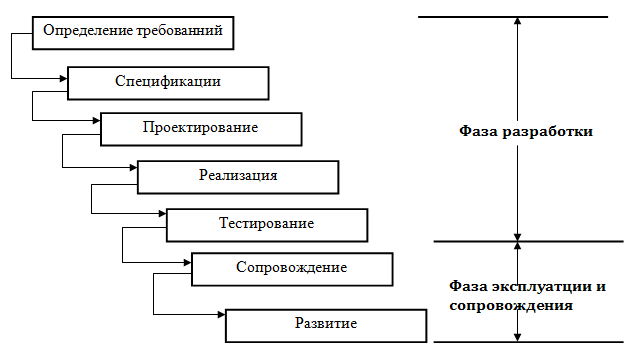
\includegraphics [scale=1] {images/h33.png}
\begin{center}
%\captionsetup{justification=justified, labelsep=period}
\caption{Общепринятая модель жизненного цикла программного обеспечения.} \label{img33}
\end{center}
\end{figure}

В данной работе подробно описан этап проектирования системы. Для этого было создано хранилище документов проекта, включающее в себя: теории и модели, методы и инструменты, используемые для создания и развития системы. Анализ и проектирование системы основаны на двух факторах: 

\begin{itemize}
	\item Понимание целей, структуры и процессов работы системы;
  \item Применение передовых методов и соответствующих алгоритмов для повышения эффективности работы и точности системы.

\end{itemize}
Особенностью анализа и объектно-ориентированного проектирования является система, включающая в себя совокупность объектов, взаимодействующих друг с другом для выполнения задачи с  достижением более высоких результатов. Для достижения этой цели мы должны использовать системные модели объектов со следующими основными характеристиками:

\begin{itemize}
	\item С высокой абстракцией;
  \item По состоянию упаковочной информации;
  \item Модуль;
  \item Наследование.

\end{itemize}
Сегодня UML является инструментом, обладающим  всеми характеристиками и условиями,о которых говорилось выше, для построения модели объекта. UML - графический язык для документирования, конструирования, описания параметров и визуализации абсолютно различных систем (программ в частности).
Графики моделирования объектов представлены в диссертации, в том числе:

\begin{itemize}
	\item \textbf{Диаграмма прецедентов} (Use Case diagram) - диаграмма, отражающая отношения между актёрами и прецедентами, являющаяся составной частью модели прецедентов, позволяющей описать систему на концептуальном уровне;
\item \textbf{Диаграмма классов} (Static Structure diagram) - диаграмма, демонстрирующая классы системы, их атрибуты, методы и взаимосвязи между ними. Входит в UML;
\item \textbf{Диаграмма последовательности} (sequence diagram): диаграмма, на которой для некоторого набора объектов на единой временной оси показан жизненный цикл (создание-деятельность-уничтожение) и взаимодействие (отправка запросов и получение ответов). Используется в языке UML.

\end{itemize}

Объектная модель описывает структуру объектов, их операции, атрибуты  и взаимосвязи с другими объектами. Объектная модель показывает понятия и реальные объекты, которые важны для разрабатываемой системы. Цель разработки объектной модели - выделение и описание объектов, составляющих проектируемую систему и выявление различных зависимостей между объектами.

Система компьютерного зрения в антропометрии включает в себя следующие основные вопросы:

\begin{itemize}
	\item Сбор и обработка данных с камеры;
	\item Извлечение антропометрических признаков;
	\item Классификация антропометрических данных;
	\item Разработка приложений для текстильной промышленности (E-Tailor) и фитнеса (E-фитнес) на основе результатов системы компьютерного зрения в антропометрии.
\end{itemize}

\begin{figure}[ht!]
\centering
\includegraphics [scale=0.4] {images/h35.png}
\begin{center}
\caption{Структура ПО} \label{img35}
\end{center}
\end{figure}

\subsection{Анализ и проектирование системы компьютерного зрения в антропометрии для текстильной промышленности}

\textbf{Цель}: Описание работы программы автоматического измерения размеров человеческого тела, 3D моделирование тела мужчины / женщины, выбор размеров одежды на основе антропометрических признаков.

Система состоит из одного главного фактора: пользователи. Система имеет основные функции:

\begin{itemize}
	\item Сбор данных с камеры;
	\item Заполнение информации о росте, весе;
	\item 3D-моделирование человеческого тела;
	\item Классификация и предсказание размеров одежды;
	\item Контакты с командой разработчиков.

\end{itemize}
\begin{figure}[ht!]
\centering
\includegraphics [scale=0.5] {images/h22.png}
\begin{center}
%\captionsetup{justification=justified, labelsep=period}
\caption{Диаграмма прецедентов - использование системы компьютерного зрения приложения E-Tailor.} \label{img22}
\end{center}
\end{figure}
\begin{figure}[ht!]
\centering
\includegraphics [scale=0.5] {images/h23.png}
\begin{center}
%\captionsetup{justification=justified, labelsep=period}
\caption{Диаграмма классов - система компьютерного зрения в антропометрии приложения E-Tailor.} \label{img23}
\end{center}
\end{figure}
\begin{figure}[ht!]
\centering
\includegraphics [scale=0.8] {images/h28.png}
\begin{center}
%\captionsetup{justification=justified, labelsep=period}
\caption{Диаграмма последовательности - система компьютерного зрения в антропометрии приложения E- Tailor.} \label{img28}
\end{center}
\end{figure}

\subsection{Анализ и проектирование системы компьютерного зрения в антропометрии для фитнеса}
\textbf{Цель}: Описание работы программы автоматического измерения размеров человеческого тела, 3D моделирование тела мужчины / женщины, автоматизация измерения индекса массы тела (ИМТ), анализ антропометрических признаков по стандартам фитнеса.

Система состоит из одного главного фактора: пользователи. Система имеет основные функции:

\begin{itemize}
	\item Сбор данных с камеры;
	\item Заполнение информации о росте, весе;
	\item 3D-моделирование человеческого тела;
	\item Анализ антропометрических признаков по стандартам фитнеса;
	\item Анализ ожирения в соответствии с индексом ИМТ;
	\item Тренажерные упражнения фитнеса в домашних условиях;
	\item Контакты с командой разработчиков.

\end{itemize}
\begin{figure}[ht!]
\centering
\includegraphics [scale=0.5] {images/h25.png}
\begin{center}
%\captionsetup{justification=justified, labelsep=period}
\caption{Диаграмма прецедентов - использование системы компьютерного зрения приложения E-Fitness.} \label{img25}
\end{center}
\end{figure}
\begin{figure}[ht!]
\centering
\includegraphics [scale=0.5] {images/h26.png}
\begin{center}
%\captionsetup{justification=justified, labelsep=period}
\caption{Диаграмма классов - система компьютерного зрения в антропометрии приложения E- Fitness.} \label{img26}
\end{center}
\end{figure}
\begin{figure}[ht!]
\centering
\includegraphics [scale=0.8] {images/h27.png}
\begin{center}
%\captionsetup{justification=justified, labelsep=period}
\caption{Диаграмма последовательности - система компьютерного зрения в антропометрии приложения E- Fitness.} \label{img27}
\end{center}
\end{figure}
%-------------------------
\section{Тестирование и разработка алгоритмов компьютерного зрения на изображении и видео}
\subsection{Эксперимент}
Цель эксперимента состояла в том, чтобы проверить эффективность работы алгоритмов, методов компьютерного зрения в антропометрии, проверить обоснованность конструкции системы, учитывая влияние внешних факторов на точность алгоритма.

Система компьютерного зрения в антропометрии состоит из 3 основных частей: извлечение антропометрических признаков, классификация антропометрических признаков и применения их на практике. 

Процесс извлечения  антропометрических признаков выполняется следующим образом. Во-первых, происходит обнаружение и распознавание объектов методами вычитания фона и обнаружения лица человека. Следующим шагом является сегментация и определение ключевых точек с помощью метода разреза на графах (Graph cuts) и итеративного алгоритма ближайших точек (Iterative Closest Point - ICP). Процесс классификации антропометрических признаков состоит из двух частей: обучение и тестирование. Важным шагом в этом процессе является  создание учебной модели для классификации новых данных с высокой точностью. 

В данной работе рассматривается построение приложения компьютерного зрения в антропометрии для двух областей: пошив одежды и фитнес-тестирование. В этом разделе рассматривается возможность создания 3D-моделей, классифиции размеров человеческого тела, способность анализировать антропометрические данные в соответствии со стандартом IBM, Fitness и т.д. Также, сравнивается наш метод и алгоритм построения системы компьютерного зрения антропометрии и другие алгоритмы, чтобы найти подходящий для успешной реализации.

\subsection{Тестирование разработанного ПО – извлечение и классификация антропометрических признаков на видео}
Эксперимент проводился на основе языка C ++ (Visual Studio 2010), Java, Matlab с использованием открытой библиотеки компьютерного зрения - OpenCV, библиотеки моделирования 3D для компьютеров и смартфонов - Min3D и библиотеки дизайн 3D моделей - Humanmaker. 

\textbf{Оборудование тестирования:}

\begin{itemize}
	\item Ноутбук с процессором Intel Core 2 Duo (2.3 ГГц), 3 Гб оперативной памяти, камера 1,3 мегапикселей, которая передает 30 кадров в секунду с разрешением  $320 * 240$ пикселей;
	\item Смартфон Самсунг с фронтальной камерой 5 мегапикселей.

\end{itemize}
Эксперимент проводился на основе данных, собранных с помощью личного устройства. На этапе сбора данных пользователь стоит перед фронтальной камерой телефона (расстояние такое, чтобы тело полностью было в кадре), выполняется серия движений, поворот на 90 градусов налево, направо и наоборот. Первоначально будут собираться данные с изображения. Приложение идентифицирует объект, который появляется в кадре и определяет, человек это или нет (на основе обнаружения лица). Затем программа автоматически собирает и выполняет вычитание фона изображения, сегментацию частей человеческого тела, определяет ключевые точки на теле. Происходит калибровка для расчета антропометрических признаков.

Для проверки правильности работы программы, эксперименты проводились несколько раз для одного и того же объекта, в разном времени и месте, в различных условиях шума и освещения, таких как, эксперименты \ref{img29}.

\begin{figure}[ht!]
\centering
\includegraphics [scale=0.1] {images/h29.png}
\begin{center}
%\captionsetup{justification=justified, labelsep=period}
\caption{Пример данных эксперимента.} \label{img29}
\end{center}
\end{figure}

База данных для экспериментов на компьютере состоит из 6 видео. Эта база данных была создана, чтобы получить данные для тестирования и оценки эффективности работы методов и алгоритмов компьютерного зрения на видео. Создание этой базы необходимо, чтобы учитывать влияние различных факторов на производительность системы (\ref{img36}), (\ref{img37}).

\begin{figure}[ht!]
\centering
\includegraphics [scale=0.5] {images/h36.png}
\begin{center}
%\captionsetup{justification=justified, labelsep=period}
\caption{Результаты извлечения антропометрических признаков и 3D-моделей для женщин.} \label{img36}
\end{center}
\end{figure}
\begin{figure}[ht!]
\centering
\includegraphics [scale=0.5] {images/h37.png}
\begin{center}
%\captionsetup{justification=justified, labelsep=period}
\caption{Результаты извлечения антропометрических признаков и 3D-моделей для мужчин.} \label{img37}
\end{center}
\end{figure}

В ходе эксперимента были использованы алгоритмы компьютерного зрения и извлечения антропометрических признаков. Для этого используются алгоритмы разреза на графах, а также итеративные алгоритмы ближайших точек двух видов: из 24 ключевых точек и 28 ключевых точек для сравнения результата алгоритма вычитания фона и метода выпуклой оболочки \ref{tab7} . В нашей работе \cite{long1} изложен метод измерения различных антропометрических признаков на основе анализа цифровых изображений. Для более эффективного измерения признаков предлагается использовать субпиксельную обработку и анализ выпуклой оболочки. В нашем подходе контур тела описывается выпуклостью дефектов треугольников. Тела представлены треугольниками. Такие треугольники имеют три координаты: выпуклый дефект старт, выпуклый дефект конец, и выпуклый дефект положения точек, соответственно помечены. Мы определили области интересов, которые содержат части тела. Таким образом, мы получили 5 выпуклых областей с соответствующими условиями.

\begin{table}[b!]%
\begin{center}
\caption{Результаты извлечения антропометрических признаков}\label{tab7}
\begin{tabular}{ |c|c|c|c| } 
\hline
  \multirow{3}{*}& Graph-cuts + ICP  & Graph-cuts + ICP  &Вычитание фона \\
								 & (28 ключевых - &(24 ключевых - & + выпуклая\\
	               & - точек)       & - точек)      & оболочка\\
\hline
\multirow{2}{*}{Груди} & \multicolumn{3}{|c|}{93}\\ 
                         & 92.85 & 90.75&85.0 \\ 
\hline
\multirow{2}{*}{Талия} & \multicolumn{3}{|c|}{75}\\ 
                         & 74.80 & 72.0 & 69.79 \\ 	
\hline
\multirow{2}{*}{Бедра} & \multicolumn{3}{|c|}{91}\\ 
                         & 91.3 & 89.65 & 88.65 \\ 
\hline
\multirow{2}{*}{Длина рук} & \multicolumn{3}{|c|}{50}\\ 
                         & 50.40 & 47.62 & 40.30 \\
\hline
\multirow{2}{*}{Обхват } & \multicolumn{3}{|c|}{29}\\ 
                бицепса  & 28.50 & 27.31 & 32.50\\
\hline
\multirow{2}{*}{Обхват } & \multicolumn{3}{|c|}{36}\\ 
                 шеи        & 36.21 & 35.70 & 38.95\\	
\hline
\multirow{2}{*}{Длина } & \multicolumn{3}{|c|}{40}\\ 
                 спины        & 40.10 & 38.75 & 56.50\\	
\hline
\multirow{2}{*}{Ширина } & \multicolumn{3}{|c|}{36}\\ 
                  плеча       & 36.25 & 34.30 & 31.90\\
\hline
\multirow{2}{*}{Длина } & \multicolumn{3}{|c|}{13}\\ 
                 плеча        & 13.10 & 12.83 & 15.56\\
\hline
\end{tabular}
\end{center}
\end{table}%\vspace{10mm}

В (рис. \ref{img24}) описан результат эксперимента проверки точности извлечения антропометрических признаков 3 методов (разреза на графах + ICP для 28 опорных точек, разреза на графах + ICP для 24 опорных точек, вычитание фона + выпуклая оболочка) с ручной метода для одного человека.

\begin{figure}[ht!]
\centering
\includegraphics [scale=0.8] {images/h24.png}
\begin{center}
%\captionsetup{justification=justified, labelsep=period}
\caption{Сравнение результата эксперимента.} \label{img24} \label{img24}
\end{center}
\end{figure}

%-------------------------
\section{Основные результаты и выводы по главе 3}

\begin{enumerate}
	\item В этой главе описывается анализ проектирования систем компьютерного зрения в антропометрии для практических применений: пошив одежды и фитнес-тестирование с помощью аналитических методов объектно-ориентированного UML. Используются диаграммы прецедентов, диаграммы классов и диаграммы последовательности. Классы подробно анализируются, с указанием задач каждой компоненты в программе. Также обоснована целесообразность проектирования приложений компьютерного зрения;
	\item Описаны результаты тестирования алгоритмов компьютерного зрения, в том числе предварительной обработки изображений с помощью фильтра Гаусса, эквализация гистограммы, алгоритм вычитания фона изображения на основе фоновых модели, алгоритм сегментации изображений методом разреза на графах (graph cuts), итеративный алгоритм ближайших точек (Iterative Closest Point - ICP). Алгоритмы функционируют в режиме реального времени и в условиях наличия с шумов в видеопоследовательностях. Эксперименты доказали, что предложенные алгоритмы эффективно работают и включают в себя: извлечение и классификация антропометрических признаков;
	\item Проведен анализ практических результатов экспериментов извлечения антропометрических признаков. Проведено сравнение результатов предложенных методов с методом выпуклой оболочки и вычитания фона по точности. Доказывается преимущество приведенного алгоритма на основе метода разреза графа и итеративного алгоритма ближайших точек;
	\item Результаты экспериментов по классификации антропометрических данных на компьютере и смартфоне показали, что алгоритм случайного леса эффективно работает для решения задач классификации в видеопоследовательностях в режиме реального времени;
	\item Сравнение результатов классификации между алгоритмом случайного леса и алгоритмом Boosting, работающими с видео, показало, что по точности и времени выполнения, более результативный алгоритм случайного леса для системы компьютерного зрения в антропометрии. Алгоритм случайного леса полностью совместим с визуальной системой.
\end{enumerate}

%-------------------------           % Глава 2
%\chapter{Применение разработанных алгоритмов} \label{chapt3}
%\chapter{Дифференцирование зашумленных функций} \label{chapt3}
%\chapter{Применение интегральных уравнений для решения практических задач} \label{chapt3}
%\chapter{Приложение интегральных моделей в задаче составления графиков  аккумулирования и генерации электроэнергии} \label{chapt3}
\chapter{Приложение «Measure Me» - система компьютерного зрения в антропометрии на операционной системе Андроид для смартфона} \label{chapt3}
В этой главе представлены разработки приложений системы компьютерного зрения в антропометрии на практике. Приложение разработано для операционной системы Андроид. Также приведем описание библиотек и инструментов поддержки для разработки прикладного программного обеспечения «Measure Me».
\section{Средства поддержки для разработки программного обеспечения (ПО) на смартфоне}
\subsection{Среда разработки приложений – операционная система Андроид}
Android (Андроид) — операционная система для смартфонов, интернет-планшетов, электронных книг, цифровых проигрывателей, наручных часов, игровых приставок, нетбуков, смартбуков, очков Google, телевизоров и других устройств. В будущем планируется поддержка автомобилей и бытовых роботов. Основана на ядре Linux и собственной реализации виртуальной машины Java от Google. В 86\% смартфонов, проданных во втором квартале 2014 года, была установлена операционная система Android. При этом за 2014 год было продано более 1 миллиарда Android-устройств \cite{android}.

\textbf{Преимущества операционной системы Android:}

\begin{itemize}
	\item Операционная система с открытым исходным кодом обладает большими преимуществами в возможностях настройках, и имеет возможность дополнительно редактировать код без вмешательства или ограничений от Google;
	\item Большинство мобильных компаний выбирают  Android для своих продукций, руководствуясь разумной ценой;
	\item Android включает в себя большой онлайн-магазин приложений Google Play; 
	\item Удобный и простой в использовании;
	\item Возможность работать в многозадачном режиме.

\end{itemize}

\textbf{Недостатки операционной системы Android:}

\begin{itemize}
	\item Легкое заражение вредоносными программами и вирусами. Из-за того, что программное обеспечение с открытым исходным кодом качество операционной системы не контролируется и имеются небезопасные приложения в Google Play;
	\item Большая фрагментация. От высококачественных Android устройств, таких как Galaxy S6, Galaxy Note 4, Xperia Z4 и т.д., до некачественных;
\item Обновления появляются не для всех устройств. Когда выпускается новая версия операционной системы, не все продукты находятся в актуальном состоянии, если мы хотим испытать новую версию ОС, то надо купить новое оборудование.

\end{itemize}
Также: открытый исходный код и возможность изменения Android делают возможным появление на других электронных устройствах, таких как ноутбуки и нетбуки, смартбуки, смарт-телевизоры и фотоаппараты. Кроме того, операционная система Android также применяется в смарт-очках (Project Glass), часах, наушниках, портативных музыкальных плеерах, настольных телефонах и игровых машинах.
\subsection{Среда программирования для Android}
Официальный язык программирования Android - Java. Хотя приложения для Android были разработаны на основе платформы Java, они не поддерживают J2ME и J2SE (два популярных языка программирования для мобильных устройств).

Android SDK включает в себя отдельные инструменты, такие как отладчик, библиотеки, эмулятор телефона Android, документы поддержки и примеры кода. Android в настоящее время предлагает инструменты для нескольких операционных систем (Windows, Linux, Mac и прочие), в виде пакета средств разработки Java (JDK), Apache Ant и Python 2.2 старше.

Основной средой программирования (IDE) для Android является Eclipse (начиная с версии 3.2) с поддержкой Plugin Android Development Tools (ADT). Тем не менее, программисты могут использовать любой IDE или текстовый редактор для написания Java-код, а затем скомпилировать XML и собрать приложение с помощью инструментов командной строки.

Android приложения упаковываются в .apk файл и хранятся в папке  /data/app  ОС Android. Некоторые типичные инструменты поддержки программирования на Android: SQLite Manager, DroidDraw, Balsamiq Mockups и AdobeFireworks, StarUML.

\textbf{Основные компоненты проекта Android на Eclipse:}


\begin{itemize}
  \item app/build/ - директория для хранения результатов сборки;
	\item app/libs/ – библиотеки;
	\item app/src/ – исходный код проекта;
	\item app/src/main/java – Java-классы;
	\item app/src/ – исходный код проекта;
	\item app/src/main/res – ресурсы ;
	\item app/src/main/AndroidManifest.xml – файл Android Manifest.
\end{itemize}

\begin{figure}[ht!]
\centering
\includegraphics [scale=1] {images/h30.png}
\begin{center}
%\captionsetup{justification=justified, labelsep=period}
\caption{Структура директории и файлов проекта ПО Андроид на Eclipse} \label{img30}
\end{center}
\end{figure}
\textbf{Файл AndroidManifest.xml:}

Этот файл является основой всех Android-приложений, AndroidManifest.xml файл помещается в папке Root и показывает компоненты, которые включены в приложении (activities, services) и как компоненты прикреплены вместе.

При создании файла manifest, необходимо обеспечить свойства пакета, то есть имя пакета Java, используемого в качестве основы для нашего приложения. После ввода имени пакета и, в случае необходимости, в файле manifest, мы можем сократить, например, с классом "com.yourapp.android.search. Someclass", просто пишется: ".Someclass".
\begin{figure}[ht!]
\centering
\includegraphics [scale=1] {images/h34.png}
\begin{center}
%\captionsetup{justification=justified, labelsep=period}
\caption{Структура файла Manifest.} \label{img34}
\end{center}
\end{figure}

\subsection{Библиотеки поддержки для разработки приложений}
\textbf{Библиотека обработки изображений для Android – OpenCV}

OpenCV (Open Computer Vision Library) - библиотека компьютерного зрения, которая распространяется в виде открытого исходного кода. Изначально OpenCV была написана для программ на языке C, но теперь работает на других языках, таких как C ++, Java, Android, IOS. А так же время поддерживает много ОС: Windows, Linux, Android, Mac OS, Cube.

В настоящее время в библиотеке OpenCV существует более 2500 алгоритмов, которые включают в себя совокупность всех алгоритмов компьютерного зрения и машинного обучения. Эти алгоритмы могут быть использованы для обнаружения и распознавания лиц, распознавания объектов и классификации человеческих действий в видео, отслеживать перемещение объектов, извлекать 3D модели объектов, нахождения похожих изображений из базы данных изображений, удаления эффекта красных глаз из изображений, снятых с использованием вспышки, отслеживания движения глаз и т.д.

Структура OpenCV включает в себя 4 основных компонента:
\begin{figure}[ht!]
\centering
\includegraphics [scale=1] {images/h31.png}
\begin{center}
%\captionsetup{justification=justified, labelsep=period}
\caption{Структура OpenCV} \label{img31}
\end{center}
\end{figure}


\begin{itemize}
	\item \textbf{CxCore}: Содержит основную структуру, такие как точки, линии, блоки, руки, матриц, и связанные с ними манипуляции низкого уровня;
	\item \textbf{MLL} (Machine Learning Library) является библиотекой машинного обучения, эта библиотека включает в себя много классов статистики и инструментов обработки;
	\item \textbf{CV} (Computer Vision – компьютерное зрение): Содержит множество операций, связанных с обработкой изображений низкого уровня, таких как фильтрация изображений, обнаружение контура, преобразование Фурье и прочее;
	\item \textbf{HighGUI}: Работа с файлами изображений и видео, такие как загрузка изображения, отображения изображений, преобразование форматов.
\end{itemize}
\textbf{Open CV имеет следующие основные модули}:

\begin{itemize}
	\item Opencv core: основная функциональность. Включает в себя базовые структуры, вычисления, ввод и вывод для XML и т.д;
	\item Opencv imgproc: обработка изображений;
	\item Opencv highgui: модуль для создания пользовательского интерфейса;
	\item Opencv feature2d: распознавание и описание плоских примитивов (SURF, FASR и др.);
	\item Opencv video:анализ движения и отслеживание объектов;
	\item Opencv objdetect: обнаружение объектов на изображении;
	\item Opencv ml:модели машинного обучения.	
\end{itemize}

\textbf{Библиотека моделирования 3D – MakeHuman}

MakeHuman - программное обеспечение с открытым исходным кодом, является бесплатным, служит для создания 3D модели человека. MakeHuman прост в использовании и имеет интуитивно понятные параметры, в том числе:

\begin{itemize}
	\item Возраст, пол, рост, вес;
	\item Пропорция тела, форма лица;
	\item Глаза, нос, рот, подбородок, уши, шея ...
	\item Руки, ноги

\end{itemize}

Это приложение разработано с использованием 3D-технологий. Создание начинается с формы человека, а затем преобразуется во множество различных персонажей, в том числе мужчин и женщин. Кроме того, мы можем преобразовать 3D модели из формы ребенка в юношу, взрослого и пожилого человека. Начиная с первой версии, MakeHuman использовало уникальные сетки.  

\textbf{Библиотека поддержки моделирования min3D}
\begin{figure}[ht!]
\centering
\includegraphics [scale=1] {images/h32.png}
\begin{center}
%\captionsetup{justification=justified, labelsep=period}
\caption{Структура библиотеки моделирования min3D} \label{img32}
\end{center}
\end{figure}

Библиотека Min3D имеет открытый исходный код, разработанный для операционной системы Android для отображения 3D-моделей. Она использует инструмент поддержки OpenGL версий 1.0/1.1. Min3D совместим с OpenGL API, предоставляет удобную и полезную библиотеку для приложений моделирования. Библиотека Min3D легко восстановит 3D-модели объекта. Min3D работает на следующих файлах: Wavefront OBJ, 3DS, MD2.

В данной работе используется сочетание двух библиотек MakeHuman и Min3D для создания шаблонов 3D-моделей человеческого тела. Эти шаблоны описаны в двух файлах с расширениями *.mtl и *.obj. Эти файлы хранятся в папке Андроида (project/res/raw). 


\begin{itemize}
	\item Файлы *.obj содержат данные, описывающие 3D-модели в формате текста, а также другую информацию об объекте. Файлы *.obj просты в использовании и полезны для хранения и отображения 3D-модели любого объекта;
	\item Файлы *.mtl содержат информацию текстур объектов. 
\end{itemize}
Оба файла * .obj и * .mtl являются конечным результатом конструкции 3D-модели человека на основе результата извлечения антропометрических признаков системы компьютерного зрения, предложены библиотека MakeHuman и входные данные для отображения на устройствах Android сгенерированные с помощью библиотеки min3D.





%-------------------------
\section{Программное обеспечение системы компьютерного зрения в антропометрии}
Приложение создано для обработки видео на смартфонах, оно основано на алгоритмах компьютерного зрения в антропометрии с использованием поддержки среды Android и библиотек OpenCV, Min3D, MakeHuman. В данной диссертации применяется система компьютерного зрения в антропометрии для создания приложений в областях пошива одежды (E-Tailor) и фитнеса (E-Fitness). Приложения загружены на онлайн-магазин GooglePlay и их можно скачать бесплатно. Системные требования: версия Android от 4.4.2, передняя камера с разрешением 2.0 мп или выше.

После загрузки и установки, система автоматически загрузит и установит библиотеку OpenCV для телефона.

\subsection{Применение системы компьютерного зрения в антропометрии для пошива одежды (E-Tailor)}
Программа <<E-Taloir>> предназначена для пошива одежды.
При запуске программы появляется главное окно формы \ref{img42}

\begin{itemize}
\item <<Measure Me>> В рабочей области отображается видеопоследовательность, область обнаружения объектов и извлечение антропометрических признаков;
\item <<Credit>> Контакты с командой разработчиков;
\item <<Exit>> Позволяет осуществить выход из программы.
\end{itemize}

\begin{figure}[ht!]
\centering
\includegraphics [scale=0.5] {images/h42.png}
\begin{center}
%\captionsetup{justification=justified, labelsep=period}
\caption{Основный интерфейс приложения E-Tailor} \label{img42}
\end{center}
\end{figure}
\textbf{Основные функции приложения E-Tailor \ref{img43}}

\begin{itemize}
	\item Позволять пользователям добавлять информацию;
	\item Показать 3D-модель на основе антропометрических признаков и классификации данных;
	\item Позволять пользователям выбрать марки одежды и классифицировать размеры одежды.
\end{itemize}

\begin{figure}[ht!]
\centering
\includegraphics [scale=0.5] {images/h43.png}
\begin{center}
%\captionsetup{justification=justified, labelsep=period}
\caption{Результат функции выбора размеров одежды} \label{img43}
\end{center}
\end{figure}


%-------------------------
\subsection{Применение системы компьютерного зрения в антропометрии для фитнеса (E-Fitness)}
Программа <<E-Fitness>> предназначена для фитнеса.
При запуске программы появляется главное окно формы \ref{img38}

\begin{itemize}
\item <<Measure Me>> В рабочей области отображается видеопоследовательность, область обнаружения объектов и извлечение антропометрических признаков;
\item <<Credit>> Контакты с командой разработчиков;
\item <<Exit>> Позволяет осуществить выход из программы.
\end{itemize}

\begin{figure}[ht!]
\centering
\includegraphics [scale=0.5] {images/h38.png}
\begin{center}
%\captionsetup{justification=justified, labelsep=period}
\caption{Основный интерфейс приложения E-Fitness} \label{img38}
\end{center}
\end{figure}

\textbf{Основные функции приложения E-Fitness}\ref{img39}

\begin{itemize}
	\item Позволять пользователям добавлять информацию;
	\item Показать 3D-модель на основе антропометрических признаков и классификации данных \ref{img40};
	\item Анализ антропометрических признаков на основе стандартов Fitness \ref{img41}.
\end{itemize}

\begin{figure}[ht!]
\centering
\includegraphics [scale=0.5] {images/h39.png}
\begin{center}
%\captionsetup{justification=justified, labelsep=period}
\caption{Интерфейс работы программы } \label{img39}
\end{center}
\end{figure}

\begin{figure}[ht!]
\centering
\includegraphics [scale=0.5] {images/h40.png}
\begin{center}
%\captionsetup{justification=justified, labelsep=period}
\caption{Результат 3D-моделей} \label{img40}
\end{center}
\end{figure}
В (рис.\ref{img41}) описывает анализ антропометрических признаков по фитнес-стандартам. Где красная линия - реальные размеры, зеленная линия - размеры по фитнес-стандартам. Приложение позволяет пользователям сравнить свои параметры с размерами по фитнес-стандартам.  
\begin{figure}[ht!]
\centering
\includegraphics [scale=0.5] {images/h41.png}
\begin{center}
%\captionsetup{justification=justified, labelsep=period}
\caption{Результат анализа антропометрических признаков на основе стандартам Fitness} \label{img41}
\end{center}
\end{figure}
%-------------------------
%-------------------------
\subsection{Основные результаты и выводы по главе 4}

\begin{enumerate}
	\item Описание среды разработки приложения Android, библиотек поддержки алгоритмов компьютерного зрения OpenCV, поддержки построения 3D-моделей человеческого тела MakeHuman и библиотеки поддержки 3D для Android – Min3D;
	\item Описание и инструкция для скачивания программы. Инструкция конфигурации библиотеки OpenCV с Android.
	\item Разработка приложения компьютерного зрения в антропометрии для пошива одежды (E-Tailor). Главные функции: автоматизация извлечения антропометрических признаков и классификация размеров одежды;
	\item Разработка приложения компьютерного зрения в антропометрии для фитнеса (E-Fitness). Главные функции: автоматизация извлечения антропометрических признаков, построение 3D-моделей человеческого тела, анализ и сравнение признаков по телосложению, индексу массы тела (ИМТ);
	\item Приложения разработаны на ОС Android для смартфонов и на основе методов и алгоритмов компьютерного зрения для извлечения и классификации антропометрических признаков. Программный модуль имеет простой, удобный и интуитивно понятный интерфейс.
\end{enumerate}

%-------------------------           % Глава 3
\chapter*{Заключение}
\addcontentsline{toc}{chapter}{Заключение}
%\Conclusion
В данной диссертации решены практические задачи научно-технических исследований и разработок алгоритмов компьютерного зрения в антропометрии на изображении и видео.

В диссертации выполнены работы и получены научно-практические результаты. Основные выводы заключаются в следующем:

\begin{enumerate}
	\item Исследование и разработка алгоритмов компьютерного зрения для  извлечения антропометрических признаков на изображении и видео, основанные на комбинации алгоритмов сегментации изображений разреза на графах (Graph-cuts) и итеративного алгоритма ближайших точек (ICP), построение множества ключевых точек объектов;
	\item Предложена модель и разработка алгоритма классификации данных методом случайного леса (Random Forest) для приложения, которое классифицирует объекты на основе антропометрических признаков;
	\item Разработка алгоритмов и методов компьютерного зрения в антропометрии на изображениях и видео с наличием шума и в режиме реального времени;
	\item Построение антропометрических 3D-моделей человеческого тела на основе результата извлечения антропометрических признаков;
	\item Развитие системы компьютерного зрения в антропометрии для смартфонов на ОС Android;
	\item Разработать и обеспечить полезные приложения для жизни: приложение «E-Tailor» для текстильной промышленности и приложение «E-Fitness» для фитнеса.
\end{enumerate}



      % Заключение
\clearpage                                  % В том числе гарантирует, что список литературы в оглавлении будет с правильным номером страницы
\phantomsection
\addcontentsline{toc}{chapter}{\bibname}	% Добавляем список литературы в оглавление
\hypersetup{ urlcolor=black }               % Ссылки делаем чёрными
%\providecommand*{\BibDash}{}                % В стилях ugost2008 отключаем использование тире как разделителя 
\urlstyle{rm}                               % ссылки URL обычным шрифтом
\insertbibliofull                          % Подключаем Bib-базы
\urlstyle{tt}                               % возвращаем установки шрифта ссылок URL
%\hypersetup{ urlcolor={urlcolor} }          % Восстанавливаем цвет ссылок      % Список литературы
\clearpage
\phantomsection
\addcontentsline{toc}{chapter}{\listfigurename}
\listoffigures									% Список изображений


%%% Список таблиц %%%
% (ГОСТ Р 7.0.11-2011, 5.3.10)
\clearpage
\phantomsection
\addcontentsline{toc}{chapter}{\listtablename}
\listoftables									% Список таблиц
\newpage           % Списки таблиц и изображений (иллюстративный материал)
\begin{center}
\textbf{Приложения}
\end{center}
\begin{figure}[ht!]
\centering
\includegraphics [scale=0.7] {images/p31.png}
\begin{center}
%\captionsetup{justification=justified, labelsep=period}
\caption{Свидетельства о государственной регистрации
программы для ЭВМ} \label{imgp31}
\end{center}
\end{figure}

\begin{figure}[ht!]
\centering
\includegraphics [scale=0.8] {images/p25.png}
\begin{center}
%\captionsetup{justification=justified, labelsep=period}
\caption{Свидетельства о государственной регистрации
программы для ЭВМ} \label{imgp25}
\end{center}
\end{figure}

\begin{figure}[ht!]
\centering
\includegraphics [scale=0.7] {images/p29.png}
\begin{center}
%\captionsetup{justification=justified, labelsep=period}
\caption{Диплом}\label{imgp29}
\end{center}
\end{figure}

\begin{figure}[ht!]
\centering
\includegraphics [scale=0.7] {images/p27.png}
\begin{center}
%\captionsetup{justification=justified, labelsep=period}
\caption{Диплом}\label{imgp27}
\end{center}
\end{figure}

\begin{figure}[ht!]
\centering
\includegraphics [scale=0.7] {images/p28.png}
\begin{center}
%\captionsetup{justification=justified, labelsep=period}
\caption{Дипломы}\label{imgp28}
\end{center}
\end{figure}

\begin{figure}[ht!]
\centering
\includegraphics [scale=0.6] {images/p30.png}
\begin{center}
%\captionsetup{justification=justified, labelsep=period}
\caption{Дипломы}\label{img45}
\end{center}
\end{figure}

\begin{figure}[ht!]
\centering
\includegraphics [scale=0.5] {images/p26.png}
\begin{center}
%\captionsetup{justification=justified, labelsep=period}
\caption{Диплом}\label{imgp26}
\end{center}
\end{figure}
%\appendix
%% Правка оформления ссылок на приложения:
%http://tex.stackexchange.com/questions/56839/chaptername-is-used-even-for-appendix-chapters-in-toc
%http://tex.stackexchange.com/questions/59349/table-of-contents-with-chapter-and-appendix
%% требует двойной компиляции
\addtocontents{toc}{\def\protect\cftchappresnum{\appendixname{} }%
\setlength{\cftchapnumwidth}{\widthof{\cftchapfont\appendixname~Ш\cftchapaftersnum}}%
}
%% Оформление заголовков приложений ближе к ГОСТ:
\sectionformat{\chapter}[display]{% Параметры заголовков разделов в тексте
    label=\chaptertitlename\ \thechapter,% (ГОСТ Р 2.105, 4.3.6)
    labelsep=20pt,
}
\renewcommand\thechapter{\Asbuk{chapter}} % Чтобы приложения русскими буквами нумеровались
   % Предварительные настройки для правильного подключения Приложений
\chapter{Примеры вставки листингов программного кода} \label{AppendixA}

Для крупных листингов есть два способа. Первый красивый, но в нём могут быть проблемы с поддержкой кириллицы (у вас может встречаться в комментариях и
печатаемых сообщениях), он представлен на листинге~\ref{list:hwbeauty}.
%\renewcommand\FBbskip{-20pt} % если хотим притянуть что-то к плавающему окружению из floatrow
\begin{ListingEnv}[H]% буква H означает Here, ставим здесь,
    % элементы, которые нежелательно разрывать обычно не ставят
    % посреди страницы: вместо H используется t (top, сверху страницы),
    % или b (bottom) или p (page, на отдельной странице)
%    \captionsetup{format=tablenocaption}% должен стоять до самого caption
%    \thisfloatsetup{\capposition=top}%
    \caption{Программа “Hello, world” на \protect\cpp}
    % далее метка для ссылки:
    \label{list:hwbeauty}
    % окружение учитывает пробелы и табляции и приеняет их в сответсвии с настройкми
    \begin{lstlisting}[language={[ISO]C++}]
	#include <iostream>
	using namespace std;

	int main() //кириллица в комментариях при xelatex и lualatex имеет проблемы с пробелами
	{
		cout << "Hello, world" << endl; //latin letters in commentaries
		system("pause");
		return 0;
	}
    \end{lstlisting}
\end{ListingEnv}%
Второй не такой красивый, но без ограничений (см.~листинг~\ref{list:hwplain}).
\begin{ListingEnv}[H]
    \begin{Verb}
        
        #include <iostream>
        using namespace std;
        
        int main() //кириллица в комментариях
        {
            cout << "Привет, мир" << endl;
        }
    \end{Verb}
    \caption{Программа “Hello, world” без подсветки}
    \label{list:hwplain}
\end{ListingEnv}

Можно использовать первый для вставки небольших фрагментов
внутри текста, а второй для вставки полного
кода в приложении, если таковое имеется.

Если нужно вставить совсем короткий пример кода (одна или две строки), то выделение  линейками и нумерация может смотреться чересчур громоздко. В таких случаях можно использовать окружения \texttt{lstlisting} или \texttt{Verb} без \texttt{ListingEnv}. Приведём такой пример с указанием языка программирования, отличного от заданного по умолчанию:
\begin{lstlisting}[language=Haskell]
fibs = 0 : 1 : zipWith (+) fibs (tail fibs)
\end{lstlisting}
Такое решение~--- со вставкой нумерованных листингов покрупнее
и вставок без выделения для маленьких фрагментов~--- выбрано,
например, в книге Эндрю Таненбаума и Тодда Остина по архитектуре
%компьютера~\autocite{TanAus2013} (см.~рис.~\ref{fig:tan-aus}).

Наконец, для оформления идентификаторов внутри строк
(функция \lstinline{main} и тому подобное) используется
\texttt{lstinline} или, самое простое, моноширинный текст
(\texttt{\textbackslash texttt}).


Пример~\ref{list:internal3}, иллюстрирующий подключение переопределённого языка. Может быть полезным, если подсветка кода работает криво. Без дополнительного окружения, с подписью и ссылкой, реализованной встроенным средством.
\begin{lstlisting}[language={Renhanced},caption={Пример листинга c подписью собственными средствами},label={list:internal3}]
## Caching the Inverse of a Matrix

## Matrix inversion is usually a costly computation and there may be some
## benefit to caching the inverse of a matrix rather than compute it repeatedly
## This is a pair of functions that cache the inverse of a matrix.

## makeCacheMatrix creates a special "matrix" object that can cache its inverse

makeCacheMatrix <- function(x = matrix()) {#кириллица в комментариях при xelatex b lualatex имеет проблемы с пробелами
    i <- NULL
    set <- function(y) {
        x <<- y
        i <<- NULL
    }
    get <- function() x
    setSolved <- function(solve) i <<- solve
    getSolved <- function() i
    list(set = set, get = get,
    setSolved = setSolved,
    getSolved = getSolved)
    
}


## cacheSolve computes the inverse of the special "matrix" returned by
## makeCacheMatrix above. If the inverse has already been calculated (and the
## matrix has not changed), then the cachesolve should retrieve the inverse from
## the cache.

cacheSolve <- function(x, ...) {
    ## Return a matrix that is the inverse of 'x'
    i <- x$getSolved()
    if(!is.null(i)) {
        message("getting cached data")
        return(i)
    }
    data <- x$get()
    i <- solve(data, ...)
    x$setSolved(i)
    i  
}
\end{lstlisting}

Листинг~\ref{list:external1} подгружается из внешнего файла. Приходится загружать без окружения дополнительного. Иначе по страницам не переносится.
    \lstinputlisting[lastline=78,language={R},caption={Листинг из внешнего файла},label={list:external1}]{../listings/run_analysis.R}






\chapter{Очень длинное название второго приложения, в котором продемонстрирована работа с длинными таблицами} \label{AppendixB}

 \section{Подраздел приложения}\label{AppendixB1}
Вот размещается длинная таблица:
\fontsize{10pt}{10pt}\selectfont
\begin{longtable}[c]{|l|c|l|l|}
% \caption{Описание входных файлов модели}\label{Namelists} 
%\\ 
 \hline
 %\multicolumn{4}{|c|}{\textbf{Файл puma\_namelist}}        \\ \hline
 Параметр & Умолч. & Тип & Описание               \\ \hline
                                              \endfirsthead   \hline
 \multicolumn{4}{|c|}{\small\slshape (продолжение)}        \\ \hline
 Параметр & Умолч. & Тип & Описание               \\ \hline
                                              \endhead        \hline
 \multicolumn{4}{|r|}{\small\slshape продолжение следует}  \\ \hline
                                              \endfoot        \hline
                                              \endlastfoot
 \multicolumn{4}{|l|}{\&INP}        \\ \hline 
 kick & 1 & int & 0: инициализация без шума ($p_s = const$) \\
      &   &     & 1: генерация белого шума                  \\
      &   &     & 2: генерация белого шума симметрично относительно \\
  & & & экватора    \\
 mars & 0 & int & 1: инициализация модели для планеты Марс     \\
 kick & 1 & int & 0: инициализация без шума ($p_s = const$) \\
      &   &     & 1: генерация белого шума                  \\
      &   &     & 2: генерация белого шума симметрично относительно \\
  & & & экватора    \\
 mars & 0 & int & 1: инициализация модели для планеты Марс     \\
kick & 1 & int & 0: инициализация без шума ($p_s = const$) \\
      &   &     & 1: генерация белого шума                  \\
      &   &     & 2: генерация белого шума симметрично относительно \\
  & & & экватора    \\
 mars & 0 & int & 1: инициализация модели для планеты Марс     \\
kick & 1 & int & 0: инициализация без шума ($p_s = const$) \\
      &   &     & 1: генерация белого шума                  \\
      &   &     & 2: генерация белого шума симметрично относительно \\
  & & & экватора    \\
 mars & 0 & int & 1: инициализация модели для планеты Марс     \\
kick & 1 & int & 0: инициализация без шума ($p_s = const$) \\
      &   &     & 1: генерация белого шума                  \\
      &   &     & 2: генерация белого шума симметрично относительно \\
  & & & экватора    \\
 mars & 0 & int & 1: инициализация модели для планеты Марс     \\
kick & 1 & int & 0: инициализация без шума ($p_s = const$) \\
      &   &     & 1: генерация белого шума                  \\
      &   &     & 2: генерация белого шума симметрично относительно \\
  & & & экватора    \\
 mars & 0 & int & 1: инициализация модели для планеты Марс     \\
kick & 1 & int & 0: инициализация без шума ($p_s = const$) \\
      &   &     & 1: генерация белого шума                  \\
      &   &     & 2: генерация белого шума симметрично относительно \\
  & & & экватора    \\
 mars & 0 & int & 1: инициализация модели для планеты Марс     \\
kick & 1 & int & 0: инициализация без шума ($p_s = const$) \\
      &   &     & 1: генерация белого шума                  \\
      &   &     & 2: генерация белого шума симметрично относительно \\
  & & & экватора    \\
 mars & 0 & int & 1: инициализация модели для планеты Марс     \\
kick & 1 & int & 0: инициализация без шума ($p_s = const$) \\
      &   &     & 1: генерация белого шума                  \\
      &   &     & 2: генерация белого шума симметрично относительно \\
  & & & экватора    \\
 mars & 0 & int & 1: инициализация модели для планеты Марс     \\
kick & 1 & int & 0: инициализация без шума ($p_s = const$) \\
      &   &     & 1: генерация белого шума                  \\
      &   &     & 2: генерация белого шума симметрично относительно \\
  & & & экватора    \\
 mars & 0 & int & 1: инициализация модели для планеты Марс     \\
kick & 1 & int & 0: инициализация без шума ($p_s = const$) \\
      &   &     & 1: генерация белого шума                  \\
      &   &     & 2: генерация белого шума симметрично относительно \\
  & & & экватора    \\
 mars & 0 & int & 1: инициализация модели для планеты Марс     \\
kick & 1 & int & 0: инициализация без шума ($p_s = const$) \\
      &   &     & 1: генерация белого шума                  \\
      &   &     & 2: генерация белого шума симметрично относительно \\
  & & & экватора    \\
 mars & 0 & int & 1: инициализация модели для планеты Марс     \\
kick & 1 & int & 0: инициализация без шума ($p_s = const$) \\
      &   &     & 1: генерация белого шума                  \\
      &   &     & 2: генерация белого шума симметрично относительно \\
  & & & экватора    \\
 mars & 0 & int & 1: инициализация модели для планеты Марс     \\
kick & 1 & int & 0: инициализация без шума ($p_s = const$) \\
      &   &     & 1: генерация белого шума                  \\
      &   &     & 2: генерация белого шума симметрично относительно \\
  & & & экватора    \\
 mars & 0 & int & 1: инициализация модели для планеты Марс     \\
kick & 1 & int & 0: инициализация без шума ($p_s = const$) \\
      &   &     & 1: генерация белого шума                  \\
      &   &     & 2: генерация белого шума симметрично относительно \\
  & & & экватора    \\
 mars & 0 & int & 1: инициализация модели для планеты Марс     \\
 \hline
  %& & & $\:$ \\ 
 \multicolumn{4}{|l|}{\&SURFPAR}        \\ \hline
kick & 1 & int & 0: инициализация без шума ($p_s = const$) \\
      &   &     & 1: генерация белого шума                  \\
      &   &     & 2: генерация белого шума симметрично относительно \\
  & & & экватора    \\
 mars & 0 & int & 1: инициализация модели для планеты Марс     \\
kick & 1 & int & 0: инициализация без шума ($p_s = const$) \\
      &   &     & 1: генерация белого шума                  \\
      &   &     & 2: генерация белого шума симметрично относительно \\
  & & & экватора    \\
 mars & 0 & int & 1: инициализация модели для планеты Марс     \\
kick & 1 & int & 0: инициализация без шума ($p_s = const$) \\
      &   &     & 1: генерация белого шума                  \\
      &   &     & 2: генерация белого шума симметрично относительно \\
  & & & экватора    \\
 mars & 0 & int & 1: инициализация модели для планеты Марс     \\
kick & 1 & int & 0: инициализация без шума ($p_s = const$) \\
      &   &     & 1: генерация белого шума                  \\
      &   &     & 2: генерация белого шума симметрично относительно \\
  & & & экватора    \\
 mars & 0 & int & 1: инициализация модели для планеты Марс     \\
kick & 1 & int & 0: инициализация без шума ($p_s = const$) \\
      &   &     & 1: генерация белого шума                  \\
      &   &     & 2: генерация белого шума симметрично относительно \\
  & & & экватора    \\
 mars & 0 & int & 1: инициализация модели для планеты Марс     \\
kick & 1 & int & 0: инициализация без шума ($p_s = const$) \\
      &   &     & 1: генерация белого шума                  \\
      &   &     & 2: генерация белого шума симметрично относительно \\
  & & & экватора    \\
 mars & 0 & int & 1: инициализация модели для планеты Марс     \\
kick & 1 & int & 0: инициализация без шума ($p_s = const$) \\
      &   &     & 1: генерация белого шума                  \\
      &   &     & 2: генерация белого шума симметрично относительно \\
  & & & экватора    \\
 mars & 0 & int & 1: инициализация модели для планеты Марс     \\
kick & 1 & int & 0: инициализация без шума ($p_s = const$) \\
      &   &     & 1: генерация белого шума                  \\
      &   &     & 2: генерация белого шума симметрично относительно \\
  & & & экватора    \\
 mars & 0 & int & 1: инициализация модели для планеты Марс     \\
kick & 1 & int & 0: инициализация без шума ($p_s = const$) \\
      &   &     & 1: генерация белого шума                  \\
      &   &     & 2: генерация белого шума симметрично относительно \\
  & & & экватора    \\
 mars & 0 & int & 1: инициализация модели для планеты Марс     \\ 
 \hline 
\end{longtable}

\normalsize% возвращаем шрифт к нормальному
\section{Ещё один подраздел приложения} \label{AppendixB2}

Нужно больше подразделов приложения!

Пример длинной таблицы с записью продолжения по ГОСТ 2.105

    \centering
	\small
    \begin{longtable}[c]{|l|c|l|l|}
	\caption{Наименование таблицы средней длины}%
    \label{tbl:test5}% label всегда желательно идти после caption
    \\
    \hline
     %\multicolumn{4}{|c|}{\textbf{Файл puma\_namelist}}        \\ \hline
     Параметр & Умолч. & Тип & Описание\\ \hline
     \endfirsthead%
%     \multicolumn{4}{|c|}{\small\slshape (продолжение)}        \\ \hline
 \captionsetup{format=tablenocaption,labelformat=continued}% должен стоять до самого caption
    \caption[]{}\\
    \hline
     Параметр & Умолч. & Тип & Описание\\ \hline
      \endhead
      \hline
%     \multicolumn{4}{|r|}{\small\slshape продолжение следует}  \\
%\hline
     \endfoot
         \hline
     \endlastfoot
     \multicolumn{4}{|l|}{\&INP}        \\ \hline 
     kick & 1 & int & 0: инициализация без шума ($p_s = const$) \\
          &   &     & 1: генерация белого шума                  \\
          &   &     & 2: генерация белого шума симметрично относительно \\
      & & & экватора    \\
     mars & 0 & int & 1: инициализация модели для планеты Марс     \\
     kick & 1 & int & 0: инициализация без шума ($p_s = const$) \\
          &   &     & 1: генерация белого шума                  \\
          &   &     & 2: генерация белого шума симметрично относительно \\
      & & & экватора    \\
     mars & 0 & int & 1: инициализация модели для планеты Марс     \\
    kick & 1 & int & 0: инициализация без шума ($p_s = const$) \\
          &   &     & 1: генерация белого шума                  \\
          &   &     & 2: генерация белого шума симметрично относительно \\
      & & & экватора    \\
     mars & 0 & int & 1: инициализация модели для планеты Марс     \\
    kick & 1 & int & 0: инициализация без шума ($p_s = const$) \\
          &   &     & 1: генерация белого шума                  \\
          &   &     & 2: генерация белого шума симметрично относительно \\
      & & & экватора    \\
     mars & 0 & int & 1: инициализация модели для планеты Марс     \\
    kick & 1 & int & 0: инициализация без шума ($p_s = const$) \\
          &   &     & 1: генерация белого шума                  \\
          &   &     & 2: генерация белого шума симметрично относительно \\
      & & & экватора    \\
     mars & 0 & int & 1: инициализация модели для планеты Марс     \\
    kick & 1 & int & 0: инициализация без шума ($p_s = const$) \\
          &   &     & 1: генерация белого шума                  \\
          &   &     & 2: генерация белого шума симметрично относительно \\
      & & & экватора    \\
     mars & 0 & int & 1: инициализация модели для планеты Марс     \\
    kick & 1 & int & 0: инициализация без шума ($p_s = const$) \\
          &   &     & 1: генерация белого шума                  \\
          &   &     & 2: генерация белого шума симметрично относительно \\
      & & & экватора    \\
     mars & 0 & int & 1: инициализация модели для планеты Марс     \\
    kick & 1 & int & 0: инициализация без шума ($p_s = const$) \\
          &   &     & 1: генерация белого шума                  \\
          &   &     & 2: генерация белого шума симметрично относительно \\
      & & & экватора    \\
     mars & 0 & int & 1: инициализация модели для планеты Марс     \\
    kick & 1 & int & 0: инициализация без шума ($p_s = const$) \\
          &   &     & 1: генерация белого шума                  \\
          &   &     & 2: генерация белого шума симметрично относительно \\
      & & & экватора    \\
     mars & 0 & int & 1: инициализация модели для планеты Марс     \\
    kick & 1 & int & 0: инициализация без шума ($p_s = const$) \\
          &   &     & 1: генерация белого шума                  \\
          &   &     & 2: генерация белого шума симметрично относительно \\
      & & & экватора    \\
     mars & 0 & int & 1: инициализация модели для планеты Марс     \\
    kick & 1 & int & 0: инициализация без шума ($p_s = const$) \\
          &   &     & 1: генерация белого шума                  \\
          &   &     & 2: генерация белого шума симметрично относительно \\
      & & & экватора    \\
     mars & 0 & int & 1: инициализация модели для планеты Марс     \\
    kick & 1 & int & 0: инициализация без шума ($p_s = const$) \\
          &   &     & 1: генерация белого шума                  \\
          &   &     & 2: генерация белого шума симметрично относительно \\
      & & & экватора    \\
     mars & 0 & int & 1: инициализация модели для планеты Марс     \\
    kick & 1 & int & 0: инициализация без шума ($p_s = const$) \\
          &   &     & 1: генерация белого шума                  \\
          &   &     & 2: генерация белого шума симметрично относительно \\
      & & & экватора    \\
     mars & 0 & int & 1: инициализация модели для планеты Марс     \\
    kick & 1 & int & 0: инициализация без шума ($p_s = const$) \\
          &   &     & 1: генерация белого шума                  \\
          &   &     & 2: генерация белого шума симметрично относительно \\
      & & & экватора    \\
     mars & 0 & int & 1: инициализация модели для планеты Марс     \\
    kick & 1 & int & 0: инициализация без шума ($p_s = const$) \\
          &   &     & 1: генерация белого шума                  \\
          &   &     & 2: генерация белого шума симметрично относительно \\
      & & & экватора    \\
     mars & 0 & int & 1: инициализация модели для планеты Марс     \\
     \hline
      %& & & $\:$ \\ 
     \multicolumn{4}{|l|}{\&SURFPAR}        \\ \hline
    kick & 1 & int & 0: инициализация без шума ($p_s = const$) \\
          &   &     & 1: генерация белого шума                  \\
          &   &     & 2: генерация белого шума симметрично относительно \\
      & & & экватора    \\
     mars & 0 & int & 1: инициализация модели для планеты Марс     \\
    kick & 1 & int & 0: инициализация без шума ($p_s = const$) \\
          &   &     & 1: генерация белого шума                  \\
          &   &     & 2: генерация белого шума симметрично относительно \\
      & & & экватора    \\
     mars & 0 & int & 1: инициализация модели для планеты Марс     \\
    kick & 1 & int & 0: инициализация без шума ($p_s = const$) \\
          &   &     & 1: генерация белого шума                  \\
          &   &     & 2: генерация белого шума симметрично относительно \\
      & & & экватора    \\
     mars & 0 & int & 1: инициализация модели для планеты Марс     \\
    kick & 1 & int & 0: инициализация без шума ($p_s = const$) \\
          &   &     & 1: генерация белого шума                  \\
          &   &     & 2: генерация белого шума симметрично относительно \\
      & & & экватора    \\
     mars & 0 & int & 1: инициализация модели для планеты Марс     \\
    kick & 1 & int & 0: инициализация без шума ($p_s = const$) \\
          &   &     & 1: генерация белого шума                  \\
          &   &     & 2: генерация белого шума симметрично относительно \\
      & & & экватора    \\
     mars & 0 & int & 1: инициализация модели для планеты Марс     \\
    kick & 1 & int & 0: инициализация без шума ($p_s = const$) \\
          &   &     & 1: генерация белого шума                  \\
          &   &     & 2: генерация белого шума симметрично относительно \\
      & & & экватора    \\
     mars & 0 & int & 1: инициализация модели для планеты Марс     \\
    kick & 1 & int & 0: инициализация без шума ($p_s = const$) \\
          &   &     & 1: генерация белого шума                  \\
          &   &     & 2: генерация белого шума симметрично относительно \\
      & & & экватора    \\
     mars & 0 & int & 1: инициализация модели для планеты Марс     \\
    kick & 1 & int & 0: инициализация без шума ($p_s = const$) \\
          &   &     & 1: генерация белого шума                  \\
          &   &     & 2: генерация белого шума симметрично относительно \\
      & & & экватора    \\
     mars & 0 & int & 1: инициализация модели для планеты Марс     \\
    kick & 1 & int & 0: инициализация без шума ($p_s = const$) \\
          &   &     & 1: генерация белого шума                  \\
          &   &     & 2: генерация белого шума симметрично относительно \\
      & & & экватора    \\
     mars & 0 & int & 1: инициализация модели для планеты Марс     \\ 
%     \hline 
    \end{longtable}
\normalsize% возвращаем шрифт к нормальному
\section{Очередной подраздел приложения} \label{AppendixB3}

Нужно больше подразделов приложения!

\section{И ещё один подраздел приложения} \label{AppendixB4}

Нужно больше подразделов приложения!

        % Приложения
%\chapter*{Основные обозначения}
\addcontentsline{toc}{chapter}{Основные обозначения}
%\noindent {\bf Основные обозначения}\\


\noindent $\mathbb{R}^n$ -- множество  действительных $n$-мерных векторов\\

\noindent $\mathbb{N}$ -- множество  натуральных чисел\\

\noindent $E_1,\, E_2$ -- банаховы пространства\\

\noindent  $\mathcal{L}(E_1 \rightarrow  E_2) $ -- множество линейных ограниченных операторов, действующих из $E_1 $ в $E_2$\\

\noindent  $A\in \mathcal{L}(E_1 \rightarrow  E_2) $ --  линейный ограниченный оператор  из $E_1 $ в $E_2$\\


\noindent $L_p(a,b)$ -- пространство Лебега с нормой $||x||_{L_p} = \sqrt[p]{\int_a^b |x(t)|^p \, dt}$ \\

\noindent $D(B)$  -- область определения оператора $B$\\

\noindent $R(B)$ -- область значений оператора $B$\\


\noindent\hspace*{-0.4cm}$\stackrel{\hspace{3.9mm} \circ\,(n)}{\mathcal{C}}_{\hspace{-5mm}\,\,[0,\sc T]} $ -- пространство $n$ раз непрерывно дифференцируемых функций $x(t)$, заданных на компакте $[0,T],\, x(0)=0$\\

\noindent $\mathcal{C}_{[0,T]}$ --  пространство  непрерывных функций, заданных на компакте $[0,T]$ \\

\noindent $\mathcal{L}(\mathcal{C}_{[0,T]} \rightarrow \mathcal{C}_{[0,T]}) $ -- пространство линейных непрерывных операторов, действующих из $\mathcal{C}_{[0,T]} $ в $ \mathcal{C}_{[0,T]}$\\

\noindent $\mathcal{C}_{([0,T];E)}, $  $\mathcal{C}_{[0,T]}^{E}$ --  пространство абстрактных непрерывных функций, заданных на компакте [$0,T]$ со значениями в  банаховом пространстве  $E$\\

\noindent $\mathcal{C}_{[0,T]}^{+} $ --  пространство  положительных непрерывных функций, заданных на компакте  $[0,T]$\\

\noindent ${\overline{D}}$ -- замыкание области $D$\\

%\noindent $N(B)$  -- множество решений однородного операторного уравнения $Bx=0$\\

\noindent $\text{dim} N(B)$ -- число линейно независимых решений однородного уравнения  $Bx=0$\\ 

\noindent $B^*$ -- сопряженный оператор\\

\noindent $B^* \in \mathcal{L}(E_2^* \rightarrow  E_1^*) $ --  сопряженный оператор
действующий  из $E_2^* $ в $E_1^*,$ где $E_2^*,$ $E_1^*$ -- пространства, сопряженые к $E_2$ и $E_1.$\\

\noindent $N(B), \, Ker B$  -- множество решений  линейного однородного (операторного)  уравнения $B x=0$\\

\noindent  $S(0,r)$ -- шар в нормированном пространстве с центром в нуле и радиусом $r$\\

\noindent $\langle \cdot , \gamma\rangle $ -- действие функционала $\gamma$
как элемента из сопряженного пространства $E^*$ на элемент из пространства $E$\\


\noindent $\langle x , \gamma\rangle $ -- результат этой операции над элементом $x$ из $E$\\


\noindent$||\cdot||_{\mathcal{L}(\mathbb{R}^n \rightarrow \mathbb{R}^n )}, \,  |\cdot|_{\mathcal{L}(\mathbb{R}^n \rightarrow \mathbb{R}^n )}$ -- норма матрицы размерности $n \times n$\\

\noindent$||\cdot||_{\mathbb{R}^n}, \,  |\cdot|_{\mathbb{R}}$ -- норма вектора размерности $n$\\

\noindent$|| \cdot ||_{\mathcal{L}(E_1\rightarrow E_2)} $ -- норма линейного оператора, действующего из пространства $E_1$ в $E_2$ \\

\noindent$|| \cdot ||_{\mathcal{L}({\mathcal{C}_{[0,h]}}\rightarrow {\mathcal{C}_{[0,h]}})} $ -- норма линейного оператора, действующего из пространства ${\mathcal{C}_{[0,h]}}$ в ${\mathcal{C}_{[0,h]}}$ \\

\noindent $C_n^m, \, \left(\begin{array}{c} n\\m\end{array}
	\right)$ -- число сочетаний из $n$   по $m,$ $({n!}/{(n-m)! m!})$\\

\noindent $e(t)$ -- функция  Хевисайда\\

\noindent $\delta(t)$ -- функция Дирака\\

\noindent $\text{supp}$  -- носитель функции\\

\noindent ${\mathcal{D}}_{(0,T)}$ -- множество бесконечно дифференцируемых финитных функций с носителями  на интервале $(0,T)$\\

\noindent ${\mathcal{D}}_{\left(0,T\right)}^{'} $ -- множество линейных непрерывных функционалов (обобщенных функций) $\gamma,$ определенных на $D,$ $\gamma \in \mathcal{L}({\mathcal{D}}_{\left(0,T\right)} \mathop{\to }\limits^{} (-\infty ,+\infty ))$ \\

\noindent ${\mathcal{D}}_{n\, (-\rho,\rho)}^{\prime}$ -- линейное множество  элементов вида $c_0\delta(t) + c_1\delta^{(1)}(t) + \cdots$\\ $\cdots + c_n\delta^{(n)}(t) + u(t), $
где $u(t) \in \mathcal{C}_{(-\rho, \rho)}$

%\noindent $(D;E^*)$ -- множество бесконечно-дифференцируемых финитных функций  с носителями в интервале
%$(0,\rho)$ и значениями в $E^*$\\
%
%\noindent $(D^{\prime};E)$ -- множество линейных непрерывных функционалов, определенных на $(D;E^*)$ со значениями в $E$ (пространство обобщенных функций)\\


		% Список обозначений



\end{document}
